\documentclass[11pt,a4paper,oneside]{book}

% --- Paquetes Básicos ---
\usepackage[utf8]{inputenc}
\usepackage[catalan,english,spanish,es-tabla]{babel}

\usepackage[T1]{fontenc}
\usepackage{XCharter}
\usepackage{graphicx}
\usepackage{geometry}
\usepackage{hyperref}
\usepackage{xurl}
\usepackage{titlesec}
\titleformat{\paragraph}[hang]{\normalfont\normalsize\bfseries}{\theparagraph}{1em}{}
\titlespacing*{\paragraph}{0pt}{2.5ex plus 0.5ex minus 0.2ex}{0.8ex plus 0.2ex}
\usepackage{booktabs}
\usepackage{textcomp}
\usepackage{eurosym}
\usepackage{array}
\usepackage{caption}
\emergencystretch=1em
\usepackage{float}
\usepackage{microtype}
\usepackage{amsmath}
\usepackage{enumitem}
\usepackage{amssymb}
\usepackage{xcolor}
\usepackage{tikz}

% Cifra pendiente de una corrida registrada en docs/runs.md. Se imprime en rojo y entre
% corchetes a proposito: una cifra provisional no debe poder colarse en la entrega.
\newcommand{\pendiente}[1]{\textcolor{red}{\textbf{[#1?]}}}
\usetikzlibrary{babel, positioning, shapes.geometric}

% --- Configuración de Página ---
\geometry{
    a4paper,
    top=3cm,
    bottom=3cm,
    left=3cm,
    right=3cm
}

% --- Datos del TFG ---
\title{Sistema de Predicción de Demanda para Retail con Análisis de Incertidumbre}
\author{Artem Mindlin}
\date{\today}

\begin{document}

% Sin portada propia: Ebron genera la del trabajo con sus datos y la adjunta como primera
% pagina al depositar la memoria, de modo que \maketitle produciria una segunda portada
% duplicada. La primera pagina del PDF es por tanto el resumen con sus palabras clave.
\frontmatter
% !TEX root = ../main.tex
\chapter*{Resumen}
\addcontentsline{toc}{chapter}{Resumen}

El sector retail se enfrenta al reto constante de equilibrar la disponibilidad de producto con la minimización de mermas. Este Trabajo de Fin de Grado presenta el desarrollo de un Sistema de Apoyo a la Decisión (DSS) End-to-End cuyo objetivo operativo es estimar y automatizar cuántas unidades debe pedir diariamente cada SKU bajo restricciones logísticas reales.

La metodología propuesta evoluciona el \textit{forecasting} clásico integrando modelos de Gradient Boosting con \textit{Mondrian Conformal Prediction} para garantizar la equidad estadística de la incertidumbre por categoría de producto. El sistema no se limita a predecir, sino que transforma estos pronósticos probabilísticos en decisiones de inventario mediante la formulación del \textit{Newsvendor}, que traduce la distribución de demanda estimada en una cantidad de pedido según la asimetría entre el coste de rotura y el de sobrestock. Finalmente, el modelo estadístico se ha operativizado bajo estándares MLOps, incluyendo explicabilidad automática (SHAP), trazabilidad de experimentos por artefactos versionados y un cuadro de mandos interactivo renderizado en servidor.

Los resultados empíricos demuestran que la corrección de la demanda censurada, bajo una evaluación justa que enfrenta a todas las estrategias contra una misma demanda real de referencia, reduce el coste logístico de inventario en un \pendiente{92{,}4}\% (con un incremento en el fill rate del \pendiente{60{,}2}\% al \pendiente{97{,}6}\%), y que, a coste de inventario prácticamente idéntico, el modelo probabilístico CatBoost eleva el nivel de servicio del \textbf{79,3\%} al \textbf{94,4\%} frente al modelo estacional ingenuo, pese a que este último obtiene el mejor MAE. Este enfoque integral contribuye directamente al \textbf{ODS 12 (Producción y Consumo Responsables)} al mitigar el desperdicio de productos perecederos mediante una cadena de suministro altamente eficiente, matemática e inteligible.

\textbf{Palabras clave:} Retail, Machine Learning, Investigación de Operaciones, Mondrian Conformal Prediction, Newsvendor, MLOps, ODS 12.

\newpage

\begin{otherlanguage}{catalan}
\chapter*{Resum}
\addcontentsline{toc}{chapter}{Resum}

El sector del retail s'enfronta al repte constant d'equilibrar la disponibilitat de producte amb la minimització de minves. Aquest Treball de Fi de Grau presenta el desenvolupament d'un Sistema de Suport a la Decisió (DSS) End-to-End amb l'objectiu operatiu d'estimar i automatitzar quantes unitats s'han de demanar diàriament per a cada SKU sota restriccions logístiques reals.

La metodologia proposada evoluciona el \textit{forecasting} clàssic integrant models de Gradient Boosting amb \textit{Mondrian Conformal Prediction} per a garantir l'equitat estadística de la incertesa per categoria de producte. El sistema no es limita a predir, sinó que transforma aquests pronòstics probabilístics en decisions d'inventari mitjançant la formulació del \textit{Newsvendor}, que tradueix la distribució de demanda estimada en una quantitat de comanda segons l'asimetria entre el cost de ruptura i el de sobreestoc. Finalment, el model estadístic s'ha operativitzat sota estàndards MLOps, incloent-hi explicabilitat automàtica (SHAP), traçabilitat d'experiments per artefactes versionats i un quadre de comandament interactiu renderitzat al servidor.

Els resultats empírics demostren que la correcció de la demanda censurada, sota una avaluació justa que enfronta totes les estratègies contra una mateixa demanda real de referència, redueix el cost logístic d'inventari en un \pendiente{92{,}4}\% (amb un increment del fill rate del \pendiente{60{,}2}\% al \pendiente{97{,}6}\%), i que, a un cost d'inventari pràcticament idèntic, el model probabilístic CatBoost eleva el nivell de servei del \textbf{79,3\%} al \textbf{94,4\%} respecte del model estacional ingenu, tot i que aquest darrer obté el millor MAE. Aquest enfocament integral contribueix directament a l'\textbf{ODS 12 (Producció i Consum Responsables)} en mitigar el malbaratament de productes peribles mitjançant una cadena de subministrament altament eficient, matemàtica i intel·ligible.

\textbf{Paraules clau:} Retail, Machine Learning, Investigació d'Operacions, Mondrian Conformal Prediction, Newsvendor, MLOps, ODS 12.
\end{otherlanguage}

\newpage

\begin{otherlanguage}{english}
\chapter*{Abstract}
\addcontentsline{toc}{chapter}{Abstract}

The retail sector faces the constant challenge of balancing product availability with waste minimization. This Bachelor's Thesis presents the development of an End-to-End Decision Support System (DSS) whose operational goal is to estimate and automate how many units of each SKU should be ordered daily under real logistical constraints.

The proposed methodology evolves classical forecasting by integrating Gradient Boosting models with Mondrian Conformal Prediction to ensure statistical fairness of uncertainty across product categories. The system goes beyond prediction by transforming probabilistic forecasts into inventory decisions via the \textit{Newsvendor} formulation, which turns the estimated demand distribution into an order quantity according to the asymmetry between stockout and overstock costs. Finally, the statistical model has been operationalized under MLOps standards, including automated explainability (SHAP), experiment traceability through versioned run artifacts, and an interactive server-rendered dashboard.

Empirical results demonstrate that correcting censored demand, under a fair evaluation that scores every strategy against one and the same real reference demand, reduces inventory logistics costs by \pendiente{92.4}\% (improving the fill rate from \pendiente{60.2}\% to \pendiente{97.6}\%), and that, at practically identical inventory cost, the probabilistic CatBoost model raises the service level from \textbf{79.3\%} to \textbf{94.4\%} against the seasonal naïve baseline, even though the latter attains the best MAE. This comprehensive approach directly contributes to \textbf{SDG 12 (Responsible Consumption and Production)} by mitigating perishable product waste through a highly efficient, mathematical, and intelligible supply chain.

\textbf{Keywords:} Retail, Machine Learning, Operations Research, Mondrian Conformal Prediction, Newsvendor, MLOps, SDG 12.
\end{otherlanguage}

% !TEX root = ../main.tex
\chapter*{Agradecimientos}
\addcontentsline{toc}{chapter}{Agradecimientos}

\vspace{0.5cm}

\textbf{A mis padres}, por ser el pilar fundamental que me ha convertido en la persona que soy hoy, con los valores de disciplina, responsabilidad y empatía que tan bien os definen. Gracias por apoyarme siempre de forma incondicional, incluso cuando eso supuso grandes sacrificios para ofrecerme las mejores oportunidades. A veces me fijo en el alrededor y lo único de lo que puedo estar agradecido es por poder llamaros mis padres. Sin vosotros, nada de esto habría sido posible. Espero poder devolveros todo lo que me habéis dado a lo largo de mi vida y haceros sentir orgullosos de mí.

\vspace{0.4cm}

\textbf{A mi pareja}, por el amor, la paciencia y el apoyo incondicional que me ha brindado durante esta última etapa en la universidad. Gracias por estar a mi lado en los momentos más difíciles y por compartir conmigo cada logro y cada alegría. Tu presencia ha sido una de las razones fundamentales por las que estoy donde estoy. Gracias por existir y por hacerme sentir amado y comprendido.

\vspace{0.4cm}

Y por último, quiero darme las gracias \textbf{a mí mismo}, en especial a mi yo del pasado. Gracias por haber tenido un objetivo tan claro desde el principio, por el gran esfuerzo y por haber aguantado en los momentos más difíciles para que mi yo del presente pueda, por fin, disfrutar de estos frutos y comenzar el próximo capítulo de mi vida. Gracias por decidir seguir dándolo todo por nuestro futuro, incluso en aquellos momentos en los que no las tenías todas contigo. Estoy muy orgulloso de ti y de lo que has hecho.

\vspace{2cm}
\begin{flushright}
\textit{Artem Mindlin}\\[0.2cm]
Valencia, junio de 2026
\end{flushright}

% !TEX root = ../main.tex
\chapter*{Lista de Abreviaturas y Acrónimos}
\addcontentsline{toc}{chapter}{Lista de Abreviaturas y Acrónimos}

\begin{tabular}{@{}p{3cm}p{10cm}@{}}
\textbf{Acrónimo} & \textbf{Significado} \\[4pt]
ACI       & \textit{Adaptive Conformal Inference} \\
API       & \textit{Application Programming Interface} (Interfaz de Programación de Aplicaciones) \\
ARIMA     & \textit{Autoregressive Integrated Moving Average} \\
CI/CD     & \textit{Continuous Integration / Continuous Delivery} \\
CP        & \textit{Conformal Prediction} (Predicción Conformal) \\
CRISP-ML(Q) & \textit{Cross-Industry Standard Process for Machine Learning with Quality Assurance} \\
DSS       & \textit{Decision Support System} (Sistema de Apoyo a la Decisión) \\
EDA       & \textit{Exploratory Data Analysis} (Análisis Exploratorio de Datos) \\
EnbPI     & \textit{Ensemble Batch Prediction Intervals} \\
ERP       & \textit{Enterprise Resource Planning} \\
ETS       & \textit{Error, Trend, Seasonality} (modelo de suavizado exponencial) \\
ETSINF    & Escola Tècnica Superior d'Enginyeria Informàtica \\
GBDT      & \textit{Gradient Boosting Decision Trees} \\
GDPR      & \textit{General Data Protection Regulation} (Reglamento General de Protección de Datos) \\
GFM       & \textit{Global Forecasting Model} (Modelo de Pronóstico Global) \\
KPI       & \textit{Key Performance Indicator} (Indicador Clave de Rendimiento) \\
MAE       & \textit{Mean Absolute Error} (Error Absoluto Medio) \\
MCP       & \textit{Mondrian Conformal Prediction} \\
ML        & \textit{Machine Learning} \\
MLOps     & \textit{Machine Learning Operations} \\
ODS       & Objetivos de Desarrollo Sostenible \\
OR        & \textit{Operations Research} (Investigación de Operaciones) \\
PSI       & \textit{Population Stability Index} \\
REST      & \textit{Representational State Transfer} \\
RGPD      & Reglamento General de Protección de Datos (equivalente español de GDPR) \\
RMSE      & \textit{Root Mean Square Error} (Raíz del Error Cuadrático Medio) \\
SDG       & \textit{Sustainable Development Goal} (equivalente en inglés de ODS) \\
SHAP      & \textit{SHapley Additive exPlanations} \\
SKU       & \textit{Stock Keeping Unit} (Unidad de Mantenimiento de Stock) \\
TFG       & Trabajo de Fin de Grado \\
TFT       & \textit{Temporal Fusion Transformer} \\
TPE       & \textit{Tree-structured Parzen Estimator} \\
UPV       & Universitat Politècnica de València \\
WAPE      & \textit{Weighted Absolute Percentage Error} \\
WS        & \textit{Winkler Score} \\
XAI       & \textit{Explainable Artificial Intelligence} (Inteligencia Artificial Explicable) \\
\end{tabular}

\tableofcontents
\listoffigures
\listoftables

\mainmatter

% --- Capítulos ---
% Uso \input para que sea más fácil de organizar
% !TEX root = ../main.tex
\chapter{Introducción}
\label{chap:introduccion}

Cada mañana, en cada tienda de una cadena de distribución, alguien decide cuántas unidades de cada
producto fresco va a pedir. Lo hace sin conocer la demanda que tendrá que atender, y equivocarse
cuesta dinero en las dos direcciones: si pide de menos pierde la venta y el cliente se encuentra el
hueco en el lineal; si pide de más, el producto caduca y termina destruido. Esa decisión, repetida
miles de veces al día sobre artículos de vida útil corta y demanda volátil, es el problema que
aborda este trabajo. La gestión de la cadena de suministro en el sector \textit{retail} ha
evolucionado de un enfoque reactivo a uno proactivo apoyado en la analítica avanzada, pero la
previsión de la demanda de frescos sigue siendo uno de sus desafíos abiertos.

\section{Motivación}

\subsection{Motivación profesional}
La relevancia del problema no es solo operativa, sino también económica y ética. A nivel europeo, el
desperdicio alimentario asciende a unos 59 millones de toneladas anuales, con un coste estimado de
132.000 millones de euros para el conjunto de la cadena alimentaria
\cite{eucommission2023foodwaste}. En España, estas cifras han servido de base para una
transformación del marco legislativo con la Ley 1/2025 de Prevención de las Pérdidas y el
Desperdicio Alimentario \cite{leydesperdicio2025}, cuyas obligaciones para los agentes de la cadena
alimentaria rigen desde el 2 de abril de 2026. Entre ellas figura disponer de un plan de prevención
que concrete cómo se aplicará la jerarquía de usos de los excedentes, y su incumplimiento se
sanciona con multas de hasta 500.000 euros en las infracciones muy graves. Quedan excluidas las
microempresas y los establecimientos de menos de 1.300 metros cuadrados, de modo que la obligación
recae precisamente sobre las grandes cadenas de distribución.

En este contexto, si bien la legislación regula qué hacer con el producto sobrante, priorizando la
donación para consumo humano antes que la alimentación animal, el aprovechamiento industrial o el
compostaje, la gestión logística de esos excedentes sigue suponiendo un coste para la empresa. Por
tanto, la herramienta tecnológica más eficaz para cumplir con la ley y proteger al mismo tiempo el
margen de beneficio es la prevención en origen, que es el propósito exacto del Sistema de Apoyo a la
Decisión desarrollado en este proyecto: evitar el exceso de inventario antes de que llegue a
producirse.

Este Trabajo de Fin de Grado nace de la necesidad de alinear los modelos matemáticos de previsión
con la realidad de la toma de decisiones en la reposición. El caso de uso central no es una
predicción abstracta de demanda, sino la construcción de un \textbf{Sistema de Apoyo a la Decisión
(DSS)} que responda a una pregunta operativa concreta del responsable de aprovisionamiento:
\emph{\textquestiondown cuántas unidades debe pedir hoy cada SKU para cubrir la demanda de los
próximos días?} Para contestarla, el sistema no solo estima la demanda esperada y cuantifica
matemáticamente su incertidumbre, sino que la traduce en una cantidad de pedido que pondera de forma
explícita el coste por rotura de stock (\textit{stockout}) frente al coste por sobrestock y
desperdicio, con un umbral de decisión (el fractil crítico) común al catálogo y una
curva de cuantiles propia de cada producto, contribuyendo así al Objetivo de Desarrollo Sostenible (ODS) 12: Producción y Consumo
Responsables \cite{ods12un}.

\subsection{Motivación personal}
El origen de este trabajo es anterior al propio Trabajo de Fin de Grado. Surgió mientras preparaba mi
candidatura a unas prácticas en el área de tecnología de una cadena de distribución alimentaria, para
la que quise construir por
mi cuenta un prototipo de previsión de demanda que sirviese como muestra de trabajo. Aquel prototipo
nunca llegó a terminarse. Resolvía la parte cómoda del problema, entrenar un modelo y mirar su
error, pero se detenía justo antes de las preguntas incómodas, que son las que ocupan esta memoria.
El TFG ha sido la ocasión de retomarlo, completarlo y someterlo al rigor experimental del que
entonces carecía.

La orientación del trabajo responde a una convicción que se ha ido formando durante su desarrollo: un
modelo solo genera valor cuando alguien puede usarlo para decidir. No se trata de restar importancia
al fundamento teórico, que ocupa el núcleo metodológico de esta memoria, sino de exigirle que llegue
hasta una decisión ejecutable en lugar de agotarse en la evaluación. Un cuaderno de análisis que
produce una cifra correcta no es todavía una herramienta, y mi impresión es que esa distancia
entre el resultado experimental y el sistema en funcionamiento es precisamente la que más
interesa resolver en el entorno empresarial. Por eso el proyecto no se detiene en la tabla de
métricas y llega hasta la API, el cuadro de mandos y el despliegue, con la trazabilidad necesaria
para que cualquier número publicado pueda rehacerse.

Finalmente no me incorporé al sector de la distribución alimentaria, sino a una empresa de
automoción, donde he encontrado un problema de la misma familia planteado sobre otro catálogo. Allí
los vehículos se piden al fabricante con mucha antelación respecto a la venta y, cuando no encuentran
comprador, se traspasan al canal de ocasión como kilómetro cero. La estructura de la decisión es la
misma que se estudia en esta memoria: cuánto pedir hoy frente a una demanda que no se conocerá
hasta después, con un coste del exceso distinto del coste del defecto. Lo que cambia es la
naturaleza de esa asimetría. El excedente no se destruye, se degrada de canal, de modo que el coste
del sobrestock es una pérdida de margen y no una merma total, sobre un catálogo de pocas unidades de valor alto en
lugar de muchas de valor bajo. Esa coincidencia estructural ha reforzado el enfoque adoptado aquí: lo
que se transfiere entre sectores no es el modelo concreto ni la parametrización de sus costes, sino
la forma de encadenar la estimación de la demanda, la cuantificación de su incertidumbre y la
decisión de aprovisionamiento que de ambas se deriva.

\section{Definición del Problema}
El enfoque tradicional del \textit{demand forecasting} se ha centrado históricamente en la obtención de predicciones puntuales (\textit{point forecasts}) mediante la minimización de métricas de error promedio como el MAE (\textit{Mean Absolute Error}) o el RMSE (\textit{Root Mean Squared Error}). Aunque útiles, estos enfoques presentan severas limitaciones cuando intentan utilizarse aisladamente en entornos de \textit{retail} de producción:

\begin{enumerate}
    \item \textbf{Censura de datos por stockout:} Cuando un producto se agota en el estante, la demanda observada se detiene, pero la demanda latente (lo que los clientes habrían comprado) sigue existiendo. Musalem et al.~\cite{musalem2010structural} demuestran empíricamente que ignorar este fenómeno sesga a la baja la demanda estimada de los artículos afectados. El sesgo, además, es doble: como establecen Anupindi et al.~\cite{anupindi1998stockout}, las ventas de los productos en rotura quedan censuradas por la derecha, mientras que las de los productos disponibles quedan infladas por las sustituciones que absorben esa demanda desviada, de modo que ninguna de las dos series mide ya la demanda real. Si este efecto no se corrige, el sistema de reposición perpetuará un ciclo de ineficiencia.
    \item \textbf{Desconexión entre error estadístico y coste logístico:} En productos frescos, el coste de equivocarse ``por exceso'' (desperdicio) es estructuralmente distinto al coste de equivocarse ``por defecto'' (pérdida de venta). Ban y Rudin~\cite{ban2019big} demuestran en el contexto del problema del vendedor de periódicos (\textit{Newsvendor}) que la precisión predictiva y el coste de inventario pueden divergir: un modelo puede mejorar su error un 20\% sin mejorar el coste, o incluso empeorándolo, cuando la estructura de costes es marcadamente asimétrica. Su propuesta es resolver el problema en un solo paso, minimizando empíricamente el coste del \textit{Newsvendor}, en lugar de estimar primero la demanda y optimizar después. Este trabajo recorre deliberadamente la vía en dos etapas, y la pieza que la sostiene es la función de pérdida asimétrica o \textit{pinball loss}. Un modelo entrenado con el error cuadrático aprende a predecir la demanda \emph{media}; entrenado con la \textit{pinball loss} aprende a predecir un \emph{cuantil} concreto de la distribución de demanda, que es precisamente lo que la decisión de pedido necesita. Y existe una equivalencia analítica exacta entre el fractil crítico del \textit{Newsvendor} y el cuantil que esa pérdida minimiza, resultado que se remonta a la regresión cuantílica introducida por Koenker y Bassett~\cite{koenkerbassett1978} y sistematizada posteriormente por Koenker~\cite{koenker2005quantile}. Sobre la rejilla de cuantiles estimada, la capa de decisión localiza después el fractil que corresponde a cada producto. Esta separación tiene una ventaja operativa que el enfoque en un solo paso no ofrece: la estructura de costes puede cambiar, o ser distinta para cada producto, sin necesidad de reentrenar el modelo.
\end{enumerate}

Este trabajo aborda ambas limitaciones mediante un enfoque unificado: desde un \textbf{forecasting probabilístico} avanzado con garantías matemáticas (\textit{Mondrian Conformal Prediction}) hasta la traducción de esa distribución en una decisión de pedido mediante Investigación de Operaciones (modelo del \textit{Newsvendor}), todo ello empaquetado en una arquitectura MLOps lista para despliegue.

\section{Objetivos}
\label{sec:objetivos}
El objetivo general de este proyecto es diseñar, evaluar y desplegar un sistema completo de apoyo a la reposición para \textit{retail} fresco, elevando la solución desde un experimento estadístico hasta un sistema desplegable que cierra el bucle entre predicción y decisión de reposición, con el fin último de minimizar el desperdicio alimentario y maximizar el margen de beneficio operativo.

Para alcanzar este objetivo general, se plantean los siguientes objetivos específicos:
\begin{enumerate}[label=\textbf{O\arabic*.}, ref=O\arabic*]
    \item \label{obj:pipeline} Desarrollar un \textit{pipeline} de datos reproducible que incluya la imputación de demanda censurada a partir del dataset \textit{Fresh RetailNet}, verificando que ninguna observación censurada por stockout introduce fuga de información hacia la etiqueta objetivo.
    \item \label{obj:modelos} Implementar modelos globales de \textit{Machine Learning} probabilístico (CatBoost, LightGBM) capaces de compartir información entre productos, obteniendo un coste de inventario simulado en el conjunto de test inferior al de un \textit{baseline} estacional ingenuo (\textit{seasonal naïve}).
    \item \label{obj:conformal} Garantizar la calibración estadística de las predicciones mediante \textit{Mondrian Conformal Prediction} con optimización multi-objetivo (\textit{Pareto Frontier}), alcanzando una cobertura empírica $\geq 80\%$ para el intervalo $[q_{0{,}1}, q_{0{,}9}]$ (nivel $\alpha = 0{,}20$) sobre el conjunto de test.
    \item \label{obj:mlops} Operativizar el sistema mediante estándares \textit{MLOps} e Ingeniería de Software,
    incluyendo trazabilidad de experimentos en un almacén de corridas, explicabilidad (SHAP),
    una API operacional y un cuadro de mandos interactivo \textit{What-If} renderizado en servidor
    (Django), soportado por \textit{Docker} e Integración Continua (CI/CD).
\end{enumerate}

\section{Alcance}
El presente trabajo se enmarca en el contexto de la previsión de demanda a corto plazo para productos frescos en el sector \textit{retail}. A continuación se delimitan explícitamente los límites del sistema para evitar interpretaciones erróneas sobre su cobertura.

\textbf{Dentro del alcance:}
\begin{itemize}
    \item Previsión de la demanda acumulada a nivel SKU-tienda para un horizonte de planificación de corto plazo (días), alineado con el ciclo de reposición habitual en distribución de frescos.
    \item Datos de granularidad diaria provenientes del benchmark \textit{Fresh RetailNet}, que cubre 50.000 combinaciones tienda-producto a lo largo de 90 días de observación.
    \item Corrección del sesgo por demanda censurada (stockout) mediante técnicas de imputación supervisada.
    \item Cuantificación de la incertidumbre con garantías estadísticas formales (Mondrian Conformal Prediction) y optimización multi-objetivo de hiperparámetros.
    \item Traducción de la distribución de demanda predicha en una cantidad de pedido por producto y día, mediante el fractil crítico del \textit{Newsvendor}, y evaluación del coste logístico y del nivel de servicio que esa política induce.
    \item Operativización del sistema mediante estándares MLOps (trazabilidad de ejecuciones, API operacional, CI/CD) y visualización interactiva.
\end{itemize}

\textbf{Fuera del alcance:}
\begin{itemize}
    \item \textbf{Optimización de precios}: los precios y descuentos se tratan como variables exógenas observables, no como variables de decisión del sistema.
    \item \textbf{Cadena de suministro multi-escalón}: el sistema opera a nivel de tienda individual; la gestión de almacenes centrales, proveedores o logística de transporte queda excluida.
    \item \textbf{Predicción a medio y largo plazo}: no se aborda la planificación estacional ni la previsión más allá del horizonte de reposición inmediato.
    \item \textbf{Simulación de inventario con estado}: la evaluación económica resuelve una
    decisión independiente por origen de predicción. No se modelan el arrastre de existencias entre
    periodos, los pedidos en tránsito ni el \textit{lead time}, por lo que el sistema ordena
    políticas pero no reproduce un libro de reposición. Tampoco se aborda el reparto de una
    capacidad de almacén limitada entre productos cuando la suma de las cantidades individualmente
    óptimas la supera. Ambas extensiones se detallan en la Sección~\ref{sec:trabajo_futuro}.
    \item \textbf{Ejecución automática de pedidos}: el sistema genera recomendaciones de pedido cuantificadas, pero la decisión final y la emisión del pedido corresponden al responsable de aprovisionamiento.
    \item \textbf{Productos no perecederos}: la metodología está orientada a frescos con alta rotación y corta vida útil; su extrapolación a otras categorías requeriría validación adicional.
\end{itemize}

\section{Impacto Esperado}
El sistema no se dirige a un único perfil de usuario. Las decisiones de reposición implican a
personas con responsabilidades distintas, y el beneficio que cada una obtiene es también distinto:

\begin{itemize}
    \item \textbf{Responsable de aprovisionamiento} (usuario operativo principal). Recibe, para cada
    producto y cada día, una cantidad de pedido recomendada acompañada del intervalo de demanda que
    la justifica, en lugar de una cifra aislada sin indicación de su fiabilidad. Dispone además de un
    simulador que permite contrastar el efecto de modificar los supuestos de coste antes de
    comprometer el pedido, de modo que la herramienta apoya la decisión sin sustituirla.
    \item \textbf{Responsable de tienda u operaciones} (lectura agregada). Dispone del nivel de
    servicio y del coste agregados de la tienda, y de un listado de excepciones que señala los
    productos en riesgo, de modo que puede localizar dónde se concentran las roturas y las mermas
    sin revisar el catálogo entero. La agregación por categoría de producto queda como extensión
    natural: la categoría ya estructura la calibración conformal, pero el sistema no publica hoy
    coste ni nivel de servicio agrupados por ella.
    \item \textbf{Equipo técnico responsable del sistema}. Cada ejecución queda registrada con su
    configuración, sus métricas y la versión exacta del código que la produjo, y el sistema
    contempla el reentrenamiento periódico y la vigilancia de la degradación del modelo. El efecto
    esperado es reducir el coste de mantener el sistema en el tiempo, que es donde suelen fracasar
    los proyectos de analítica que sí funcionaron en su evaluación inicial.
    \item \textbf{Comunidad académica y docente}. La implementación completa, sobre un conjunto de
    datos público y con los experimentos reproducibles, sirve como referencia para un problema que
    la literatura suele abordar por partes separadas. El detalle de este legado se recoge en la
    Sección~\ref{sec:legado}.
\end{itemize}

Para la organización en su conjunto, el impacto se mide en las dos magnitudes que la operación
percibe: el coste logístico total y el nivel de servicio. Los resultados del
Capítulo~\ref{chap:resultados} cuantifican ambas mejoras y permiten estimar el efecto de trasladar
la metodología a un catálogo real. Ese mismo efecto tiene una lectura ambiental y regulatoria
directa, ya que el exceso de inventario en productos perecederos termina en merma: reducirlo en
origen es la vía más eficaz de contribuir al ODS~12 y de sustentar el Plan de Prevención que exige
la normativa vigente. El análisis detallado de la vinculación con los Objetivos de Desarrollo
Sostenible se recoge en el Anexo~\ref{anx:ods}.

\section{Aportaciones del Trabajo}
\label{sec:aportaciones}
Este trabajo no propone una técnica nueva, sino que establece cómo debe evaluarse la
recuperación de demanda censurada, y lo hace sobre un \textit{benchmark} publicado en mayo de
2025~\cite{freshretailnet2025}. Sus aportaciones son las siguientes.

\begin{enumerate}
    \item \textbf{El protocolo estándar para medir la reconstrucción de demanda censurada es
    circular, y ninguna métrica calculada sobre él ordena reglas de reconciliación.} El protocolo
    fabrica su verdad-terreno reduciendo la venta de días limpios en proporción a una rotura
    inventada, de modo que una regla que se limite a deshacer esa proporción recupera la
    respuesta exacta sin modelo alguno y obtiene el menor error de reconstrucción de todas las
    estrategias evaluadas, siendo la que menos garantía ofrece sobre una rotura real. El
    favoritismo alcanza igualmente a la evaluación por coste, que se puntúa sobre los mismos días.
    De ahí que la elección entre reglas se argumente aquí sobre bases de modelado, que la
    comparación de hiperparámetros dentro de una misma regla siga siendo válida, y que la ventaja
    medida para la corrección de censura se declare como cota superior
    (Sección~\ref{sec:imputacion_censura_sintetica}).

    \item \textbf{Una partición de validación puede decidir la respuesta de una búsqueda de
    hiperparámetros, y hacerlo en silencio.} El imputador reajusta sobre el panel que recibe, de
    modo que partir ese panel para obtener un conjunto de validación disjunto encoge también el
    conjunto de entrenamiento del maestro. Medida sobre un maestro así empobrecido, la
    sintonización parecía mejorar un 5{,}33\%; los mismos hiperparámetros resultaban un 12{,}44\%
    \emph{peores} que no sintonizar a la escala real de operación, de modo que el fichero
    persistido era activamente perjudicial allí donde se consumía. Separar por tiempo y aplicar la
    partición como una máscara sobre el panel completo, en lugar de como un recorte de él,
    invierte el veredicto: a escala de despliegue la sintonización mejora un 5{,}98\%, con el
    intervalo al 95\% íntegramente por debajo de cero y replicado sobre seis búsquedas
    independientes (Anexo~\ref{anx:tuning_imputador}).

    \item \textbf{En una evaluación por coste, el término de seguridad de la política decide el
    resultado.} Con un término común a todo el catálogo, conocer la demanda real sale más caro
    que la señal censurada sin corregir; con un término proporcional a cada serie, la métrica
    satura hasta no distinguir un imputador razonable de un oráculo. Solo sin término de
    seguridad el coste mide la señal, y la demanda real cuesta cero. El resultado es directamente
    reutilizable por cualquiera que compare señales de demanda por el coste que inducen
    (Sección~\ref{sec:resultados_gemelo}).

    \item \textbf{Medición de la calibración conformal estratificada sobre demanda
    reconstruida.} La variante \textit{Mondrian} se aplica aquí sobre un target reconstruido a
    partir de ventas censuradas, combinación que no cubren los trabajos que llevan la predicción
    conformal al \textit{Newsvendor} ni los que desarrollan la estratificación. Se mide qué le
    ocurre: la cobertura empírica queda por debajo del nivel nominal, la brecha se estrecha al
    ampliar el panel un orden de magnitud sin cerrarse, y el análisis atribuye el resto a la
    no-intercambiabilidad temporal entre calibración y test
    (Sección~\ref{sec:resultados_conformal}).

    \item \textbf{Sistema completo, trazable y reproducible.} Se implementa el recorrido entero
    desde el dato bruto hasta la decisión de pedido: preparación del panel, reconstrucción de la
    censura, ingeniería de características sin fuga temporal, modelos probabilísticos,
    calibración, política de inventario, API operacional, cuadro de mandos y despliegue
    contenerizado con integración continua. Cada ejecución queda registrada con su
    configuración, sus métricas y el \textit{commit} que la produjo, y toda cifra citada en esta
    memoria nombra la corrida que la generó. Esa trazabilidad es la que hace verificables las
    cuatro aportaciones anteriores.
\end{enumerate}

\section{Metodología}
El desarrollo del sistema sigue el ciclo de \textbf{CRISP-DM}~\cite{chapman2000crispdm}
(comprensión del problema, comprensión de los datos, preparación, modelado, evaluación y
despliegue) en su extensión para aprendizaje automático \textbf{CRISP-ML(Q)}~\cite{studer2021crispmlq},
cuya diferencia relevante aquí es que añade una fase final de monitorización y mantenimiento del
modelo desplegado, ausente del estándar original y necesaria porque el riesgo de degradación en un
entorno cambiante es precisamente uno de los fenómenos que este trabajo mide. A ello se suma una
particularidad que condiciona todas las etapas: al tratarse de datos temporales y de decisiones que se toman antes
de conocer la demanda, cada etapa debe respetar el orden del tiempo. Toda variable empleada en una
predicción ha de estar disponible en el instante en que esa predicción se emite, y toda comparación
entre alternativas debe realizarse sobre datos posteriores a los usados para ajustarlas. Este
principio, y no la elección de un algoritmo concreto, es el que gobierna el diseño experimental del
trabajo.

Sobre esa base, el trabajo se organiza en seis etapas encadenadas:

\begin{enumerate}
    \item \textbf{Análisis y preparación de los datos.} Caracterización del conjunto de partida,
    identificación de sus patrones y de sus patologías, y construcción de un panel diario homogéneo
    (Capítulo~\ref{chap:analisis_datos}).
    \item \textbf{Reconstrucción de la demanda censurada.} Estimación de la demanda que se habría
    producido en los días con rotura de stock, mediante tres estrategias alternativas que se
    comparan bajo un mismo protocolo en lugar de adoptarse por defecto
    (Capítulos~\ref{chap:metodologia} y~\ref{chap:resultados}).
    \item \textbf{Ingeniería de características y modelado probabilístico.} Codificación explícita
    de la historia y del calendario en variables sujetas a un contrato causal, y entrenamiento de
    modelos globales que predicen no un valor único sino varios cuantiles de la distribución de
    demanda (Capítulo~\ref{chap:metodologia}).
    \item \textbf{Calibración y validación temporal.} Ajuste de los intervalos de predicción para
    dotarlos de una garantía de cobertura verificable, y evaluación mediante \textit{backtesting}
    con ventanas móviles que reproducen el uso real del sistema
    (Capítulos~\ref{chap:metodologia} y~\ref{chap:resultados}).
    \item \textbf{Traducción de la predicción en decisión.} Conversión de la distribución estimada
    en una cantidad de pedido según la asimetría de costes del negocio, y evaluación del coste
    logístico y del nivel de servicio que esa política induce
    (Capítulos~\ref{chap:metodologia} y~\ref{chap:resultados}).
    \item \textbf{Operativización, monitorización y mantenimiento.} Empaquetado del sistema como
    aplicación desplegable con interfaz de consulta, cuadro de mandos y trazabilidad de cada
    ejecución, de modo que cualquier resultado publicado pueda reproducirse
    (Capítulo~\ref{chap:implementacion}). Esta etapa instancia la fase final de
    CRISP-ML(Q)~\cite{studer2021crispmlq}: detección de deriva sobre las variables de entrada,
    reentrenamiento periódico y una comparación de cadencias de reentreno que cuantifica si
    mantener el modelo al día compensa su coste.
\end{enumerate}

Las etapas no se recorrieron una sola vez ni en línea recta: varias decisiones de diseño se
revisaron al detectar que un resultado provenía de un defecto del protocolo de medida y no del
fenómeno estudiado. El criterio para cerrar cada etapa fue siempre el mismo: una diferencia entre
alternativas solo se considera real si se sostiene sobre datos no empleados para elegirlas y si su
magnitud supera la variabilidad del propio experimento, para lo cual toda comparación entre
alternativas se acompaña de un intervalo de confianza obtenido por remuestreo. El modelo final no
se elige por tanto con una métrica de error estadístico, sino leyendo conjuntamente las dos
magnitudes que la operación percibe, el coste logístico y el nivel de servicio, cada una con su
intervalo; el Capítulo~\ref{chap:resultados} expone qué ocurre cuando ambas no coinciden.

\section{Estructura del Documento}
La presente memoria se organiza en siete capítulos adicionales:
\begin{itemize}
    \item El \textbf{Capítulo 2: Estado del Arte} revisa la literatura actual sobre series temporales, modelos de \textit{boosting}, conformal prediction y gestión de inventarios.
    \item El \textbf{Capítulo 3: Análisis de Datos} describe el dataset utilizado y su preparación.
    \item El \textbf{Capítulo 4: Metodología} detalla la formulación matemática de los modelos, la calibración avanzada, la optimización multi-objetivo y la política de pedido.
    \item El \textbf{Capítulo 5: Implementación y Arquitectura} describe el diseño del software MLOps, la API de despliegue, el sistema de diagnóstico automático y la infraestructura CI/CD.
    \item El \textbf{Capítulo 6: Resultados} presenta el análisis comparativo de los modelos, la evaluación económica de la corrección de censura y la explicabilidad del sistema.
    \item El \textbf{Capítulo 7: Conclusiones} sintetiza los hallazgos principales.
    \item El \textbf{Capítulo 8: Presupuesto} detalla el coste económico del desarrollo del proyecto.
\end{itemize}

La memoria se completa con cuatro anexos. El \textbf{Anexo~\ref{anx:ods}} analiza la
vinculación del trabajo con los Objetivos de Desarrollo Sostenible de la Agenda 2030; el
\textbf{Anexo~\ref{anexo:dashboard}} recoge las capturas del cuadro de mandos web, que
documentan visualmente las vistas descritas en el Capítulo~\ref{chap:implementacion}; el
\textbf{Anexo~\ref{anx:tuning_imputador}} documenta la búsqueda de hiperparámetros del
imputador supervisado, cuyo resultado no modifica el sistema final pero deja una lección
metodológica sobre la validez de este tipo de búsquedas; y el \textbf{Anexo~\ref{anexo:mlflow}}
presenta la trazabilidad de corridas y artefactos en el almacén de experimentos de MLflow.

Por último, dado que el texto emplea terminología específica de la previsión probabilística y de la
gestión de inventarios, se ha incluido al inicio del documento, antes del índice, una
\textbf{Lista de Abreviaturas y Acrónimos} que reúne los términos y siglas utilizados a lo largo de
la memoria. Se recomienda su consulta al lector no familiarizado con el vocabulario del área.

\section{Convenciones}
Con el fin de facilitar la lectura, el texto sigue las siguientes convenciones tipográficas:

\begin{itemize}
    \item Los \textbf{términos técnicos procedentes del inglés} sin traducción asentada se marcan en
    cursiva al introducirse. Los de uso muy frecuente a lo largo de la memoria, como \textit{retail},
    \textit{forecasting} o \textit{stockout}, se emplean después en redonda para no
    recargar la lectura. La cursiva se reserva también para el énfasis puntual.
    \item Los \textbf{elementos de código} (nombres de módulos, ficheros, funciones, columnas de
    datos y claves de configuración) se escriben en tipografía monoespaciada, como en
    \texttt{observed\_demand} o \texttt{configs/experiment.yaml}. Esta tipografía no se emplea para
    ningún otro fin.
    \item Las \textbf{cifras} siguen la convención española: coma como separador decimal y punto como
    separador de millar. Los costes se expresan en \textbf{unidades monetarias} (u.m.) y no en euros,
    ya que el conjunto de datos utilizado no publica precios reales; las comparaciones entre
    políticas son por tanto relativas y no representan importes de un catálogo concreto.
    \item Los \textbf{acrónimos} se desarrollan la primera vez que aparecen, seguidos de la sigla
    entre paréntesis, y se recogen además en la Lista de Abreviaturas y Acrónimos del inicio del
    documento.
    \item Las \textbf{referencias bibliográficas} se citan de forma numerada entre corchetes y se
    detallan en la bibliografía final. Las direcciones web de herramientas, productos o repositorios
    se indican como nota al pie y no como entrada bibliográfica.
\end{itemize}

% !TEX root = ../main.tex
\chapter{Estado del Arte}
\label{chap:estado_del_arte}

Este capítulo presenta una revisión de la literatura y las bases teóricas fundamentales sobre las que se apoya el sistema desarrollado. Se exploran los paradigmas modernos de previsión de demanda, la evolución de los modelos basados en árboles, la cuantificación de la incertidumbre y la optimización de inventarios bajo condiciones de censura.

\section{Previsión de la Demanda en Retail}
Tradicionalmente, la previsión de series temporales se ha abordado mediante modelos \textbf{locales}, donde se entrena un modelo individual para cada SKU o combinación tienda-producto. Los enfoques clásicos como ARIMA \cite{hyndman2021forecasting} o el suavizado exponencial (ETS) han sido el estándar durante décadas gracias a su interpretabilidad y su sólida base estadística. Sin embargo, en el contexto del \textit{retail} masivo presentan tres limitaciones estructurales: (1) su coste computacional crece linealmente con el número de series, haciendo inviable el ajuste individual sobre catálogos de decenas de miles de SKUs; (2) requieren un historial mínimo por serie para estimar sus parámetros, fallando sistemáticamente en productos nuevos o con alta intermitencia (\textit{cold-start problem}); y (3) no pueden aprovechar información compartida entre series como la estacionalidad semanal o la elasticidad de precio, que son patrones transversales a todo el catálogo.

El paradigma actual ha girado hacia los \textbf{Modelos Globales de Pronóstico (GFMs)}, donde un único modelo se entrena sobre la totalidad de las series temporales de la base de datos. Montero-Manso y Hyndman \cite{montero2021principles} demostraron teóricamente que los modelos globales no son restrictivos: bajo condiciones razonables pueden aproximar cualquier función local, pero además se benefician del aprendizaje de representaciones compartidas. Este enfoque ha dominado competiciones de referencia como la M5 Walmart \cite{makridakis2022m5}, donde las soluciones ganadoras fueron casi exclusivamente modelos globales basados en \textit{Machine Learning}.

Una alternativa relevante a los modelos de \textit{boosting} son las arquitecturas de \textit{deep learning} para series temporales, como DeepAR \cite{salinas2020deepar} o el Temporal Fusion Transformer (TFT) \cite{lim2021temporal}. Aunque estas arquitecturas pueden capturar dependencias temporales a largo plazo de forma automática, presentan desventajas en el contexto de este trabajo: requieren volúmenes de datos superiores para converger, son difíciles de interpretar para los responsables logísticos y su tiempo de entrenamiento es sensiblemente mayor sobre datasets de 4,5 millones de observaciones con covariables heterogéneas. En la competición M5 \cite{makridakis2022m5}, los modelos de \textit{boosting} superaron consistentemente a las redes neuronales en términos de precisión y eficiencia, lo que justifica su elección en este trabajo.

\section{Modelos de Gradient Boosting: Comparativa y Selección}
Los algoritmos de \textit{Gradient Boosted Decision Trees} (GBDT) son el estado del arte para datos tabulares y series temporales con covariables exógenas. Las tres implementaciones principales (XGBoost \cite{chen2016xgboost}, LightGBM \cite{ke2017lightgbm} y CatBoost \cite{prokhorenkova2018catboost}) dominaron la competición M5 Walmart y comparten el núcleo algorítmico de boosting por gradiente, pero difieren en aspectos críticos para el contexto de este trabajo.

La Tabla~\ref{tab:gbdt_comparison} resume las dimensiones más relevantes para el problema de previsión de demanda retail con 50.000 series heterogéneas y variables categóricas de alta cardinalidad.

\begin{table}[htbp]
    \centering
    \small
    \setlength{\tabcolsep}{5pt}
    \begin{tabular}{lccc}
        \toprule
        \textbf{Criterio} & \textbf{XGBoost} & \textbf{LightGBM} & \textbf{CatBoost} \\
        \midrule
        Crecimiento de árbol & Por niveles & Por hojas & Oblivious (simétrico) \\
        Variables categóricas & Manual (OHE) & Nativa (particiones) & Nativa (Ordered TS) \\
        Riesgo de \textit{target leakage} & Alto & Medio & Bajo (Ordered Boosting) \\
        Velocidad en datasets grandes & Alta & Muy alta & Media \\
        Regularización implícita & Moderada & Moderada & Alta \\
        Predicción de cuantiles & Sí & Sí & Sí \\
        Incertidumbre nativa (varianza) & No & No & Sí \\
        \bottomrule
    \end{tabular}
    \caption{Comparativa de implementaciones GBDT para el contexto de retail demand fore\-cast\-ing.}
    \label{tab:gbdt_comparison}
\end{table}

La tabla recoge las tres implementaciones que la literatura considera de referencia, pero el
sistema desarrollado implementa \textbf{dos}: LightGBM y CatBoost, ambas bajo el mismo protocolo
de backtesting y el mismo envoltorio cuantílico. XGBoost se descarta antes de implementarse, y por
la fila que más pesa en este dominio: es la única de las tres que exige codificar manualmente unos
identificadores de tienda, producto y categoría de cardinalidad alta, y el \textit{one-hot} de ese
catálogo produce una matriz dispersa que ni escala ni permite al árbol agrupar categorías con
comportamiento parecido.

Entre las dos que sí se implementan, la elección del campeón \textbf{no se decide con los
argumentos de esta tabla}, sino empíricamente y por el criterio que la operación percibe: el coste
logístico simulado sobre el protocolo de backtesting, mediante la lógica de promoción descrita en
la Sección~\ref{sec:promocion}. Esa distinción importa, porque el orden por error puntual y el
orden por coste no coinciden: reportarlos por separado es una de las conclusiones del trabajo. El
campeón resultante es \textbf{CatBoost}, y las propiedades de la tabla explican \emph{por qué es
razonable} que gane, no la razón por la que se selecciona:

\begin{itemize}
    \item \textbf{Gestión nativa de categóricas con estadísticos ordenados:} las dos manejan las
    categóricas sin codificación manual, pero lo hacen de forma distinta. LightGBM ordena las
    categorías por el estadístico del gradiente y parte sobre ese orden, lo que en categorías con
    pocas observaciones puede sobreajustar; CatBoost calcula estadísticos de destino sobre una
    permutación previa (\textit{ordered target statistics}), construcción diseñada precisamente
    para que el valor de la etiqueta de una observación no entre en el estadístico que la codifica.
    Con identificadores de la cardinalidad de este catálogo, esa diferencia es la más relevante de
    las tres.
    \item \textbf{Regularización implícita mediante árboles \textit{oblivious}:} los árboles
    simétricos de CatBoost aplican la misma condición de división en todo un nivel, lo que actúa
    como regularizador estructural sobre un panel donde muchas series tienen historia corta.
\end{itemize}

La estimación nativa de incertidumbre que CatBoost ofrece (última fila de la tabla) \textbf{no se
explota} en este sistema: la cuantificación de la incertidumbre se obtiene de la rejilla de
cuantiles y de la calibración conformal, que son comunes a los dos \textit{backends} y por tanto
mantienen la comparación entre ellos en igualdad de condiciones. Se recoge en la tabla como
propiedad de la herramienta, no como capacidad utilizada.

\section{Cuantificación de la Incertidumbre y Conformal Prediction}
Una predicción puntual es insuficiente para la gestión de inventarios; es necesario cuantificar la probabilidad de diferentes escenarios de demanda para poder aplicar el criterio del Newsvendor. Los enfoques clásicos de cuantificación de incertidumbre se dividen en tres familias: métodos bayesianos, regresión cuantílica y métodos de calibración post-hoc. Los métodos bayesianos \cite{hyndman2021forecasting} ofrecen intervalos bien fundamentados teóricamente pero requieren especificar distribuciones a priori y son computacionalmente costosos a escala. La regresión cuantílica \cite{koenker2005quantile} estima directamente los cuantiles de la distribución condicionada, pero no garantiza cobertura calibrada: el cuantil $q_{0{,}9}$ estimado puede contener la demanda real solo el 70\% de las veces si la distribución de test difiere de la de entrenamiento.

La \textbf{Conformal Prediction (CP)} \cite{angelopoulos2021gentle, vovk2005algorithmic} resuelve este problema ofreciendo garantías de cobertura \textit{distribution-free}: sin asumir ninguna forma funcional de la distribución de la demanda, garantiza que el intervalo predicho al nivel $1-\alpha$ contenga el valor real al menos con probabilidad $1-\alpha$ sobre cualquier muestra intercambiable. Existen varias variantes en la literatura: la CP completa (\textit{full conformal}) es computacionalmente inviable para modelos grandes; la CP dividida (\textit{split conformal}) calibra sobre un conjunto de holdout separado y es eficiente pero desperdicia datos; la CP cruzada (\textit{cross-conformal}) combina las ventajas de ambas mediante validación cruzada.

Un supuesto crítico atraviesa toda la familia: la \textbf{intercambiabilidad} entre los datos de calibración y los de test, que las series temporales violan por construcción. Barber et al.\ \cite{barber2023beyond} caracterizan teóricamente esta situación y acotan la pérdida de cobertura en función de una medida de desviación respecto a la intercambiabilidad, estableciendo que la garantía no desaparece sino que se degrada de forma controlada. Sobre esa base, los métodos de CP adaptativa relajan el supuesto en la práctica: \textit{EnbPI} \cite{xu2021conformal} (Ensemble Batch Prediction Intervals) ajusta dinámicamente el ancho del intervalo basándose en los errores recientes observados, ACI \cite{gibbs2021adaptive} actualiza el nivel de significancia en línea según los fallos de cobertura acumulados, y Zaffran et al.\ \cite{zaffran2022adaptive} comparan sistemáticamente estas variantes sobre series de demanda energética, un dominio con la misma combinación de estacionalidad fuerte y horizonte corto que caracteriza al retail de frescos. Estos métodos son por tanto especialmente robustos ante la no-estacionariedad propia de series de demanda retail con estacionalidad y eventos promocionales; como se verá en el Capítulo~\ref{chap:resultados}, esta limitación es precisamente la que acota la cobertura alcanzada por el sistema desarrollado.

Sin embargo, la CP estándar solo garantiza cobertura \textit{marginal}: el intervalo puede ser correcto en media pero fallar sistemáticamente en subgrupos específicos, como las categorías de alta estacionalidad o los productos intermitentes. La \textbf{Mondrian Conformal Prediction} \cite{vovk2005algorithmic} extiende la garantía a cobertura \textit{condicional} al estratificar la calibración por grupos homogéneos, asegurando que cada subgrupo tenga su propia garantía de cobertura independiente. Esta propiedad es crítica en un catálogo retail heterogéneo.

\section{Optimización de Inventarios: El Problema del Newsvendor}
\label{sec:newsvendor}
La conexión entre el pronóstico y la acción operativa se realiza mediante la teoría de gestión de inventarios estocásticos. El modelo del \textbf{Newsvendor} \cite{silver1998inventory} es el marco de referencia para decisiones de pedido bajo demanda incierta en un único periodo: determina la cantidad óptima a pedir ($Q^*$) minimizando el coste esperado, que equilibra el coste de sobrestock ($c_o$, exceso de producto que se desperdicia o deprecia) y el coste de infra-stock ($c_u$, venta perdida y pérdida de fidelidad del cliente).

La solución óptima viene dada por el \textit{fractil crítico}:
\begin{equation}
    P(D \leq Q^*) = \frac{c_u}{c_u + c_o}
\end{equation}
donde $D$ es la demanda aleatoria. Esta fórmula tiene una interpretación directa: si el coste de rotura es cuatro veces mayor que el de sobrestock ($c_u = 4, c_o = 1$), el fractil óptimo es 0,8, es decir, hay que pedir la cantidad que cubre el 80\% de los escenarios de demanda posibles. Nótese que el fractil óptimo es exactamente el cuantil $q_{0{,}8}$ de la distribución predicha, lo que establece un puente directo entre los intervalos de confianza generados por el modelo probabilístico y la decisión de pedido.

Para entornos de múltiples periodos, el modelo del Newsvendor se extiende a políticas de reposición dinámica. La política $(s, S)$ \cite{silver1998inventory} es la más extendida en la práctica: cuando el nivel de inventario cae por debajo del punto de reorden $s$, se emite un pedido hasta el nivel objetivo $S$. Esta política es óptima bajo costes de pedido fijos y demanda estocástica estacionaria. Su caso límite cuando el coste fijo de pedido es nulo es la política base-stock u Order-Up-To. Este trabajo no modela el estado de inventario entre periodos: resuelve una decisión de un solo periodo por origen de predicción, suficiente para ordenar políticas por su coste y su nivel de servicio, pero no para reproducir la dinámica de reposición que estas familias describen. La extensión a un régimen con estado se recoge como línea de trabajo futuro.

Esta conexión entre predicción y decisión ha cristalizado en la última década en la línea de investigación conocida como \textit{decision-focused learning} o \textit{predict-then-optimize}. Bertsimas y Kallus \cite{bertsimas2020prescriptive} formalizan el paso de la analítica predictiva a la prescriptiva, mostrando que el objetivo relevante no es el error del pronóstico sino el coste de la decisión que induce, y Elmachtoub y Grigas \cite{elmachtoub2022spo} proponen entrenar el modelo directamente contra la pérdida del problema de optimización aguas abajo (\textit{SPO loss}) en lugar de contra una métrica estadística intermedia. El enfoque de este trabajo se sitúa en esta familia pero por una vía más ligera y directamente interpretable: en lugar de diferenciar a través del solver, explota la equivalencia analítica exacta entre el fractil crítico del Newsvendor y el cuantil que minimiza la \textit{pinball loss}, lo que permite alinear entrenamiento y decisión sin abandonar los modelos de \textit{boosting} estándar.

Sin embargo, tanto el Newsvendor como la política $(s, S)$ asumen implícitamente que la distribución $D$ es conocida y libre de sesgo. Esta hipótesis se viola cuando los datos de entrenamiento están censurados por roturas de stock, lo que desplaza el fractil crítico hacia abajo y genera pedidos insuficientes de forma estructural. La sección siguiente analiza este fenómeno y su impacto en la cadena de decisión.

\section{Demanda Censurada y el Efecto de Stockout}
Un desafío crítico y frecuentemente ignorado en \textit{retail} es que las ventas observadas solo coinciden con la demanda real cuando hay stock disponible. Cuando ocurre una rotura de stock (\textit{stockout}), los datos se ven \textbf{censurados por la derecha}: la venta registrada no es la demanda, sino una \emph{cota inferior} de ella, ya que observamos cero (o muy pocas) ventas mientras la demanda latente (lo que los clientes habrían comprado) es estrictamente mayor. Formalmente, al observar $\min(D, \text{stock})$ el valor verdadero queda siempre por encima del dato registrado, que es la definición de censura por la derecha en el sentido del análisis de supervivencia. El estudio teórico de los sistemas de inventario con demanda inobservable se remonta a trabajos fundamentales como el de Nahmias \cite{nahmias1994demand}, y posteriormente, Musalem et al.\ \cite{musalem2010structural} estimaron empíricamente que ignorar este fenómeno subestima la demanda real entre un 5\% y un 30\% dependiendo de la tasa de rotura histórica del producto.

Si un modelo se entrena con estos datos sesgados sin corrección, cae en una ``espiral de muerte'' (\textit{death spiral}): el modelo predice baja demanda, se pide poco producto, se agota antes, y el modelo vuelve a reducir su previsión. Este ciclo se retroalimenta hasta colapsar la reposición de ciertos SKUs. La literatura propone varias estrategias de corrección con distintos compromisos entre precisión y coste computacional:

\begin{itemize}
    \item \textbf{Modelos Tobit}: modelan explícitamente la censura como una distribución truncada, recuperando la media de la distribución latente. Precisos pero requieren especificar la forma distribucional y son computacionalmente costosos a escala.
    \item \textbf{Algoritmos EM (Expectation-Maximization)}: iteran entre estimar la demanda latente y reajustar los parámetros del modelo hasta convergencia. Más flexibles que Tobit pero igualmente costosos para catálogos de 50.000 series.
    \item \textbf{Escalado proporcional}: estima la demanda latente multiplicando la demanda observada por un factor inversamente proporcional a las horas de disponibilidad. Simple y escalable, aunque asume linealidad en la relación entre disponibilidad y demanda.
    \item \textbf{Modelo supervisor}: entrena un modelo auxiliar sobre los días sin stockout para predecir la demanda latente en los días afectados. Captura patrones no lineales y es el enfoque adoptado en este trabajo como estrategia principal.
\end{itemize}

La censura introduce además un segundo problema para la cuantificación de la incertidumbre: los métodos de regresión cuantílica estándar aprenden distribuciones sesgadas si los datos de calibración contienen observaciones censuradas, produciendo intervalos de confianza demasiado estrechos precisamente en los SKUs con mayor historial de roturas. La \textbf{Mondrian Conformal Prediction} mitiga este efecto al calibrar los intervalos de forma separada por categoría de producto: incluso si la distribución global está sesgada, la calibración estratificada corrige el sesgo de cobertura dentro de cada grupo homogéneo, garantizando que el fractil crítico del Newsvendor se calcule sobre una distribución correctamente estimada.

\section{Síntesis y Posicionamiento del Trabajo}
\label{sec:posicionamiento}

La revisión de la literatura revela que los avances en cada uno de los pilares descritos han evolucionado de forma mayoritariamente independiente. Los trabajos sobre modelos globales de \textit{boosting} \cite{makridakis2022m5, ke2017lightgbm, prokhorenkova2018catboost} optimizan la precisión predictiva sin conectarla con la decisión de inventario. Los trabajos sobre Conformal Prediction \cite{angelopoulos2021gentle, xu2021conformal} garantizan cobertura estadística pero asumen datos no censurados y no evalúan el impacto logístico de los intervalos. Los trabajos sobre optimización de inventarios bajo incertidumbre \cite{silver1998inventory, ban2019big} asumen distribuciones de demanda conocidas y libres de sesgo. La literatura de \textit{decision-focused learning} \cite{bertsimas2020prescriptive, elmachtoub2022spo} sí conecta explícitamente predicción y decisión, y es la más próxima al planteamiento de este trabajo, pero lo hace sobre datos limpios y sin cuantificar la incertidumbre con garantías formales ni evaluar la decisión en un régimen dinámico con estado de inventario. Finalmente, la literatura sobre demanda censurada \cite{musalem2010structural} propone correcciones estadísticas pero raramente las integra en un sistema de previsión probabilística con evaluación end-to-end.

Ningún trabajo previo identificado integra simultáneamente estos cuatro elementos: (1) corrección de demanda censurada, (2) forecasting probabilístico global con garantías de cobertura condicional, (3) transformación de la distribución predicha en una decisión de inventario vía el fractil crítico del Newsvendor, y (4) evaluación del impacto económico de esa decisión en las dos magnitudes que la operación percibe, coste logístico y nivel de servicio. Esta integración constituye la contribución central del presente trabajo y justifica el diseño del sistema descrito en los capítulos siguientes.

% !TEX root = ../main.tex
\chapter{Análisis del Conjunto de Datos}
\label{chap:analisis_datos}

Antes de abordar el modelado, es imperativo comprender la naturaleza y estructura de los datos. Este capítulo presenta un Análisis Exploratorio de Datos (EDA) sobre el dataset \textit{Fresh RetailNet}, identificando los patrones, retos y oportunidades que definen el problema de previsión.

\section{Descripción del Dataset}
El conjunto de datos \textit{Fresh RetailNet} es un benchmark masivo diseñado específicamente para el sector retail. Contiene series temporales diarias de ventas de productos frescos en diversas tiendas, acompañadas de metadatos jerárquicos y variables exógenas.

Las características principales del dataset son:
\begin{itemize}
    \item \textbf{Panel de Datos}: Series temporales de longitud variable (hasta 90 días) para miles de combinaciones tienda-producto (\textit{SKUs}).
    \item \textbf{Variables de Objetivo}: Cantidad vendida (\textit{sale\_amount}) normalizada.
    \item \textbf{Variables de Contexto}: Precios, descuentos, festivos y datos meteorológicos (temperatura, precipitación).
    \item \textbf{Indicadores de Stockout}: Información crítica sobre las horas en las que el producto no estuvo disponible en el estante.
\end{itemize}

\section{Patrones Temporales y Estacionalidad}
El análisis visual de las series revela una fuerte estacionalidad semanal. Las ventas tienden a concentrarse en los días previos al fin de semana, con caídas significativas en días festivos oficiales cuando las tiendas permanecen cerradas. Esta naturaleza cíclica justifica el uso de \textit{lags} de 7 días y variables de calendario en la fase de ingeniería de características.

\section{Análisis de la Intermitencia}
Un rasgo distintivo del \textit{retail} fresco es la intermitencia. Muchas series presentan días con ventas cero, no debido a una falta de interés del consumidor, sino a la falta de disponibilidad del producto. Se ha cuantificado que aproximadamente el 15\% de las observaciones del dataset están afectadas por algún grado de \textit{stockout}, lo que subraya la importancia de la reconstrucción de la demanda latente propuesta en este trabajo.

\section{Correlación con Variables Exógenas}
Se observa una correlación positiva moderada entre la temperatura media y la demanda de ciertas categorías de productos frescos (ej. frutas de temporada). Asimismo, el factor "descuento" actúa como un fuerte impulsor de la demanda, alterando significativamente el patrón basal de ventas. El modelo desarrollado debe ser capaz de integrar estas señales para superar a los modelos autorregresivos simples.

\section{Interpretación de las Visualizaciones del EDA}

Las visualizaciones generadas automáticamente complementan el análisis tabular del panel preparado y permiten identificar de forma más clara la estructura temporal, la heterogeneidad entre series y el impacto operativo de los \textit{stockouts}. Su objetivo no es modificar la semántica del problema, sino aportar evidencia descriptiva que justifique las decisiones posteriores de modelado y validación.

\subsection{Cobertura temporal y calidad estructural del panel}

La figura de cobertura temporal (\texttt{coverage\_heatmap.png}) muestra la presencia de observaciones para cada serie a lo largo del intervalo analizado. Su principal utilidad es verificar si el panel final presenta huecos, discontinuidades o series truncadas. En este caso, la cobertura es homogénea, lo que respalda que el conjunto preparado utilizado en el modelado mantiene una estructura balanceada tras el preprocesamiento y el filtrado de series.

\subsection{Distribución de la demanda observada}

La distribución global de la demanda (\texttt{observed\_demand\_distribution.png}) evidencia que la variable objetivo no sigue una forma aproximadamente normal, sino que presenta concentración en rangos bajos y una cola hacia valores mayores. Esto es coherente con un contexto \textit{retail} de producto fresco, donde la demanda diaria suele ser moderada, irregular y sensible a factores operativos y contextuales. La visualización de las series de mayor volumen mediante diagramas de caja (\texttt{observed\_demand\_boxplot\_top\_series.png}) confirma, además, que existe heterogeneidad relevante entre series, tanto en nivel medio como en variabilidad. Esta evidencia apoya el uso de modelos globales con contexto, en lugar de asumir que todas las series comparten una dinámica homogénea.

\subsection{Estacionalidad semanal}

La figura \texttt{weekday\_demand\_profile.png} muestra la evolución de la demanda media y mediana según el día de la semana. El patrón observado sugiere una estacionalidad semanal clara, con diferencias sistemáticas entre días laborables y fin de semana. Esta regularidad justifica directamente la inclusión de variables de calendario y de retardos semanales en la etapa de ingeniería de características. Desde el punto de vista metodológico, esta es una de las señales más sólidas del EDA, ya que conecta de forma clara la estructura de los datos con el diseño de los predictores temporales.

\subsection{Intermitencia y demanda cero}

La figura \texttt{zero\_demand\_rate\_by\_series.png} permite identificar las series con mayor proporción de observaciones en cero. Su lectura muestra que la intermitencia no afecta por igual a todo el panel, sino que se concentra con distinta intensidad según la serie. Esta heterogeneidad es importante porque advierte que las métricas agregadas pueden ocultar comportamientos muy diferentes entre productos o combinaciones tienda-producto. En consecuencia, la dificultad del problema no debe entenderse como uniforme, sino como dependiente del régimen operativo y de la naturaleza concreta de cada serie.

\subsection{Frecuencia e intensidad de los stockouts}

La distribución de horas de \textit{stockout} (\texttt{stockout\_hours\_distribution.png}) muestra que la falta de disponibilidad no es un fenómeno anecdótico, sino una característica estructural del conjunto analizado. Esto refuerza la idea de que el problema de predicción no puede interpretarse como una simple serie temporal de ventas observadas, ya que parte de esas observaciones están condicionadas por restricciones de disponibilidad en el lineal.

La figura \texttt{stockout\_band\_demand.png} profundiza en este punto al comparar la demanda observada entre bandas de intensidad de \textit{stockout}. El patrón es coherente con la hipótesis de censura: cuando las horas de \textit{stockout} son severas, la demanda observada tiende a reducirse. No debe interpretarse esto como una estimación exacta de demanda latente, pero sí como evidencia descriptiva de que las ventas registradas pueden infraestimar el interés real del consumidor bajo condiciones de falta de stock.

\subsection{Relación entre stockout y demanda observada}

La figura \texttt{stockout\_vs\_demand\_scatter.png} representa la relación entre horas de \textit{stockout} y demanda observada, junto con una tendencia promedio. La relación agregada es negativa, aunque con alta dispersión. Esto indica que el efecto no es determinista ni uniforme, pero sí suficientemente visible como para considerar \texttt{stockout\_hours} una variable contextual relevante. La interpretación correcta es descriptiva y no causal: la visualización no demuestra por sí sola el mecanismo exacto de pérdida de ventas, pero sí aporta evidencia compatible con la existencia de censura operativa.

\subsection{Relaciones con covariables exógenas}

El mapa de correlaciones (\texttt{correlation\_heatmap.png}) y la cuadrícula de relaciones entre covariables y demanda (\texttt{covariate\_vs\_demand\_grid.png}) permiten estudiar la asociación entre la demanda observada y variables como descuento, temperatura o precipitación. En general, las relaciones marginales aparecen como moderadas o débiles, lo que sugiere que estas señales exógenas no deben interpretarse de forma aislada. Sin embargo, su inclusión sigue siendo razonable, ya que un modelo flexible puede capturar interacciones no lineales y dependencias condicionadas por serie o régimen que no se aprecian en una correlación global simple.

\subsection{Concentración del volumen y series representativas}

La figura \texttt{top\_series\_total\_demand.png} muestra que parte del volumen agregado se concentra en un subconjunto reducido de series. Esto contextualiza el uso de filtros como \texttt{top\_n\_series} y explica por qué el comportamiento agregado del panel puede cambiar cuando se restringe el análisis a las series más relevantes por volumen.

Finalmente, la figura \texttt{representative\_series\_panels.png} ofrece una visión cualitativa especialmente útil para interpretar el problema. En estas series se observan simultáneamente patrones semanales, cambios de escala entre productos y episodios donde la demanda observada coexiste con intensidades elevadas de \textit{stockout}. Esta visualización es valiosa porque resume de forma intuitiva la complejidad conjunta del problema: estacionalidad, heterogeneidad entre series y posible censura por falta de disponibilidad.

\subsection{Conclusiones del EDA}

En conjunto, las visualizaciones permiten extraer varias conclusiones relevantes para el diseño experimental del sistema. En primer lugar, el panel preparado presenta una estructura temporal consistente y adecuada para validación temporal. En segundo lugar, existe una estacionalidad semanal clara que justifica el uso de retardos y variables de calendario. En tercer lugar, la heterogeneidad entre series y la intermitencia parcial del panel aconsejan evitar simplificaciones excesivas en el modelado. Por último, la frecuencia y la intensidad de los \textit{stockouts}, junto con su asociación negativa con la demanda observada, refuerzan la idea de que el contexto operativo debe incorporarse explícitamente en el sistema de predicción y en la interpretación de sus resultados.

\section{Visualizaciones Generadas Automáticamente}
\IfFileExists{figures/eda/eda_figures.tex}{
    \input{figures/eda/eda_figures.tex}
}{
    % Ejecuta el modulo de EDA para materializar estas figuras.
}

% !TEX root = ../main.tex
\chapter{Metodología}
\label{chap:metodologia}

Este capítulo describe \textbf{cómo} se resuelve el problema planteado en el Capítulo~\ref{chap:introduccion}: dado el histórico de ventas de una cadena de distribución, \emph{\textquestiondown cuántas unidades de cada producto debe pedir mañana cada tienda?} La idea central es que predecir solo la media de la demanda no es suficiente: hay que predecir también la incertidumbre, para que la decisión de pedido tenga garantías estadísticas. A partir de ahí, el modelo se conecta directamente con la política de inventario óptima.

El capítulo se organiza en dos bloques, que se corresponden con las dos fases del ciclo de vida del sistema (véase Figura~\ref{fig:bloques_metodologia}):

\begin{figure}[H]
\centering
\shorthandoff{>}%
\begin{tikzpicture}[
    node distance=1.2cm and 0.6cm,
    every node/.style={font=\sffamily\small, align=center},
    blk/.style={draw, rounded corners=4pt, minimum width=3.4cm, minimum height=1.1cm,
                text width=3.2cm, fill=blue!8},
    arr/.style={->, thick}
]
\node[blk] (inv) {\textbf{Bloque I}\\ Investigación\\ \footnotesize Entrenar y evaluar};
\node[blk, right=of inv] (ops) {\textbf{Bloque II}\\ Operación y gobierno\\ \footnotesize Decidir, vigilar\\ y reentrenar};
\draw[arr] (inv) -- (ops);
\end{tikzpicture}
\shorthandon{>}%
\caption{Los dos bloques metodológicos del sistema y su secuencia lógica.}
\label{fig:bloques_metodologia}
\end{figure}

El \textbf{Bloque I} cubre la fase de investigación: preprocesado, entrenamiento del modelo y evaluación estadística y logística sobre datos históricos. El \textbf{Bloque II} cubre la fase operacional: la puerta de promoción que decide qué modelo entra en producción, el reentrenamiento del modelo seleccionado, la conversión diaria de la distribución calibrada en una cantidad de pedido para todo el catálogo, y la vigilancia de un sistema cuya decisión no puede evaluarse cuando se emite. Cierra con la pregunta que esa fase deja abierta, con qué frecuencia refrescar el modelo, que no se responde por criterio sino con una simulación en \textit{streaming} sobre datos no vistos.

% ==============================================================================
\section{Bloque I: Investigación}
% ==============================================================================

Este bloque constituye la fase metodológica e investigadora del sistema. Su propósito es diseñar, entrenar y evaluar fuera de línea el motor de previsión probabilística y calibración de incertidumbre que sustenta las decisiones de reposición.

Para ello, este bloque recorre en secuencia lógica la cadena completa de decisiones formales y experimentales:
\begin{enumerate}
    \item \textbf{Formulación y corrección de censura}: Se formaliza la variable objetivo a horizonte $H$ y se corrige el sesgo introducido por las roturas de stock históricas antes de alimentar el modelo.
    \item \textbf{Ingeniería de características}: Se estructuran los retardos, ventanas rodantes, variables exógenas e identificadores categóricos que transforman el panel temporal en una matriz supervisada.
    \item \textbf{Modelado cuantílico y backends}: Se justifica el uso de la función de pérdida \textit{Pinball} (su equivalencia directa con el \textit{Newsvendor}) y se argumenta la coexistencia de LightGBM y CatBoost.
    \item \textbf{Arquitectura multi-modelo y refinamiento}: Se aborda la estimación independiente por cuantiles y su corrección de monotonía mediante el \textit{rearrangement} de Chernozhukov.
    \item \textbf{Optimización multiobjetivo y calibración}: Se formula la búsqueda de hiperparámetros sobre el frente de Pareto y se aplica la calibración conformal adaptativa por categoría (\textit{Mondrian Conformal Prediction}).
    \item \textbf{Protocolo de evaluación y supuestos de coste}: Se detalla la estrategia de \textit{backtesting walk-forward} causal sin fuga temporal y se analizan los supuestos económicos de inventario.
\end{enumerate}

\subsection{Formulación del Problema}

En términos prácticos, el sistema trabaja con un panel de series temporales: cada par
\textit{(producto, tienda)} genera una serie de ventas diarias, y el objetivo es predecir
cuántas unidades se venderán durante los próximos $H$ días (el tiempo que tarda en llegar
un pedido al almacén). La siguiente notación formaliza estas ideas.

\paragraph{Notación.}
Sea $\mathcal{S}$ el conjunto de series temporales (pares SKU--tienda) y $\mathcal{T}$ el conjunto de instantes de decisión disponibles. Se denota la demanda diaria observada de la serie $s \in \mathcal{S}$ en el instante $t \in \mathcal{T}$ como $y_{s,t}$.

El objetivo operativo es determinar la cantidad de pedido que debe emitir el responsable de reposición para cada SKU y cada fecha de decisión. Para ello, el sistema predice probabilísticamente la demanda acumulada durante un horizonte de $H$ días (equivalente al \textit{lead time} del proveedor $L$, con $H \equiv L$): no solo la cantidad esperada, sino también la incertidumbre asociada, para poder tomar la decisión de pedido con garantías estadísticas. Formalmente, la variable objetivo es:

\begin{equation}
    Y_{s,t} = \sum_{i=0}^{H-1} y_{s, t+i}
\end{equation}

donde $H$ es el horizonte de agregación del pronóstico, idéntico al \textit{lead time} operativo del sistema de inventario subyacente. Un modelo probabilístico $f_{\theta}$ aprende a estimar los cuantiles de $Y_{s,t}$ a partir del vector de covariables $\mathbf{x}_{s,t}$ disponible en el instante de decisión $t$:

\begin{equation}
    \hat{Q}_{s,t}(\tau) = f_{\theta}(\mathbf{x}_{s,t}), \quad \tau \in \mathcal{Q}
\end{equation}

siendo $\mathcal{Q}$ el conjunto de cuantiles objetivo (véase Sección~\ref{sec:pinball}). Esta formulación sigue el enfoque de predicción directa (\textit{direct multi-step forecasting}), que agrega la demanda al nivel del \textit{lead time} antes del entrenamiento, evitando la acumulación de errores de estrategias iterativas.

Para evitar la fuga de información futura (\textit{data leakage}), los valores futuros de $y_{s,t}$ se usan únicamente para construir la etiqueta $Y_{s,t}$ durante el entrenamiento, mientras que las variables explicativas $\mathbf{x}_{s,t}$ se calculan exclusivamente con información disponible en el instante $t$.

Sin embargo, esta formulación asume implícitamente que las ventas observadas $y_{s,t}$ coinciden con la demanda real del mercado. En presencia de roturas de stock, esta equivalencia se quiebra, exigiendo un paso previo de corrección antes de calcular la etiqueta $Y_{s,t}$ y las covariables históricas del modelo.

\subsubsection{Corrección de la Demanda Censurada por Stockout}
\label{sec:demanda_censurada}
Como se identificó en el análisis exploratorio (Capítulo~\ref{chap:analisis_datos}), aproximadamente el 44\% de las observaciones del panel (unos 2 millones de registros) presentan algún grado de \textit{stockout} (demanda censurada, \textit{censored demand} en la literatura anglosajona \cite{nahmias1994demand}); la censura económicamente relevante se concentra en el régimen de rotura severa. El dataset \textit{FreshRetailNet-50K} \cite{freshretailnet2025} anota explícitamente estas roturas mediante el número de horas sin stock por día, lo que permite estimar la demanda latente de forma directa sin recurrir a supuestos sobre el mecanismo de censura. El mecanismo de censura es el siguiente: las ventas observadas $y_{s,t}$ no reflejan la demanda real $D_{s,t}$, sino el mínimo entre ésta y el stock disponible. Sea $h_{s,t} \in [0, 16]$ el número de horas sin stock registradas para la serie $s$ en el día $t$ dentro de la ventana operativa de 16 horas (06:00--22:00):

\begin{equation}
    y_{s,t} = \min\!\left(D_{s,t},\ \text{stock}_{s,t}\right)
    \implies \mathbb{E}[y_{s,t} \mid h_{s,t}>0] < \mathbb{E}[D_{s,t}]
\end{equation}

Para ilustrar el mecanismo, considérese una serie con demanda real $D_{s,t} = 10$ kg y stock disponible de 6 kg en el momento del agotamiento: el sistema registra $y_{s,t} = \min(10, 6) = 6$ kg, aunque la tienda habría vendido 10 de haberlos tenido. Si este patrón se repite a lo largo del histórico, el modelo aprende $\hat{D} \approx 6$ kg y el gestor de compras pide para 6, perpetuando el stockout en el siguiente ciclo.

Entrenar directamente sobre $y_{s,t}$ en esos días introduciría un sesgo negativo sistemático en el modelo. La Figura~\ref{fig:censored_demand} ilustra el problema y la corrección.

\begin{figure}[H]
\centering
\shorthandoff{>}%
\begin{tikzpicture}[xscale=1.05, yscale=0.42]
  % Stockout background shading
  \fill[gray!12] (3.05,0) rectangle (5.45,10.5);
  % Axes
  \draw[->,thick] (-0.1,0) -- (8.8,0) node[right,font=\sffamily\footnotesize] {Día};
  \draw[->,thick] (0,-0.3) -- (0,11.2) node[above,font=\sffamily\footnotesize] {Demanda (kg)};
  \foreach \y in {2,4,6,8,10} {
    \draw[gray!60] (0,\y) -- (8.6,\y);
    \node[left,font=\sffamily\scriptsize,gray] at (0,\y) {\y};
  }
  % Day labels
  \foreach \x/\d in {0.75/1,1.75/2,2.75/3,3.75/4,4.75/5,5.75/6,6.75/7,7.75/8} {
    \node[below,font=\sffamily\scriptsize] at (\x,-0.3) {\d};
  }
  % Normal days: single blue bar
  \fill[blue!55]  (0.3,0) rectangle (1.2,7);   % day 1
  \fill[blue!55]  (1.3,0) rectangle (2.2,6);   % day 2
  \fill[blue!55]  (2.3,0) rectangle (3.2,8);   % day 3
  \fill[blue!55]  (5.3,0) rectangle (6.2,7);   % day 6
  \fill[blue!55]  (6.3,0) rectangle (7.2,6.5); % day 7
  \fill[blue!55]  (7.3,0) rectangle (8.2,8);   % day 8
  % Stockout days: blue (observed) + orange extension (latent)
  \fill[blue!55]  (3.3,0) rectangle (4.2,4);   % day 4 observed
  \fill[orange!70](3.3,4) rectangle (4.2,7.5); % day 4 latent extra
  \fill[blue!55]  (4.3,0) rectangle (5.2,3);   % day 5 observed
  \fill[orange!70](4.3,3) rectangle (5.2,6.5); % day 5 latent extra
  % Bar outlines
  \foreach \xa/\xb/\h in {0.3/1.2/7, 1.3/2.2/6, 2.3/3.2/8, 5.3/6.2/7, 6.3/7.2/6.5, 7.3/8.2/8} {
    \draw[blue!80,thin] (\xa,0) rectangle (\xb,\h);
  }
  \draw[blue!80,thin]   (3.3,0) rectangle (4.2,4);
  \draw[orange!80,thin] (3.3,4) rectangle (4.2,7.5);
  \draw[blue!80,thin]   (4.3,0) rectangle (5.2,3);
  \draw[orange!80,thin] (4.3,3) rectangle (5.2,6.5);
  % Stockout label
  \node[font=\sffamily\scriptsize,gray!70] at (4.25,10.8) {días con \textit{stockout}};
  % Legend
  \fill[blue!55]  (0.2,9.5) rectangle (0.8,10.2);
  \node[right,font=\sffamily\scriptsize] at (0.85,9.85) {Ventas observadas $y_{s,t}$};
  \fill[orange!70](4.0,9.5) rectangle (4.6,10.2);
  \node[right,font=\sffamily\scriptsize] at (4.65,9.85) {Demanda latente estimada $\tilde{y}_{s,t}$};
\end{tikzpicture}
\shorthandon{>}%
\caption[Efecto de la censura por stockout]{Efecto de la censura por stockout: en los días con rotura (fondo gris), las ventas
registradas (azul) son inferiores a la demanda real. La estimación de la demanda latente
(naranja) corrige el sesgo antes del entrenamiento.}
\label{fig:censored_demand}
\end{figure}

Para corregirlo, el sistema implementa un preprocesador dinámico que estima la demanda latente $\tilde{y}_{s,t}$ en los días afectados por roturas de stock ($h_{s,t} > 0$). Se comparan tres estrategias alternativas de imputación:

\begin{itemize}
    \item \textbf{Clipped Scaling}: Multiplica la demanda observada por un factor configurable
    $\gamma > 0$ (valor por defecto $\gamma = 1{,}2$). Para $\gamma > 1$ e $y_{s,t} > 0$
    la estimación es simplemente $\gamma \cdot y_{s,t}$; el $\max$ actúa como salvaguarda
    ante configuraciones con $\gamma \leq 1$:
    \begin{equation}
        \tilde{y}_{s,t} = \max\!\left( y_{s,t},\ y_{s,t} \cdot \gamma \right)
    \end{equation}

    \item \textbf{Media Histórica Local}: Reemplaza el valor censurado por el máximo entre
    la demanda observada y el promedio de ventas en los días libres de stockout ($\mathcal{T}_{\text{clean},s}$)
    para dicha serie temporal específica:
    \begin{equation}
        \tilde{y}_{s,t} = \max \left( y_{s,t}, \, \frac{1}{|\mathcal{T}_{\text{clean},s}|}
        \sum_{\tau \in \mathcal{T}_{\text{clean},s}} y_{s,\tau} \right)
    \end{equation}

    \item \textbf{Supervisada (LightGBM)}: Entrena un modelo LightGBM auxiliar
    $\hat{g}$ sobre los registros históricos no afectados por stockouts, que predice la
    demanda de un \textbf{día completo sin rotura}. El vector de covariables $\mathbf{x}_{s,t}^{\text{imp}}$
    incluye: identificador de serie, mes, día de la semana, día del mes, media histórica
    de días limpios de la serie como prior, e indicadores contextuales disponibles en el
    dataset (descuento, festivo, temperatura, precipitación, humedad y viento). La
    severidad de la rotura se incorpora en la \textbf{reconciliación}: sea
    $r_{s,t} = h_{s,t}/16 \in [0, 1]$ la fracción del día perdida por el stockout, la demanda
    latente se estima recomponiendo lo observado con esa fracción de lo predicho:
    \begin{equation}
        \tilde{y}_{s,t} = y_{s,t} + r_{s,t} \cdot \max\!\left( \hat{g}(\mathbf{x}_{s,t}^{\text{imp}}),\, 0 \right)
    \end{equation}
\end{itemize}

En el benchmark oficial del propio dataset \cite{freshretailnet2025} se evalúan enfoques de aprendizaje profundo (TimesNet, CSDI, SAITS) que obtienen mejores métricas de recuperación, pero a un coste computacional incompatible con un despliegue operacional ligero; las tres estrategias aquí propuestas priorizan interpretabilidad y velocidad de inferencia. La estrategia \textbf{Supervisada (LightGBM)} es la seleccionada en el sistema final, y conviene precisar sobre qué base: no por haber ganado una comparación entre las tres, que el protocolo de censura sintética no puede dirimir (Sección~\ref{sec:imputacion_censura_sintetica}), sino porque estima la corrección de forma condicional a las covariables del día en lugar de aplicar un factor fijo o el nivel medio de la serie. Lo que la evidencia empírica sí establece es que corregir la censura compensa frente a no corregirla, y esa comparación se recoge en la Sección~\ref{sec:resultados_gemelo}. Los hiperparámetros de ese regresor auxiliar son objeto de una búsqueda propia, independiente del ajuste del modelo de \textit{forecasting} y ejecutada como un modo de ejecución separado del sistema. El protocolo y las mediciones se recogen en el Anexo~\ref{anx:tuning_imputador}, pero el resultado de esa búsqueda no se queda en el anexo: el fichero de hiperparámetros que persiste es leído por el modo de experimento y por el \textit{backtest} de coste justo, de modo que forma parte de la configuración con la que se producen las cifras finales, no solo de un apéndice documental. Esa dependencia tiene un límite conocido, y el anexo documenta cómo se descubrió: la ganancia que mide la búsqueda depende del tamaño del conjunto con el que se ajusta el imputador, hasta el punto de cambiar de signo si la validación se monta de forma que ese conjunto se encoja. El protocolo vigente lo evita separando selección y validación por tiempo y aplicando esa separación como una máscara sobre el panel completo, de modo que el maestro conserva el tamaño que tiene en producción. Aun así la validez del fichero queda acotada al tamaño de ajuste con el que se obtuvo: los metadatos de la búsqueda registran esa escala, pero es una condición documentada para quien lea el artefacto, no una comprobación que el sistema haga por sí mismo al cargarlo.

\subsection{Ingeniería de Características}
\label{sec:feature_engineering}

El sistema de previsión opera sobre un panel diario de series temporales. Dado que los modelos de \textit{Gradient Boosting} no tienen memoria temporal intrínseca, la información histórica debe codificarse explícitamente como columnas del vector de entrada. El proceso de ingeniería de características transforma el panel preparado en un \textit{frame} supervisado donde cada fila representa un origen de predicción con su vector de covariables correspondiente.

Las características se organizan en cinco grupos funcionales:

\begin{enumerate}
    \item \textbf{Características Calendáricas}: Codifican la posición temporal del origen de predicción. Incluyen el día de la semana ($\in [0,6]$), el día del mes, el mes, la semana del año, un indicador binario de fin de semana, un indicador de festivo (\texttt{holiday\_flag}) y un indicador de actividad promocional especial (\texttt{activity\_flag}). Estas variables capturan la estacionalidad semanal y mensual identificada en el análisis exploratorio (véase Capítulo~\ref{chap:analisis_datos}).

    \item \textbf{Lags de Demanda y Ventanas Deslizantes}: Para capturar la autocorrelación de la serie, se calculan lags de la demanda observada en los instantes $t-1$, $t-7$ y $t-14$. La elección no es arbitraria: el análisis de la función de autocorrelación (ACF) del Capítulo~\ref{chap:analisis_datos} reveló picos significativos en los cuatro retardos múltiplos de 7 (7, 14, 21 y 28), con amplitud decreciente de 0,62 a 0,39, confirmando la estacionalidad semanal dominante del dataset. El lag $t-1$ captura inercia de corto plazo (efecto del día anterior); $t-7$ y $t-14$ recogen el ciclo semanal y quincenal, los dos de mayor autocorrelación tras el propio $t-1$; un cuarto retardo a $t-28$, que aproximaba el ciclo mensual de reposición y cuya autocorrelación seguía siendo significativa, se probó y se retiró del conjunto final: con 90 días de historia disponible su coste no está en el número de columnas sino en el arranque en frío, porque el primer origen predecible de cada serie se retrasa hasta que el retardo más largo tiene dato: 28 días en lugar de 14, lo que cuesta catorce orígenes por serie. Sobre ventanas de 7 y 14 días se calculan además la media, la suma y la desviación estándar rodantes. Todos los estadísticos se computan con desplazamiento de un día (\texttt{shift(1)}) para garantizar ausencia de \textit{data leakage}.

    \item \textbf{Lags de Variables Exógenas Externas}: Se construyen lags en los instantes $t-1$, $t-7$ y $t-14$ para la variable de descuento (\texttt{discount}) y las cuatro variables meteorológicas (temperatura, precipitación, humedad y viento). Son covariables externas al sistema de inventario que modulan la demanda sin depender del estado del stock.

    \item \textbf{Lags de Stockout}: Las horas diarias sin stock (\texttt{stockout\_hours}) se tratan como grupo propio por su doble rol en el sistema: actúan como señal proxy de la demanda latente en el módulo de imputación (Sección~\ref{sec:demanda_censurada}) y como covariable del modelo de forecasting que informa sobre la presión histórica de rotura. Se calculan lags en los mismos instantes ($t-1, t-7, t-14$) y medias rodantes a 7 y 14 días.

    \item \textbf{Identificadores Estáticos}: cada serie del panel es el par (\texttt{product\_id}, \texttt{store\_id}) definido al inicio de este bloque; junto a él se incluyen los identificadores que sitúan a ese par en la jerarquía del catálogo y de la red de tiendas -- \texttt{city\_id}, \texttt{management\_group\_id} y las tres categorías de producto --, todos como variables categóricas nativas, sin construir a mano ninguna jerarquía adicional. Cómo codifica cada \textit{backend} estas categóricas de alta cardinalidad, y por qué esa codificación pesa en la elección del campeón, se trata en la Sección~\ref{sec:eleccion_backends}.
\end{enumerate}

La Tabla~\ref{tab:features_summary} resume el número de características resultantes por grupo.

\begin{table}[htbp]
    \centering
    \small
    \setlength{\tabcolsep}{4pt}
    \begin{tabular}{lcc}
        \toprule
        \textbf{Grupo} & \textbf{N\textordmasculine{} características} & \textbf{Ejemplos} \\
        \midrule
        Calendáricas & 7 & \texttt{day\_of\_week}, \texttt{holiday\_flag}, \texttt{activity\_flag} \\
        Lags de demanda & 3 & \texttt{demand\_lag\_1}, \texttt{demand\_lag\_14} \\
        Ventanas deslizantes & 6 & \texttt{demand\_roll\_mean\_7}, \texttt{demand\_roll\_std\_14} \\
        Lags de exógenas & 15 & \texttt{discount\_lag\_7}, \texttt{avg\_temperature\_lag\_1} \\
        Lags de stockout & 5 & \texttt{stockout\_lag\_7}, \texttt{stockout\_roll\_mean\_14} \\
        Identificadores estáticos & 7 & \texttt{store\_id}, \texttt{third\_category\_id} \\
        \midrule
        \textbf{Total} & \textbf{43} & \\
        \bottomrule
    \end{tabular}
    \caption{Resumen de características del frame supervisado.}
    \label{tab:features_summary}
\end{table}

\subsection{Modelado Probabilístico: Función de Pérdida Pinball}
\label{sec:pinball}
El núcleo de la estimación probabilística de la demanda reside en la optimización directa de cuantiles. En lugar de predecir la media condicional (que asume simetría en los errores y no proporciona cotas de riesgo logístico), el sistema optimiza de forma independiente el conjunto de cuantiles objetivo mediante la función de pérdida asimétrica conocida como \textit{Pinball Loss} (o pérdida cuantílica) \cite{koenker2005quantile}.

Para un cuantil de interés $q \in (0, 1)$, la pérdida \textit{Pinball} asociada a una observación real $y$ y su predicción $\hat{y}_q$ (la cantidad en unidades físicas que el modelo predice al nivel $q$) se formula matemáticamente de dos maneras equivalentes:

\begin{equation}
    \mathcal{L}_q(y, \hat{y}_q) = \max \left( q(y - \hat{y}_q), \, (q - 1)(y - \hat{y}_q) \right)
\end{equation}

O bien, expresada en su forma condicional por tramos para enfatizar la asimetría:

\begin{equation}
    \mathcal{L}_q(y, \hat{y}_q) =
    \begin{cases}
        q \cdot (y - \hat{y}_q) & \text{si } y \ge \hat{y}_q \quad \text{(subestimación)} \\
        (1 - q) \cdot (\hat{y}_q - y) & \text{si } y < \hat{y}_q \quad \text{(sobreestimación)}
    \end{cases}
\end{equation}

Por ejemplo, para $q = 0{,}9$ y una demanda real $y = 10$ kg: si el modelo predice $\hat{y}_q = 8$ kg (subestimación), la pérdida es $0{,}9 \cdot (10 - 8) = 1{,}8$; si predice $\hat{y}_q = 12$ kg (sobreestimación), es $0{,}1 \cdot (12 - 10) = 0{,}2$. La penalización por subestimar es nueve veces mayor, lo que incentiva al modelo a situarse en el percentil 90 de la demanda. La Figura~\ref{fig:pinball_asymmetry} ilustra gráficamente esta asimetría para los dos cuantiles extremos.

\begin{figure}[H]
\centering
\shorthandoff{>}%
\begin{tikzpicture}[xscale=0.75, yscale=0.9]
  % Axes
  \draw[->,thick] (-4.4,0) -- (4.6,0) node[right,font=\sffamily\footnotesize] {$\hat{y}_q - y$ (error)};
  \draw[->,thick] (0,-0.15) -- (0,4.3) node[above,font=\sffamily\footnotesize] {$\mathcal{L}_q$};
  % Zero label
  \node[below,font=\sffamily\scriptsize] at (0,-0.15) {$0$};
  % Dashed vertical
  \draw[dashed,gray!50] (0,0) -- (0,4.0);
  % q=0.9: slope 0.9 left (steep), slope 0.1 right (flat)
  \draw[blue!70,very thick] (-4,3.6) -- (0,0) -- (4,0.4);
  % q=0.1: slope 0.1 left (flat), slope 0.9 right (steep)
  \draw[orange!80,very thick] (-4,0.4) -- (0,0) -- (4,3.6);
  % Region labels
  \node[font=\sffamily\scriptsize,gray!70] at (-2.6,-0.55) {subestimación};
  \node[font=\sffamily\scriptsize,gray!70] at (2.6,-0.55) {sobreestimación};
  % Legend — placed right of y-axis, top area (clear of both arms)
  \fill[blue!70]   (0.4,4.0) rectangle (1.0,4.3);
  \node[right,font=\sffamily\scriptsize] at (1.1,4.15) {$q=0{,}9$ (percentil alto)};
  \fill[orange!80] (0.4,3.55) rectangle (1.0,3.85);
  \node[right,font=\sffamily\scriptsize] at (1.1,3.70) {$q=0{,}1$ (percentil bajo)};
\end{tikzpicture}
\shorthandon{>}%
\caption[Asimetría de la pérdida \textit{pinball}]{Asimetría de la función de pérdida \textit{pinball} para dos cuantiles extremos.
Para $q=0{,}9$ (azul), subestimar la demanda se penaliza nueve veces más que sobreestimarla,
empujando las predicciones hacia valores altos. Para $q=0{,}1$ (naranja), el efecto es inverso.}
\label{fig:pinball_asymmetry}
\end{figure}

La minimización de la pérdida esperada bajo $\mathcal{L}_q$ tiene como solución óptima el cuantil $q$ de la distribución de la demanda:

\begin{equation}
    \arg\min_{\hat{y}_q} \mathbb{E}_{Y} \left[ \mathcal{L}_q(Y, \hat{y}_q) \right] = F_{Y}^{-1}(q)
\end{equation}

donde $F_Y^{-1}(q)$ es el cuantil $q$ de la demanda: el valor por debajo del cual cae el
$q \cdot 100\%$ de las observaciones históricas.

\begin{center}
\fbox{\begin{minipage}{0.88\textwidth}
\textbf{Nexo metodológico: Pinball Loss $\leftrightarrow$ Newsvendor.}\\[4pt]
El modelo del \textit{Newsvendor} \cite{silver1998inventory} demuestra que el nivel de cobertura óptimo bajo costes asimétricos viene determinado por el \textit{fractil crítico}:
$$q^\star = \frac{c_u}{c_u + c_o}$$
donde $c_u$ es el coste por unidad no servida (rotura de stock) y $c_o$ el coste por unidad sobrante, siendo la cantidad óptima de pedido el cuantil de demanda correspondiente $O^\star = F_Y^{-1}(q^\star)$. Este es exactamente el cuantil que minimiza la Pinball Loss. Por tanto, \textbf{entrenar el modelo con Pinball en $q = q^\star$ es equivalente a optimizar directamente la política de pedido}, sin ninguna etapa de postproceso adicional. Esto diferencia al sistema de los enfoques que predicen la media y después aplican un nivel de servicio fijo: aquí la decisión de inventario está integrada en el proceso de entrenamiento.
\end{minipage}}
\end{center}

En la formulación general, el modelo minimiza la pérdida esperada de forma conjunta sobre todas las series $s \in \mathcal{S}$ y todos los instantes de decisión $t \in \mathcal{T}$:

\begin{equation}
    \hat{\theta} = \arg\min_{\theta}
    \frac{1}{|\mathcal{S}||\mathcal{T}|}
    \sum_{s \in \mathcal{S}} \sum_{t \in \mathcal{T}}
    \mathcal{L}_{q_s^*}\!\left(Y_{s,t},\; f_\theta(\mathbf{x}_{s,t})\right)
    \label{eq:training_objective}
\end{equation}

donde $q_s^*$ representa el fractil crítico específico de la serie $s$ en función de sus márgenes comerciales y costes de merma individuales. En un entorno productivo con contabilidad analítica por referencia, este fractil variará por producto; no obstante, al no disponer en el conjunto de datos de partida de los costes desglosados por SKU, el sistema evalúa de manera homogénea una política de catálogo canónica (como se detalla y justifica en la Sección~\ref{sec:cost_profiles}).

Al entrenar con RMSE o MAE se minimiza el error estadístico pero no el coste logístico, lo que es inconsistente con el objetivo operativo del sistema. Por eso el objetivo de la Ecuación~\ref{eq:training_objective}, orientado al cuantil que dicta el coste, es el pilar central de la arquitectura. Para resolver eficientemente este problema de optimización no diferenciable por tramos, la siguiente subsección examina las implementaciones de \textit{Gradient Boosting} seleccionadas.

\subsection{Selección de las Implementaciones de Boosting}
\label{sec:eleccion_backends}

De las tres implementaciones de referencia revisadas en el Estado del Arte, el sistema implementa y compara empíricamente \textbf{dos}: LightGBM y CatBoost, descartando XGBoost antes de la fase experimental por motivos de alcance y redundancia metodológica:

\begin{itemize}
    \item \textbf{Descarte razonado de XGBoost:} Aunque desde su versión 1.5 XGBoost soporta particionamiento categórico nativo sin requerir \textit{one-hot encoding}, comparte con LightGBM el mismo principio algorítmico: ordenar las categorías mediante el estadístico del gradiente. Incorporar un tercer motor con idéntica lógica de partición duplicaría el coste computacional del protocolo de \textit{backtesting} sin aportar un contraste metodológico real.
    \item \textbf{Ortogonalidad de CatBoost:} Es la única de las tres librerías que introduce un mecanismo conceptualmente diferenciado: los \textit{Ordered Target Statistics}, que proporcionan una defensa matemática explícita frente a la fuga de información (\textit{target leakage}) en identificadores de alta cardinalidad (como los 500 SKUs del catálogo), y los árboles simétricos (\textit{oblivious trees}), que actúan como regularizadores estructurales en series con historial temporal corto.
    \item \textbf{Criterio de selección y paridad experimental:} La elección final del modelo campeón \textbf{no se basa en preferencias teóricas de diseño, sino en los resultados empíricos} del protocolo de evaluación (Sección~\ref{sec:promocion}). Esta distinción es crucial, ya que el orden de rendimiento según error puntual (RMSE) no coincide necesariamente con el orden según coste de inventario real. Asimismo, para garantizar una comparación en estricta igualdad de condiciones, la estimación nativa de incertidumbre de CatBoost no se utiliza: ambos motores operan bajo el mismo envoltorio multi-cuantil y la misma capa de calibración Conformal.
\end{itemize}

\subsection{Arquitectura Multi-Modelo y Corrección del Quantile Crossing}
\label{sec:crossing}
Dado que los frameworks estándar de Gradient Boosting están diseñados para optimizar un único objetivo escalar por modelo, el sistema implementa un \textbf{Wrapper Cuantílico Multi-Modelo}. Este componente instancia y entrena de forma independiente $M$ estimadores, cada uno sintonizado para un cuantil específico del conjunto $\mathcal{Q} = \{q_1, q_2, \dots, q_M\}$, donde $q_1 < q_2 < \dots < q_M$.

\paragraph{El estimador puntual se ajusta en el fractil crítico.} Junto a esos $M$ estimadores, el envoltorio ajusta un modelo adicional cuya salida es la \emph{predicción puntual} $\hat{y}$ del sistema. Ese modelo no se entrena contra el error cuadrático ni contra el absoluto, sino con la misma \textit{pinball loss} evaluada en el fractil crítico del \textit{Newsvendor} ($\tau = q^\star = 0{,}80$ con la estructura de costes de este trabajo), de forma coherente con el argumento de la Sección~\ref{sec:pinball}: entrenar contra RMSE o MAE optimizaría una magnitud que no es la que gobierna la decisión. Ambos motores lo hacen de forma equivalente, mediante \texttt{Quantile:alpha} en CatBoost y el objetivo \texttt{quantile} en LightGBM.

Esta elección tiene una consecuencia que conviene anticipar aquí, porque condiciona la lectura de los resultados del Capítulo~\ref{chap:resultados}: $\hat{y}$ \textbf{no aspira a estimar la mediana ni la media condicional}, sino un cuantil alto de la distribución. Toda métrica de error puntual calculada sobre él (el MAE y el RMSE que reporta la Tabla~\ref{tab:metrics_predictive}) mide, por tanto, un estimador distinto del que esas métricas premian, y su comparación con la de un predictor central está sesgada de antemano.

Conviene además separar el objetivo de entrenamiento de la calibración efectivamente alcanzada. Que la pérdida se evalúe en $\tau = 0{,}80$ fija hacia dónde se optimiza, no garantiza que la cobertura empírica fuera de muestra sea esa: el Capítulo~\ref{chap:resultados} documenta que no lo es. El estimador puntual queda por añadidura fuera de la corrección conformal, que actúa sobre los extremos del intervalo y no sobre él, y esas dos razones juntas son las que impiden tomar de él la cantidad de pedido, que se obtiene de la rejilla calibrada (Sección~\ref{sec:newsvendor_operativo}).

\paragraph{El fenómeno del \textit{Quantile Crossing}.}
Al entrenarse cada estimador sin comunicación con los demás, esta arquitectura introduce el riesgo de \textbf{cruzamiento de cuantiles} (\textit{quantile crossing}) \cite{koenker2005quantile}: una patología en la que, para una observación concreta, el modelo de un cuantil inferior predice un valor mayor que el de un cuantil superior (por ejemplo, $\hat{y}_{0{,}7} > \hat{y}_{0{,}9}$), violando la monotonicidad axiomática de las funciones de distribución acumulada.

\paragraph{Corrección mediante \textit{Rearrangement} de Chernozhukov.}
Para restaurar la monotonicidad sin distorsionar las estimaciones, el sistema aplica el \textbf{\textit{rearrangement}} propuesto por Chernozhukov et al. \cite{chernozhukov2010quantile}. Dado el vector de predicciones crudas $\tilde{\mathbf{y}}_{s,t} = (\tilde{y}_{s,t}^{(1)}, \dots, \tilde{y}_{s,t}^{(M)})$, el método consiste en reordenar sus componentes en orden no decreciente:

\begin{equation}
    \hat{\mathbf{y}}_{s,t} = \text{sort}\!\left(\tilde{\mathbf{y}}_{s,t}\right)
\end{equation}

Esta operación garantiza formalmente la monotonicidad de la rejilla estimada:

\begin{equation}
    \hat{y}_{s,t}^{(1)} \le \hat{y}_{s,t}^{(2)} \le \dots \le \hat{y}_{s,t}^{(M)}
\end{equation}

Este procedimiento es computacionalmente ligero ($\mathcal{O}(M \log M)$, equivalente a ordenar con \texttt{np.sort} sobre el eje de cuantiles) y posee una propiedad teórica fundamental \cite{chernozhukov2010quantile}: el \textit{rearrangement} reduce (o mantiene) la pérdida cuantílica integrada sobre todos los niveles de cuantil respecto a las estimaciones originales.

\paragraph{Descarte de la Regresión Isotónica (PAVA).}
Frente al \textit{rearrangement}, la alternativa clásica para forzar monotonicidad es la regresión isotónica mediante el algoritmo \textbf{PAVA} (\textit{Pool Adjacent Violators Algorithm}) \cite{barlow1972isotonic}. PAVA recorre el vector y promedia sucesivamente los pares adyacentes que violan el orden para encontrar la proyección más cercana en norma $L_2$. Sin embargo, PAVA no ofrece garantías de mejora sobre la función de pérdida \textit{Pinball} y modifica activamente los valores predichos al promediarlos, mientras que el \textit{rearrangement} preserva exactamente los cuantiles aprendidos por el modelo reorganizando únicamente sus posiciones.

\subsection{Sintonización Biobjetivo y Frente de Pareto: Coste Logístico vs. Winkler Score}
\label{sec:tuning_metodologia}
\label{sec:pareto}

Históricamente, los sistemas de predicción de demanda sintonizan sus hiperparámetros minimizando funciones de error simétrico promedio (como el MAE o el RMSE). Sin embargo, en un entorno de inventario con costes fuertemente asimétricos, una mejora en el error cuadrático medio no se traduce necesariamente en una reducción de los costes operativos reales, y optimizar un único cuantil aislado puede deformar la dispersión del resto de la distribución predicha.

Para resolver este compromiso, el sistema implementa una \textbf{Búsqueda de Hiperparámetros Biobjetivo} utilizando \textit{Optuna} \cite{akiba2019optuna} y el algoritmo TPE multiobjetivo multivariante (\textit{Tree-structured Parzen Estimator}). En cada iteración, el optimizador evalúa simultáneamente dos objetivos en conflicto sobre la ventana de evaluación calibrada conformalmente:

\begin{enumerate}
    \item \textbf{Objetivo 1 (Coste Logístico de Inventario):} Evalúa el coste económico total del modelo \textit{Newsvendor} ($c_u \cdot \text{rotura} + c_o \cdot \text{exceso}$) inducido por la decisión de compra en el fractil crítico.
    \item \textbf{Objetivo 2 (Calidad de la Incertidumbre - Winkler Score):} Evalúa la nitidez y cobertura del intervalo central $[P10, P90]$ mediante la regla de puntuación estrictamente propia definida a continuación.
\end{enumerate}

Esta formulación produce una \textbf{Frontera de Pareto empírica} que identifica las configuraciones no dominadas (aquellas donde es imposible reducir el coste logístico sin degradar la fiabilidad de las bandas de incertidumbre). El sistema selecciona el candidato óptimo de la frontera y lo somete al protocolo de validación temporal.

\paragraph{Protocolo de Doble Ventana Temporal y Puerta de Validación.}
Para evitar que el optimizador sobreajuste los hiperparámetros a una ventana temporal específica, la búsqueda se estructura en un protocolo estricto de dos etapas desacopladas:

\begin{enumerate}
    \item \textbf{Ventana de Selección ($N=30$ extracciones temporales):} Optuna explora el espacio de búsqueda biobjetivo sobre un conjunto histórico cerrado, construyendo la frontera de Pareto de candidatos.
    \item \textbf{Ventana de Validación \textit{Out-of-Sample} ($N=25$ extracciones independientes posteriores):} La configuración seleccionada en la frontera de Pareto no se adopta automáticamente. Se somete a una \textbf{puerta de validación} donde compite contra los hiperparámetros por defecto sobre una ventana temporal futura genuinamente no observada. Se calcula un intervalo de confianza \textit{bootstrap} al 95\% sobre la diferencia pareada de costes: solo si la mejora es estadísticamente significativa ($\text{IC}_{95\%}^{\text{sup}} < 0$), los nuevos parámetros son persistidos en \texttt{models/forecasting\_params.json} para su uso en el \textit{backtesting} global.
\end{enumerate}

\subsubsection{Evaluación de la Calidad de los Intervalos: Winkler Score}
\label{sec:winkler}
El \textbf{Winkler Score} \cite{winkler1972scoring} es una regla de puntuación estrictamente propia que penaliza simultáneamente la amplitud del intervalo (\textit{nitidez}) y los fallos de cobertura en una única métrica consolidada.

Para un intervalo central $[L_{s,t},\, U_{s,t}]$ con nivel de significancia nominal $\alpha$ ($\alpha = 0{,}2$ para el intervalo central P10--P90, que deja fuera el $10\%$ en cada cola):

\begin{equation}
    W(L, U, y) = \begin{cases}
        (U_{s,t} - L_{s,t}) & \text{si } L_{s,t} \le y_{s,t} \le U_{s,t} \\[4pt]
        (U_{s,t} - L_{s,t}) + \dfrac{2}{\alpha}(L_{s,t} - y_{s,t})
        & \text{si } y_{s,t} < L_{s,t} \\[4pt]
        (U_{s,t} - L_{s,t}) + \dfrac{2}{\alpha}(y_{s,t} - U_{s,t})
        & \text{si } y_{s,t} > U_{s,t}
    \end{cases}
\end{equation}

El primer término representa el \emph{pago base} correspondiente a la amplitud del intervalo $(U - L)$, incentivando bandas estrechas. Cuando la demanda real $y_{s,t}$ cae fuera del intervalo, se añade una penalización lineal a la distancia al borde multiplicada por el factor $2/\alpha$ (en este caso, un factor amplificador de $\times 10$). La métrica se promedia sobre todas las series y horizontes evaluados (\textbf{valores más bajos indican mejor calibración}).

\medskip
\noindent\textbf{Ejemplo numérico.} Supóngase que el modelo predice el intervalo $[10, 20]$ unidades para la demanda acumulada (amplitud $= 10$, $\alpha = 0{,}2$):

\begin{itemize}
    \item \textbf{Caso 1 (acierto):} si la demanda real es $y = 15$ (dentro del intervalo), $W = 20 - 10 = \mathbf{10}$. Solo se penaliza la amplitud.
    \item \textbf{Caso 2 (fallo por defecto):} si la demanda real es $y = 5$ ($y < L$), $W = 10 + \frac{2}{0{,}2}(10 - 5) = 10 + 50 = \mathbf{60}$. El fallo de cobertura multiplica por seis la penalización.
    \item \textbf{Caso 3 (fallo por exceso):} si la demanda real es $y = 25$ ($y > U$), $W = 10 + \frac{2}{0{,}2}(25 - 20) = 10 + 50 = \mathbf{60}$.
\end{itemize}

Si en cambio el modelo produjera un intervalo trivial e hiper-conservador $[0, 100]$ unidades, cubriría siempre la demanda real pero incurriría en un pago constante de $W = 100$, muy superior al del intervalo ajustado. Por estas propiedades, el \textbf{Winkler Score se integra directamente como el segundo objetivo en la búsqueda biobjetivo}: actúa penalizando activamente aquellas configuraciones de hiperparámetros que logren reducir el coste logístico a expensas de deformar, ensanchar o descalibrar los intervalos de incertidumbre predichos.

\subsection{Calibración: Mondrian Conformal Prediction}
\label{sec:conformal}
El modelo entrenado con \textit{Pinball Loss} en $q = 0{,}9$ debería, en teoría, producir
predicciones que la demanda real supere solo el 10\% de las veces. En la práctica esto no
está garantizado: el modelo puede estar sistemáticamente sesgado, haber sobreajustado, o
simplemente no haber visto suficientes muestras de ciertos SKUs. La calibración conformal
resuelve este problema de forma agnóstica al modelo: ajusta los intervalos \textit{a
posteriori} para que la cobertura empírica sobre un conjunto de holdout genuinamente no
visto sea exactamente $(1-\alpha)$, con garantía finita y sin supuestos sobre la
distribución de la demanda.

El sistema utiliza \textbf{Split Conformal Prediction} \cite{angelopoulos2021gentle} como
mecanismo de calibración: tras entrenar el modelo, se reserva un subconjunto de calibración
sobre el que se calculan los errores de cobertura; a partir de ellos se obtiene un factor
corrector $\hat{q}$ que, aplicado en predicción, garantiza que el $(1-\alpha)\cdot 100\%$ de
las observaciones futuras caigan dentro del intervalo.

La garantía de un $\hat{q}$ global es de cobertura \textbf{marginal}: el 80\% de cobertura
se cumple \textit{en media sobre todo el catálogo}, pero puede enmascarar desigualdades
críticas por familia de producto: el modelo podría cubrir el 90\% de los productos
estables y solo el 70\% de los intermitentes, y la media seguiría siendo 80\%.

Para obtener cobertura \textbf{condicional por categoría}, el sistema extiende Split CP
con la estrategia \textbf{Mondrian} \cite{vovk2005algorithmic}: en lugar de un único
$\hat{q}$ global, se calcula un $\hat{q}_g$ independiente para cada grupo taxonómico $g$,
garantizando que la cobertura se cumpla dentro de cada familia de producto por separado.
El $\hat{q}$ global se conserva como valor de seguridad (\textit{fallback}) para SKUs cuya
categoría no haya aparecido en el set de calibración. El procedimiento completo es el
siguiente:

\begin{enumerate}
    \item \textbf{Partición Taxonómica}: Las series temporales se agrupan en categorías homogéneas
    mediante su identificador jerárquico \texttt{third\_category\_id}, asegurando que la
    calibración refleje el comportamiento propio de cada familia de productos.

    \item \textbf{Score de No-Conformidad Local (CQR)}: Para cada observación $i$ en el conjunto
    de calibración $\mathcal{I}_{\text{cal}}$, se calcula la puntuación de no-conformidad
    siguiendo el método \textit{Conformalized Quantile Regression} \cite{romano2019conformalized}.
    Dado que el sistema siempre produce predicciones cuantílicas (sección~\ref{sec:pinball}),
    el score mide cuánto se desvía la observación real de los extremos del intervalo predicho:
    \begin{equation}
        s_i = \max \left( \hat{y}_{\alpha/2}(x_i) - y_i, \;
        y_i - \hat{y}_{1-\alpha/2}(x_i) \right)
    \end{equation}
    donde $\hat{y}_{\alpha/2}$ y $\hat{y}_{1-\alpha/2}$ son las predicciones en los cuantiles
    inferior y superior del intervalo. Si $y_i$ cae dentro del intervalo, $s_i < 0$; si cae
    fuera, $s_i > 0$ y mide la distancia al borde más cercano.

    \textit{Ejemplo}: si el modelo predice el intervalo $[8, 14]$ kg y la demanda real es
    17 kg, el score es $s_i = 17 - 14 = 3$ (la demanda superó el límite superior por 3 kg).
    Si la demanda real fuera 11 kg (dentro del intervalo), el score sería negativo y no se
    penalizaría. El $\hat{q}_g$ del paso siguiente recoge cuánto hay que ensanchar el
    intervalo para que este tipo de fallos no supere el $\alpha\%$ de las veces.

    \item \textbf{Factor de Corrección por Categoría y Salvaguarda Global}: Para cada grupo taxonómico $g$, se recopila el subconjunto de scores locales $\mathcal{S}_g = \{s_i : \text{SKU}_i \in g\}$ y se ordenan de forma no decreciente $s_{g,(1)} \le s_{g,(2)} \le \dots \le s_{g,(n_g)}$ donde $n_g = |\mathcal{S}_g|$. El factor de corrección $\hat{q}_g$ se calcula determinando la posición del estadístico de orden con corrección de muestra finita:
    \begin{equation}
        k_g = \min\left( \left\lceil (n_g + 1)(1 - \alpha) \right\rceil,\; n_g \right), \qquad \hat{q}_g = \max\left( s_{g,(k_g)},\; 0 \right)
    \end{equation}
    Si una categoría no cuenta con observaciones en la ventana de calibración ($n_g = 0$) o aparece por primera vez durante la inferencia, el sistema recurre automáticamente al factor de corrección global $\hat{q}_{\text{global}}$ calculado sobre la totalidad de $\mathcal{I}_{\text{cal}}$ como salvaguarda (\textit{fallback}).

    \item \textbf{Ajuste Simétrico y Traslación Operativa al Fractil Crítico}: En inferencia, el factor corrector $\hat{q}_g$ se aplica simétricamente a los cuantiles periféricos acotando el límite inferior en cero para evitar predicciones físicas imposibles:
    \begin{equation}
        \hat{y}_{q}^{\,\text{adj}}(x) =
        \begin{cases}
            \max\!\left(\hat{y}_q(x) - \hat{q}_g,\; 0\right) & \text{si } q < 0{,}5 \\
            \hat{y}_q(x) & \text{si } q = 0{,}5 \\
            \max\!\left(\hat{y}_q(x) + \hat{q}_g,\; 0\right) & \text{si } q > 0{,}5
        \end{cases}
    \end{equation}
    Este ensanchamiento produce bandas con cobertura condicional garantizada dentro de cada grupo y, simultáneamente, traslada una ventaja directa a la operativa de compras: al calcular la cantidad de pedido $O_{s,t}$ interpolando en el fractil crítico ($q^\star = 0{,}80$) entre la mediana y el cuantil superior $P90$ calibrado (Sección~\ref{sec:newsvendor_operativo}), la orden se incrementa proporcionalmente en $+0{,}75 \cdot \hat{q}_g$. Esto genera automáticamente un \textbf{colchón de stock de seguridad adaptativo por categoría} que protege al almacén contra el coste asimétrico de rotura ($c_u = 4{,}0$ frente a $c_o = 1{,}0$) en función de la verdadera dispersión empírica de cada familia de productos.
\end{enumerate}

\paragraph{Limitación: intercambiabilidad en series temporales.}
La garantía de cobertura de Split CP y CQR asume que las observaciones de calibración y test son
intercambiables, es decir, que su distribución conjunta es invariante a permutaciones. Esta
propiedad no se cumple en series temporales con dependencia temporal o no-estacionariedad: los
residuos de calibración (últimos días del split de entrenamiento) pueden no ser representativos
del comportamiento del periodo de evaluación. Las implicaciones empíricas de esta limitación
se discuten en la Sección~\ref{sec:resultados_conformal}. Conviene precisar que el incumplimiento
del supuesto no anula la garantía sino que la degrada de forma acotada en función de la magnitud de
la desviación \cite{barber2023beyond}; los algoritmos que lo relajan explícitamente
(como EnbPI \cite{xu2021conformal} o ACI \cite{gibbs2021adaptive}, comparados empíricamente sobre
series de demanda por Zaffran et al.\ \cite{zaffran2022adaptive}) quedan como línea de trabajo futuro.

\subsubsection{Métricas de Evaluación de Intervalos de Confianza}
Para evaluar la calidad de los intervalos de confianza generados por la capa conformal,
se emplean dos métricas complementarias al Winkler Score (definido en la Sección~\ref{sec:winkler}):

\begin{itemize}
    \item \textbf{PICP (Prediction Interval Coverage Probability)}: Mide simplemente
    qué fracción de las observaciones reales cayó dentro del intervalo predicho:
    \begin{equation}
        \text{PICP} = \frac{1}{N} \sum_{i=1}^N \mathbb{I} \left( L_i \le y_i \le U_i \right)
    \end{equation}
    Donde $\mathbb{I}(\cdot)$ vale 1 si la condición se cumple y 0 si no.
    Con cuantiles P10--P90, la cobertura teórica garantizada por Predicción Conformal es
    $1 - \alpha = 0{,}80$. Un PICP de 0,78 significaría que el intervalo contiene el valor
    real el 78\% de las veces, prácticamente lo prometido. Un PICP muy inferior a 0,80
    indica infracobertura (el modelo es demasiado confiado); muy superior indica
    supercobertura (intervalos excesivamente conservadores).

    \item \textbf{MPIW (Mean Prediction Interval Width)}: Mide la amplitud media de los
    intervalos:
    \begin{equation}
        \text{MPIW} = \frac{1}{N} \sum_{i=1}^N (U_i - L_i)
    \end{equation}
    Un MPIW bajo significa que el modelo predice con precisión (intervalos estrechos).
    Siempre debe leerse junto al PICP: un modelo que prediga siempre $[0, +\infty)$
    obtendría PICP $= 1{,}0$ perfecto pero MPIW infinito; un modelo que prediga
    un único valor obtendría MPIW $= 0$ pero PICP $\approx 0$. El Winkler Score
    integra ambas dimensiones en una sola métrica de optimización.
\end{itemize}

\subsection{Protocolo de Evaluación: Backtesting Walk-Forward}
\label{sec:backtesting}

La evaluación de modelos de series temporales requiere respetar el orden cronológico de los datos. La validación cruzada estándar (\textit{k-fold}) mezclaría observaciones futuras con pasadas, introduciendo \textit{data leakage} y produciendo estimaciones de rendimiento optimistas e irreales.

El sistema implementa un \textbf{backtesting walk-forward} con $K=3$ folds temporales. En cada fold, el modelo se entrena sobre datos anteriores a una fecha de corte $t_k$ y se evalúa sobre el horizonte inmediatamente posterior. Entre ambos conjuntos se interpone un \textbf{intervalo de guarda} (\textit{gap}) de exactamente $H$ días:

\begin{equation}
    \text{Fold}_k: \quad \text{Train} = \{t \leq t_k - H\}, \quad
    \underbrace{\{t_k - H < t < t_k\}}_{\text{gap}}, \quad
    \text{Test} = \{t_k \leq t < t_k + H\}
\end{equation}

donde $H = 7$ días es el horizonte de planificación. El \textit{gap} no es un detalle de implementación, sino una condición necesaria de este diseño: dado que la etiqueta $Y_{s,t}$ es la demanda \emph{acumulada} de los $H$ días siguientes a $t$ (Sección~\ref{sec:pinball}), un origen de predicción situado a menos de $H$ días del corte tendría su etiqueta parcialmente solapada con el periodo de test. Al retroceder la última fecha de entrenamiento en $H$ días se garantiza que ninguna etiqueta de entrenamiento contiene información del periodo evaluado. Esta invariante se verifica automáticamente en la batería de tests anti-\textit{data leakage} descrita en la Sección~\ref{sec:testing}.

El sistema utiliza una estrategia de \textbf{ventana de entrenamiento expansiva} (expanding window), donde todos los folds comienzan al inicio del histórico y su fecha de finalización se desplaza progresivamente. La calibración conformal descrita en la sección anterior se realiza sobre una ventana fija correspondiente a los últimos $14$ días de cada conjunto de entrenamiento (por tanto, anteriores al \textit{gap}), la cual actúa como conjunto de holdout para calcular los scores de no-conformidad sin contaminar el ajuste del modelo base. La Figura~\ref{fig:backtesting_walkforward} ilustra la estructura de los tres folds.

\begin{figure}[H]
\centering
\shorthandoff{>}%
\begin{tikzpicture}[xscale=0.97, yscale=1.0,
    train/.style={fill=cyan!60!blue!70, draw=blue!80, minimum height=0.48cm},
    calib/.style={fill=purple!60, draw=purple!85, minimum height=0.48cm},
    gap/.style={fill=gray!25, draw=gray!60, minimum height=0.48cm},
    test/.style={fill=orange!75, draw=orange!90, minimum height=0.48cm},
    fold/.style={font=\sffamily\scriptsize, anchor=east}]
  % Time axis
  \draw[->,thick] (-0.15,0.1) -- (10.5,0.1) node[right,font=\sffamily\footnotesize] {tiempo};
  % Tick marks at t1,t2,t3,end
  \foreach \x/\lab in {2.5/$t_1$, 5.0/$t_2$, 7.5/$t_3$, 9.5/} {
    \draw[gray!60,dashed] (\x,0.1) -- (\x,3.35);
    \ifx\lab\empty\else \node[below,font=\sffamily\scriptsize,gray] at (\x,-0.05) {\lab}; \fi
  }
  % Fold 1
  \node[fold] at (-0.1,2.9) {Fold 1};
  \node[train, minimum width=1.7cm, anchor=west] at (0.0,2.65) {};
  \node[calib, minimum width=0.5cm, anchor=west] at (1.7,2.65) {};
  \node[gap,   minimum width=0.3cm, anchor=west] at (2.2,2.65) {};
  \node[test,  minimum width=0.9cm, anchor=west] at (2.5,2.65) {};
  % Fold 2
  \node[fold] at (-0.1,2.0) {Fold 2};
  \node[train, minimum width=4.2cm, anchor=west] at (0.0,1.75) {};
  \node[calib, minimum width=0.5cm, anchor=west] at (4.2,1.75) {};
  \node[gap,   minimum width=0.3cm, anchor=west] at (4.7,1.75) {};
  \node[test,  minimum width=0.9cm, anchor=west] at (5.0,1.75) {};
  % Fold 3
  \node[fold] at (-0.1,1.1) {Fold 3};
  \node[train, minimum width=6.7cm, anchor=west] at (0.0,0.85) {};
  \node[calib, minimum width=0.5cm, anchor=west] at (6.7,0.85) {};
  \node[gap,   minimum width=0.3cm, anchor=west] at (7.2,0.85) {};
  \node[test,  minimum width=0.9cm, anchor=west] at (7.5,0.85) {};
  % Legend (two rows)
  \fill[cyan!60!blue!70] (0.0,3.95) rectangle (0.55,4.25); \draw[blue!80] (0.0,3.95) rectangle (0.55,4.25);
  \node[right,font=\sffamily\scriptsize] at (0.6,4.10) {Entrenamiento};
  \fill[purple!60] (3.3,3.95) rectangle (3.85,4.25); \draw[purple!85] (3.3,3.95) rectangle (3.85,4.25);
  \node[right,font=\sffamily\scriptsize] at (3.9,4.10) {Calibración conformal};
  \fill[gray!25] (0.0,3.50) rectangle (0.55,3.80); \draw[gray!60] (0.0,3.50) rectangle (0.55,3.80);
  \node[right,font=\sffamily\scriptsize] at (0.6,3.65) {Gap ($H=7$d)};
  \fill[orange!75] (3.3,3.50) rectangle (3.85,3.80); \draw[orange!90] (3.3,3.50) rectangle (3.85,3.80);
  \node[right,font=\sffamily\scriptsize] at (3.9,3.65) {Test ($H=7$d)};
\end{tikzpicture}
\shorthandon{>}%
\caption[Esquema del \textit{backtesting walk-forward}]{Esquema del \textit{backtesting walk-forward} con $K=3$ folds temporales. El conjunto
de entrenamiento (azul) se expande progresivamente con cada fold; los últimos 14 días de cada ventana
de entrenamiento se reservan como calibración conformal (violeta); un intervalo de guarda de $H$ días
(gris) separa el entrenamiento del test para impedir que la etiqueta acumulada del último origen de
predicción solape con el periodo evaluado; la evaluación se realiza sobre los 7 días siguientes al
corte $t_k$ (naranja).}
\label{fig:backtesting_walkforward}
\end{figure}

El modelo \textbf{baseline} de referencia es el \textit{Seasonal Naïve}: para cada serie y fecha de predicción, replica la demanda observada en el mismo día de la semana hace 7 días. Este baseline es el más exigente en contextos con estacionalidad semanal fuerte (como el confirmado en el análisis de autocorrelación y estacionalidad de la Sección~\ref{sec:eda_temporal}, Figura~\ref{fig:eda_acf_demand}) y es el estándar de comparación utilizado en la competición M5 \cite{makridakis2022m5}. Un modelo probabilístico o de aprendizaje automático que no supere al \textit{Seasonal Naïve} en coste logístico o en error relativo (\textit{RelMAE}) no aporta valor operativo frente a una heurística determinista trivial.

\subsubsection{Variación de los Targets de Validación por Estrategia}

Es importante destacar un detalle del protocolo de evaluación predictiva cuando se comparan diferentes estrategias de tratamiento de la censura. Bajo el flujo de validación convencional del backtesting walk-forward:
\begin{itemize}
    \item Para la estrategia sin corrección (\textit{Observed}), la variable objetivo en validación ($y_{\text{true}}$) son las ventas reales registradas.
    \item Para las estrategias con corrección (\textit{Latent}), la variable objetivo en validación es la demanda ya imputada (por ejemplo, mediante el estimador supervisado de la Sección~\ref{sec:demanda_censurada}).
\end{itemize}
Dado que el proceso de imputación genera una señal suavizada y con menor varianza estocástica que las ventas observadas (las cuales sufren caídas drásticas por roturas de stock), predecir este target imputado resulta matemáticamente más sencillo. Esto genera un sesgo de evaluación que puede inflar artificialmente la reducción de métricas simétricas tradicionales (como el MAE y el RMSE). Dado que el objetivo del sistema de \textit{forecasting} no es minimizar el error puntual medio sino optimizar la rentabilidad operativa y la calibración de la incertidumbre (Coste \textit{Newsvendor} y \textit{Winkler Score}), este trabajo complementa la tabla de métricas predictivas estándar con una metodología de evaluación directa de Coste Justo (\textit{Fair Cost}) mediante censura sintética y análisis financiero bajo un \textit{ground-truth} común (Sección~\ref{sec:imputacion_censura_sintetica} y Sección~\ref{sec:resultados_gemelo}).


\subsubsection{Protocolo de Coste Justo}
\label{sec:fair_cost_protocol}

El objetivo de este protocolo no es medir el sistema de previsión en su conjunto, sino \textbf{atribuir la diferencia de coste exclusivamente a la calidad de la señal de demanda}, aislándola deliberadamente del resto del pipeline descrito en este capítulo. Para lograrlo se neutraliza cualquier otra fuente de variación:

\begin{itemize}
    \item \textbf{Política de pedido común y deliberadamente ingenua}: la cantidad a pedir no proviene de los cuantiles del modelo de \textit{forecasting} ni de la capa conformal. Se pide \textbf{exactamente lo que dice la señal}, $O_{s,t} = \max(\text{señal},\,0)$, y se tarifa con el único par de costes del catálogo. No hay término de seguridad, y su ausencia es deliberada: un imputador devuelve una \emph{estimación puntual}, no una distribución predictiva, de modo que no existe ningún cuantil que un Newsvendor pueda tomar. Sumar un $z_{q^\star}\cdot\sigma$ construido con la dispersión de los \emph{niveles} de demanda no sería stock de seguridad sino un lastre constante sobre todos los pedidos, que además cobra a una señal precisa por ser precisa: se probaron dos versiones de ese término, y con la más burda, un único escalar para todo el catálogo, \emph{conocer la demanda real} resultaba un 2{,}2\% más caro que la propia señal observada sin corregir. Una métrica que penaliza la verdad no mide la calidad de la reconstrucción. Sin término de seguridad, la señal perfecta cuesta exactamente cero y el coste de cada estrategia es su error asimétrico $4{:}1$ contra la verdad, que es lo que ``atribuir la diferencia a la señal'' tiene que significar aquí. Esta comparativa mide por tanto el \textbf{imputador}, no el modelo campeón; el rendimiento del sistema completo se evalúa en la validación a escala de la Sección~\ref{sec:resultados_escala}.
    \item \textbf{Costes aplanados}: se aplica un único par $(c_o, c_u)$ a todas las series, de modo que ninguna estrategia se beneficia de una composición de catálogo favorable. Los perfiles de coste sintéticos por SKU que en su día se contemplaron fueron retirados del sistema por las razones que recoge la Sección~\ref{sec:cost_profiles}.
    \item \textbf{Sin MAE de reconstrucción}: la evaluación no incluye el error de reconstrucción de cada señal, y su ausencia también es deliberada. Las cuatro estrategias difieren en su \emph{regla de reconciliación}, y por lo argumentado en la Sección~\ref{sec:imputacion_censura_sintetica} ese error premia a la regla que más se parece al generador de censura, no a la que mejor reconstruye. Las estrategias se ordenan por tanto por coste.
    \item \textbf{La muestra acota lo evaluado, no lo entrenado}: el subconjunto de 30 series se aplica como una \emph{máscara} de censura, no como un recorte del panel. Se puntúan únicamente esos días, pero el maestro del imputador supervisado conserva el panel completo de 500 series, que es el que recibe en producción. La versión anterior recortaba el panel y con ello el maestro, de 16.405 filas limpias a 684: sobre los mismos 293 días evaluados, el mismo fichero de hiperparámetros y la misma verdad, eso empeoraba el MAE de reconstrucción de 0{,}411 a 0{,}564. El perjuicio recaía además solo sobre la estrategia supervisada, porque la media histórica opera por serie y el \textit{clipped scaling} por fila, de modo que sesgaba en contra precisamente la comparación que este protocolo existe para hacer.
    \item \textbf{Repetición del sorteo de censura}: la comparativa no descansa sobre una única inserción de censuras. Se repite el sorteo y el hueco de coste frente a la señal \textit{Observed} se reporta como una diferencia \textbf{emparejada}, acompañada de su intervalo de confianza al 95\% (Student-t) en unidades de coste. El emparejamiento importa porque ambas estrategias vieron el mismo sorteo, de modo que la dificultad concreta de ese sorteo se cancela. El signo de la diferencia media, por sí solo, no distingue una ventaja real de un empate afortunado.
\end{itemize}

Los resultados de aplicar este protocolo se presentan en la Sección~\ref{sec:resultados_gemelo}.


\subsection{Costes de Inventario Uniformes: un Supuesto Asumido}
\label{sec:cost_profiles}

Un supuesto limitante en muchas aplicaciones académicas de inventario es la utilización de costes de rotura ($c_u$, \textit{underage}) y exceso o sobrestock ($c_o$, \textit{overage}) uniformes para todo el catálogo. En un entorno real de \textit{retail} fresco la penalización por una rotura en un producto básico es muy superior a la de un producto de nicho, del mismo modo que el coste de exceso es crítico en productos de alta caducidad. Este trabajo \textbf{asume deliberadamente ese supuesto}, y esta sección justifica por qué.

La razón es que \textit{FreshRetailNet-50K} no publica ninguna de las magnitudes que permitirían levantarlo: no contiene vida útil, ni margen, ni coste de adquisición. Diferenciar los costes por SKU exige por tanto \emph{inferirlos}, y una inferencia sin verdad terreno introduce un problema más grave que el que resuelve.

Se implementó y se midió esa alternativa antes de descartarla. El sistema derivaba $c_o$ y $c_u$ por serie a partir de variables aproximadas (\textit{proxies}) de la forma de la serie de ventas (como la intermitencia, la variabilidad de la categoría y la tensión histórica de rotura), combinadas mediante nueve constantes heurísticas. Tres hallazgos motivaron su retirada:

\begin{enumerate}
    \item \textbf{El coste resultante no era dinero.} El \texttt{total\_cost} que producía era el número de unidades multiplicado por coeficientes inventados, sin ningún anclaje en un hecho de negocio. Como ese mismo \texttt{total\_cost} es el criterio de selección del modelo campeón, la elección se realizaba en una unidad arbitraria; y las cifras no eran comparables con las del \textit{backtest} de coste justo, que cobra de forma uniforme.

    \item \textbf{El \textit{proxy} no medía lo que su nombre indicaba.} La puntuación de perecibilidad se calculaba a partir de la irregularidad de las ventas, que no permite distinguir un producto que se deteriora rápido de uno que simplemente no se vende.

    \item \textbf{La diferenciación no resultaba rentable de forma consistente.} Medida sobre el panel de 500 series manteniendo fijas las predicciones y comparando ambas reglas de decisión bajo una contabilidad común, la diferenciación reducía el coste un $2{,}05\%$ sobre demanda reconstruida pero lo \textbf{aumentaba} un $3{,}66\%$ sobre demanda censurada. El ganador era el mismo con las dos contabilidades posibles, de modo que el resultado no es un artefacto de la métrica elegida. La explicación es que el fractil crítico es óptimo únicamente si la distribución predicha es la verdadera: sobre demanda censurada los cuantiles están sesgados a la baja, y un ajuste que reduce el fractil empuja a la baja un pedido que ya iba corto.
\end{enumerate}

En consecuencia, $c_o$ y $c_u$ son constantes de configuración declaradas ($c_u = 4{,}0$, $c_o = 1{,}0$), y la robustez del sistema frente a ellas se establece por la vía correcta: el análisis de sensibilidad recorre el ratio $c_u/c_o$ (desde 1:1 hasta 10:1) y reporta cómo se desplazan coste y nivel de servicio, en lugar de fijar una diferenciación por SKU que no puede validarse empíricamente.

Conviene precisar el alcance de este supuesto: \textbf{las decisiones siguen siendo específicas de cada serie}. Cada SKU tiene su propia distribución predictiva, de modo que el pedido difiere entre series aunque el fractil crítico sea común. Lo que se renuncia a modelar es la heterogeneidad \emph{económica} entre productos, no la heterogeneidad de su demanda.

% ==============================================================================
\section{Bloque II: Operación y Gobierno del Modelo}
\label{sec:bloque_operacion}
% ==============================================================================

El Bloque I produce un modelo evaluado; no produce un sistema que decida. Este bloque cubre el trayecto que separa ambas cosas, y responde a tres preguntas que el \textit{backtesting} no llega a formular: qué modelo tiene derecho a entrar en producción, cómo se convierte cada día una distribución predictiva en una cantidad de pedido para \emph{todo} el catálogo, incluidas las series que el modelo no puede predecir, y cómo se vigila un sistema cuya decisión no se puede evaluar en el instante en que se emite.

Esa última asimetría gobierna el diseño del bloque entero. En el Bloque I cada predicción se contrasta contra una demanda que ya ocurrió; en operación, la demanda del horizonte $[t, t+H-1]$ todavía no existe cuando el pedido se emite, y no existirá hasta $H$ días después. El plano operacional, por tanto, \textbf{no puede autoevaluarse}, y debe apoyarse en tres mecanismos sustitutos que este bloque desarrolla: una puerta de entrada que solo admite modelos con evidencia previa (Sección~\ref{sec:promocion}), un marcado explícito de aquellas filas en las que el propio sistema sabe que su predicción es débil (Secciones~\ref{sec:cold_start} y~\ref{sec:excepciones}), y una vigilancia de los indicadores que sí son observables sin esperar a la demanda (Sección~\ref{sec:monitorizacion}). Esta estructura instancia la fase de \textit{Monitoring and Maintenance} que CRISP-ML(Q)~\cite{studer2021crispmlq} añade sobre CRISP-DM~\cite{chapman2000crispdm} y que el Capítulo~\ref{chap:introduccion} declara como marco metodológico del trabajo.

\subsection{La Puerta a Producción: Criterio de Promoción del Campeón}
\label{sec:promocion}

Tras cada ejecución del modo \texttt{experiment}, el sistema evalúa si alguno de los modelos candidatos (\textit{challengers}) debe reemplazar al campeón registrado. La comparación se realiza sobre la tabla que resume el resultado del protocolo \textit{walk-forward} (Sección~\ref{sec:backtesting}): una fila por modelo evaluado, con su coste de inventario simulado, su nivel de servicio y el resultado de un \textit{bootstrap} emparejado que el tercer guardarraíl, más abajo, explica en detalle. En el código, y en el resto de esta memoria, esa tabla se nombra \texttt{cost\_}\allowbreak\texttt{summary}, y la ejecución la persiste como \texttt{cost\_}\allowbreak\texttt{summary.csv}; esta sección usa el primer nombre porque razona sobre la tabla en el momento de decidir, antes de que la ejecución termine y la escriba a disco. La comparación excluye el \textit{holdout} externo para no mezclar dos poblaciones de filas distintas. La promoción no se decide por una única métrica, sino por tres guardarraíles que deben cumplirse simultáneamente:

\begin{enumerate}
    \item \textbf{Mejora ponderada mínima} ($S$): el \textit{challenger} debe superar un umbral configurable $\theta_{\text{cost}}$ en una puntuación que combina la mejora relativa de coste con la mejora relativa del Winkler Score,
    \[
        \Delta_{\text{cost}} = \frac{C_{\text{champion}} - C_{\text{challenger}}}{C_{\text{champion}}} \times 100\%,
        \qquad
        \Delta_{\text{wink}} = \frac{W_{\text{champion}} - W_{\text{challenger}}}{W_{\text{champion}}} \times 100\%,
    \]
    \[S = \Delta_{\text{cost}} + \lambda \cdot \Delta_{\text{wink}}.\]
    Ambos términos son mejoras \emph{relativas} sobre el campeón vigente, de modo que $\lambda$ es adimensional y se lee como un tipo de cambio: cuántos puntos de mejora de coste vale un punto de mejora en la calidad del intervalo. Es un parámetro de negocio declarado, de la misma naturaleza que el par $(c_u, c_o)$ de la Sección~\ref{sec:cost_profiles}, y responde a una pregunta que el sistema no puede contestar solo: si la operación prefiere una solución más barata o una menos volátil. Con $\lambda = 0$ la puntuación se reduce a $\Delta_{\text{cost}}$, que es el criterio bajo el que se produjeron todas las cifras del Capítulo~\ref{chap:resultados}.
    \item \textbf{Guardarraíl de nivel de servicio} ($\Delta_{\text{sl}}$): el \textit{challenger} no puede degradar el nivel de servicio más de un margen $\delta_{\text{sl}}$ configurable (por defecto $2$ puntos porcentuales), aunque mejore el coste.
    \item \textbf{Separación del azar}: el coste del \textit{challenger} debe distinguirse de forma concluyente del de la referencia \textit{naive} estacional. La distinción se establece con un \textit{bootstrap} emparejado de $2.000$ remuestreos que trata cada \textbf{serie completa} como conglomerado, y exige que el intervalo al 95\% del hueco de coste no contenga el cero, sobre un mínimo de ocho series.
\end{enumerate}

La razón de que el Winkler Score entre aquí ponderado, y no como una puerta más, es que mide algo que el coste por sí solo no puede ver. El coste incorpora la asimetría del negocio ($c_u = 4{,}0$ frente a $c_o = 1{,}0$), pero se calcula sobre la cantidad de pedido, que es un único punto de la distribución predicha: dos modelos con el mismo pedido en el fractil crítico obtienen el mismo coste aunque uno de ellos haya producido intervalos mucho peor calibrados. El Winkler Score es precisamente la magnitud sensible a esa diferencia, de modo que $\lambda > 0$ expresa la preferencia por un sistema cuya incertidumbre declarada sea fiable, y no solo barato en el punto de decisión.

\paragraph{Elección de $\lambda$: un peso derivado, no elegido.} La literatura no ofrece un valor canónico para este tipo de compromiso. El trabajo más próximo al problema aquí planteado, que optimiza simultáneamente una regla de puntuación probabilística y el coste de inventario, se abstiene deliberadamente de fijar un peso y publica en su lugar el frente de Pareto completo, argumentando que la prioridad relativa entre precisión y coste es específica de cada operación. Fijarlo por convención (pesos iguales, $\lambda = 1$) sería por tanto tan defendible como arbitrario. Este trabajo lo deriva de una propiedad medida del propio experimento.

El argumento parte de reconocer qué representa cada término. El coste es dinero que la operación paga; el Winkler Score no compite con él, sino que informa de \emph{cuánto puede fiarse} de esa cifra de coste, porque una distribución mal calibrada produce una estimación de coste que no se sostiene fuera de muestra. De ahí se sigue el principio que debe gobernar el peso: la calidad del intervalo puede decidir cuando el coste no discrimina, y no debe poder revertir una diferencia de coste que sí sea real.

Ese umbral es medible, y el sistema ya lo mide. El \textit{bootstrap} del tercer guardarraíl arroja intervalos para el hueco de coste cuyo semiancho es de aproximadamente $8{,}3$ puntos porcentuales sobre el panel de 500 series: por debajo de esa magnitud, el propio experimento declara no poder distinguir dos modelos por su coste. Con una brecha de Winkler entre \textit{backends} del orden del $14{,}8\%$, la condición de que el término ponderado no exceda la banda de ruido acota el peso a
\begin{equation}
    \lambda \;\leq\; \frac{\text{semiancho del ruido de coste}}{\text{brecha de Winkler}} \;=\; \frac{8{,}3}{14{,}8} \;\approx\; 0{,}56 ,
\end{equation}
y el sistema adopta $\lambda = 0{,}5$. La lectura operativa del valor es directa: un \textit{challenger} un $2\%$ más caro necesita un $4\%$ mejor de Winkler para promocionar, magnitudes ambas dentro del ruido; uno un $10\%$ más caro necesitaría un $20\%$, y uno un $20\%$ más caro un $40\%$, exigencia que en la práctica ningún modelo satisface. El coste real, en suma, no se vende barato, y la calibración solo arbitra donde el coste ya no informa.

\paragraph{Alcance exacto del tercer guardarraíl.} Conviene precisar qué certifica y qué no. El intervalo se calcula sobre el hueco frente al \textit{naive} estacional, no frente al campeón vigente: lo que el guardarraíl garantiza es que el \textit{challenger} bate de forma no atribuible al azar a la referencia trivial del dominio, condición necesaria pero no suficiente para afirmar que bate al campeón. El remuestreo se hace por series, y no por fechas, porque la comparación está \emph{emparejada} sobre filas idénticas: el choque de demanda de un día alcanza por igual a ambos modelos y se cancela en la diferencia, de modo que lo que queda es el desajuste idiosincrásico de cada serie; además, este diseño dispone de $500$ series frente a $21$ fechas de validación, con lo que la serie es también la unidad con más potencia estadística. Cerrar el hueco restante (un intervalo emparejado \textit{challenger} contra campeón) se recoge como línea de trabajo futuro en el Capítulo~\ref{chap:conclusiones}.

Entre todos los \textit{challengers} que superan los tres guardarraíles se promociona el de mayor puntuación $S$, con el nivel de servicio como criterio de desempate. La decisión completa (ambos identificadores de modelo, $\Delta_{\text{cost}}$, $\Delta_{\text{sl}}$ y el motivo de aceptación o rechazo) se persiste junto a la ejecución, de modo que el historial de cambios de modelo es auditable a posteriori. Este diseño prioriza la estabilidad operacional frente a la optimización agresiva: un modelo que recorte costes a costa de roturas frecuentes nunca alcanzará producción, y uno que las recorte por una diferencia indistinguible del azar tampoco. El flujo de decisión y los parámetros de configuración se detallan en la Sección~\ref{sec:champion_promotion}.

\subsection{Contrato de la Fase Operacional}
\label{sec:contrato_operacional}

Superada la puerta, el sistema opera en dos modos encadenados que responden a periodicidades distintas: un \textbf{refresco} del modelo, poco frecuente, y una \textbf{emisión de recomendaciones}, diaria.

\paragraph{Refresco del modelo (\texttt{retrain}).} Pese al nombre, este modo no continúa el ajuste del modelo anterior: instancia un \texttt{CatBoostRegressor} (o \texttt{LightGBM}) completamente nuevo y lo entrena desde el primer árbol, sin ningún \textit{warm start} a partir del \texttt{.pkl} vigente. Lo único que se conserva de la ejecución anterior es la receta, no el modelo, es decir, la arquitectura y los hiperparámetros que resuelven los pasos siguientes. El reentrenamiento consolida todos los \textit{splits} disponibles en un único panel, aplica la misma estrategia de reconstrucción de censura que el experimento que seleccionó al campeón (Sección~\ref{sec:demanda_censurada}) y ajusta ese modelo nuevo, sin evaluación por \textit{folds}. Tres propiedades hacen que este ajuste sea homólogo al del \textit{backtesting} y no un procedimiento distinto:

\begin{itemize}
    \item \textbf{La arquitectura se resuelve desde el registro, no desde la configuración.} El \textit{backend} que se reentrena (CatBoost o LightGBM) se lee de \texttt{champion\_}\allowbreak\texttt{registry.json} cuando existe: es el mismo registro que la Sección~\ref{sec:promocion} actualiza sola en cuanto un \textit{challenger} se promociona. Solo si el registro no existe todavía (la primera ejecución del sistema) se cae a los campos estáticos de \texttt{BusinessConfig}. Sin esta resolución, una promoción automática quedaría sin efecto operativo: el registro diría un campeón y el reentrenamiento seguiría produciendo el \texttt{.pkl} de otro.
    \item \textbf{La partición de calibración es la misma regla.} Los últimos $c$ días del panel ($c = 14$) se reservan para la calibración conformal, y el ajuste del modelo base termina $H$ días antes de que esa ventana empiece. Ese hueco de $H$ días no es una holgura de conveniencia: sin él, las etiquetas de entrenamiento, que agregan demanda hasta $t+H-1$, solaparían con el periodo de calibración, y los residuos conformales se medirían sobre datos que el modelo ya ha visto. Es el mismo embargo temporal que impone el protocolo de la Sección~\ref{sec:backtesting}, y el Capítulo~\ref{chap:resultados} documenta el experimento de control que mide qué ocurre cuando se suprime.
    \item \textbf{Los hiperparámetros están congelados.} El reentrenamiento lee los parámetros persistidos por la fase de sintonización desacoplada y no busca ninguno. La justificación de esta separación, predictibilidad y auditabilidad frente a adaptación continua, se desarrolla en la Sección~\ref{sec:mlops_workflow}.
    \item \textbf{La calidad del panel se valida antes de ajustar.} Un panel que incumple las comprobaciones bloqueantes de calidad detiene el reentrenamiento en lugar de producir un modelo silenciosamente peor.
\end{itemize}

\paragraph{Emisión de recomendaciones (\texttt{score\_daily}).} El modo diario no reentrena: resuelve el campeón vigente con la misma regla que \texttt{retrain} (registro, con la configuración como respaldo), carga su artefacto conformal persistido y construye un \textbf{marco de inferencia} con \emph{una sola fila por serie}, correspondiente al último origen disponible de cada una. Antes de construirlo aplica la misma reconstrucción de censura que el refresco, y por el mismo motivo que este la aplica: si el campeón se ajustó sobre demanda reconstruida, sus retardos y medias móviles en inferencia deben calcularse sobre esa señal y no sobre la venta censurada, o el sesgo que la reconstrucción corrige reaparecería por la vía de las características, justo en las series con rotura. Esta fila tiene una propiedad que la distingue estructuralmente de cualquier fila del Bloque I: \textbf{no tiene etiqueta}. La demanda acumulada del horizonte que se está prediciendo es, por definición, futura, y el marco de inferencia no la contiene.

De ahí se sigue el contrato de este bloque, que condiciona todo lo que viene después:

\begin{quote}
\textit{Ninguna métrica de error, cobertura o coste puede calcularse sobre la salida del plano operacional en el momento en que se emite. Toda evidencia sobre la calidad de esas decisiones procede del Bloque I, medida sobre datos históricos, y se transfiere al presente bajo el supuesto de que las condiciones de operación no han cambiado.}
\end{quote}

Vigilar ese supuesto, y no volver a medir el error, es la función de la Sección~\ref{sec:monitorizacion}. El entregable del modo diario es un fichero de recomendaciones con una fila por par tienda--producto, que contiene la fecha de decisión, la cantidad de pedido, los cuantiles calibrados cuando la fila procede del modelo y las marcas de riesgo que la Sección~\ref{sec:excepciones} define.

\subsection{De la Distribución Calibrada a la Cantidad de Pedido}
\label{sec:newsvendor_operativo}

La Sección~\ref{sec:pinball} estableció la equivalencia entre el fractil crítico del \textit{Newsvendor} y el cuantil que minimiza la \textit{pinball loss}. Esta sección concreta cómo se aplica esa equivalencia cuando la rejilla que la capa conformal calibra es un conjunto discreto $\mathcal{Q}$ que no contiene a $q^\star$.

El sistema estima $\mathcal{Q} = \{0{,}1;\ 0{,}5;\ 0{,}9\}$ y opera con $c_u = 4{,}0$ y $c_o = 1{,}0$, de modo que el fractil crítico es
\begin{equation}
    q^\star = \frac{c_u}{c_u + c_o} = 0{,}80,
\end{equation}
que no pertenece a $\mathcal{Q}$. La cantidad de pedido se obtiene interpolando linealmente la función cuantil calibrada entre los dos niveles estimados que rodean a $q^\star$. Conviene fijar la notación antes de escribirla, porque intervienen cuatro objetos de naturaleza distinta: $\mathcal{Q}$ es el conjunto de \emph{niveles} estimados y $q^\star$ el \emph{nivel} objetivo, ambos probabilidades en $[0,1]$; $\hat{Q}_{s,t}(\tau)$ es la función cuantil calibrada, que devuelve \emph{unidades} de demanda para un nivel $\tau$; y $O_{s,t}$ es la \emph{cantidad de pedido} resultante, también en unidades. La ecuación traduce por tanto un nivel de probabilidad en una cantidad física:

\begin{equation}
\label{eq:order_quantity}
    O_{s,t} = \max\!\left(0,\ \hat{Q}_{s,t}(\tau_k) + \frac{q^\star - \tau_k}{\tau_{k+1} - \tau_k}\Big[\hat{Q}_{s,t}(\tau_{k+1}) - \hat{Q}_{s,t}(\tau_k)\Big]\right),
    \qquad \tau_k \leq q^\star \leq \tau_{k+1},
\end{equation}

con $\tau_k, \tau_{k+1} \in \mathcal{Q}$ consecutivos. Con la configuración del sistema, $\tau_k = 0{,}5$ y $\tau_{k+1} = 0{,}9$, y el peso de interpolación es $(0{,}80 - 0{,}50)/(0{,}90 - 0{,}50) = 0{,}75$. La regla se reduce por tanto a
\begin{equation}
    O_{s,t} = \max\!\left(0,\ \hat{Q}_{s,t}(0{,}5) + 0{,}75 \cdot \big[\hat{Q}_{s,t}(0{,}9) - \hat{Q}_{s,t}(0{,}5)\big]\right),
\end{equation}
es decir, la mediana predicha más tres cuartas partes de la semianchura superior del intervalo conformal. Este es el mecanismo concreto por el que el ensanchamiento por categoría de la calibración Mondrian (Sección~\ref{sec:conformal}) se traduce en un colchón de seguridad adaptativo: una categoría con mayor dispersión empírica recibe un $\hat{Q}(0{,}9)$ más alto y, con ello, un pedido proporcionalmente mayor, sin que ninguna regla adicional lo estipule.

\paragraph{Por qué se interpola en lugar de decidir con el modelo puntual.} El sistema entrena un modelo puntual con pérdida \textit{pinball} en el propio fractil crítico ($\tau = 0{,}80$), de modo que la interpolación no obedece a que ese cuantil falte. La razón es que la decisión debe tomarse sobre la distribución \emph{calibrada}, y la corrección conformal recae sobre los extremos del intervalo, no sobre la predicción puntual: decidir con esta última entregaría un pedido sin garantía de cobertura. La interpolación entre $\hat{Q}(0{,}5)$ y $\hat{Q}(0{,}9)$ sí la hereda, y desarrollar la Ecuación~\ref{eq:order_quantity} muestra su efecto neto, que es sumar $0{,}75 \cdot \hat{q}_g$ al pedido que prescribirían los cuantiles sin calibrar: el colchón adaptativo por categoría anticipado en la Sección~\ref{sec:conformal}. Con la interpolación, además, \textbf{un cambio en la asimetría de costes no exige reentrenar}: basta reevaluar la Ecuación~\ref{eq:order_quantity} con otro $q^\star$ sobre las mismas predicciones. Es esta propiedad la que hace posible el análisis de sensibilidad al ratio $c_u/c_o$ que reporta el Capítulo~\ref{chap:resultados}, en el que las predicciones permanecen fijas y solo cambia la regla de decisión.

\paragraph{Saturación en los extremos.} La contrapartida es que la regla no puede extrapolar fuera del rango estimado: si $q^\star$ cae por encima de $\max \mathcal{Q} = 0{,}9$, la interpolación satura en $\hat{Q}(0{,}9)$. El análisis de sensibilidad recorre ratios $\{1, 2, 4, 8, 10\}$, y el último de ellos implica $q^\star = 10/11 \approx 0{,}909$, ya fuera del rango. El punto correspondiente de la curva de sensibilidad está por tanto truncado y debe leerse como una cota inferior del pedido que un fractil de $0{,}909$ prescribiría, no como su valor. Ampliar $\mathcal{Q}$ es la corrección natural si el sistema hubiera de operar de forma sostenida con ratios superiores a 9:1.

\subsection{Cobertura del Catálogo: Arranque en Frío y Respaldo Jerárquico}
\label{sec:cold_start}

Un sistema de reposición debe emitir una recomendación para \emph{cada} referencia activa del surtido. Un modelo global entrenado sobre retardos y ventanas rodantes, en cambio, solo puede predecir series cuyo historial cubra el retardo más largo que consume: una referencia dada de alta hace tres días no tiene $y_{s,t-7}$ ni media rodante de 14 días, y sus características son nulas. Ignorarlas dejaría al comprador sin recomendación precisamente en las referencias en las que su juicio menos apoyo tiene.

El sistema resuelve esta tensión enrutando cada fila del marco de inferencia por una de dos vías, y dejando constancia de cuál:

\begin{enumerate}
    \item \textbf{Vía del modelo}: la fila tiene \emph{todas} sus características informadas y se predice con el campeón conformal. El criterio es deliberadamente estricto: ausencia total de nulos, no una fracción tolerable, porque un retardo nulo imputado silenciosamente a cero es indistinguible, para un modelo de \textit{boosting}, de una serie que efectivamente no vendió.
    \item \textbf{Vía de respaldo}: la fila conserva su lugar en la salida, pero recibe una estimación construida con la media de demanda observada del nivel jerárquico más específico del que se disponga de historia, escalada al horizonte:
    \begin{equation}
        \hat{Y}^{\text{resp}}_{s,t} = H \cdot \overline{y}_{\ell(s)},
    \end{equation}
    donde $\overline{y}_{\ell}$ es la media de demanda observada al nivel $\ell$, y el nivel
    empleado es el primero de la cascada que dispone de historia:
    \begin{equation}
        \ell(s) = \begin{cases}
            \text{serie} & \text{si } s \text{ tiene historia propia,}\\
            \text{producto} & \text{si no, y la tiene en otras tiendas,}\\
            \text{categoría} & \text{si no, y la tiene su categoría,}\\
            \text{global} & \text{en otro caso.}
        \end{cases}
    \end{equation}
\end{enumerate}

La cascada recorre de lo específico a lo general y se detiene en el primer nivel con dato, de modo que un producto nuevo en una tienda hereda el comportamiento de ese mismo producto en el resto de la red antes de recurrir a su categoría. Las medias se calculan exclusivamente sobre la historia disponible en el origen de predicción (el panel de entrenamiento, o las filas estrictamente anteriores a la fecha de decisión cuando la llamada procede de la simulación en \textit{streaming}), de modo que la vía de respaldo respeta el mismo contrato causal que la vía del modelo.

\subsection{Gestión por Excepciones: el Sistema como Copiloto}
\label{sec:excepciones}

Una salida de $500$ recomendaciones diarias que el responsable de reposición deba revisar íntegramente no reduce su carga de trabajo: la traslada. Pero aceptarlas todas a ciegas tampoco es aceptable, porque el sistema no distingue por sí solo una predicción sólida de una que apenas se sostiene. El diseño adoptado es el intermedio: el sistema emite \emph{todas} las recomendaciones y, sobre ellas, marca el subconjunto que reúne los indicios de riesgo, generando un listado de excepciones que es lo que el operador revisa.

Se evalúan cuatro banderas, en orden de precedencia estricta, de modo que cada fila lleva a lo sumo una y siempre la de mayor prioridad:

\begin{enumerate}
    \item \texttt{cold\_start}: la recomendación procede de la vía de respaldo de la Sección~\ref{sec:cold_start} y por tanto no tiene ni modelo ni intervalo detrás.
    \item \texttt{drift\_watch}: la fila pertenece a un tramo temporal en el que el detector de deriva de la Sección~\ref{sec:monitorizacion} disparó una alerta.
    \item \texttt{high\_uncertainty}: la anchura del intervalo conformal $\hat{Q}(0{,}9) - \hat{Q}(0{,}1)$ está en el $5\%$ superior de la propia corrida.
    \item \texttt{extreme\_order\_quantity}: la cantidad de pedido está en el $1\%$ superior de la propia corrida.
\end{enumerate}

La precedencia no es un detalle de implementación. Sin ella, una serie en arranque en frío con un pedido alto aparecería etiquetada por su cantidad, cuando la causa raíz que el operador necesita conocer es que detrás no hay modelo. El orden va, por tanto, de la causa más estructural a la más sintomática.

Esta arquitectura es la que sostiene el posicionamiento del sistema como \textbf{copiloto y no como piloto automático}: la decisión rutinaria se automatiza, y la atención humana se concentra donde el propio sistema declara tener menos base para decidir.

\subsection{Monitorización: Deriva de la Entrada y Deriva del Error}
\label{sec:monitorizacion}

La Sección~\ref{sec:contrato_operacional} estableció que el plano operacional no puede medir su propio error en el momento de decidir. La monitorización es la respuesta a esa limitación, y se articula en dos niveles que vigilan objetos distintos y responden a preguntas distintas, resumidos en la Figura~\ref{fig:monitorizacion_niveles}.

\begin{figure}[H]
\centering
\shorthandoff{>}%
\begin{tikzpicture}[
    every node/.style={font=\sffamily\footnotesize, align=center},
    lvl/.style={draw, rounded corners=3pt, minimum height=0.85cm, text width=4.6cm},
    arr/.style={->, thick, gray!70},
    disp/.style={font=\sffamily\scriptsize, text width=4.6cm}
]
  % Franja de la ventana ciega y eje
  \fill[gray!12] (0,-0.3) rectangle (7,0.3);
  \draw[->, thick] (-0.6,0) -- (9.3,0) node[right, font=\sffamily\footnotesize] {tiempo};
  \draw[thick] (0,-0.3) -- (0,0.3);
  \draw[thick] (7,-0.3) -- (7,0.3);
  % Rotulo opaco para que el eje no lo atraviese
  \node[fill=gray!12, inner sep=2pt, font=\sffamily\scriptsize\itshape] at (3.5,0)
       {ventana ciega: la fila no tiene etiqueta};

  \node[below=3pt, font=\sffamily\footnotesize] at (0,-0.3) {$t$};
  \node[below=15pt, font=\sffamily\scriptsize] at (0,-0.3) {se emite el pedido};
  \node[below=3pt, font=\sffamily\footnotesize] at (7,-0.3) {$t+H$};
  \node[below=15pt, font=\sffamily\scriptsize] at (7,-0.3) {se revela la demanda};

  % Nivel 1: evaluable en el acto
  \node[lvl, fill=blue!8] at (0.4,2.2) {\textbf{Nivel 1: PSI}\\ deriva de la ENTRADA};
  \draw[arr] (0,0.32) -- (0.4,1.72);
  \node[disp] at (0.4,1.25) {evaluable en el acto};

  % Nivel 2: solo tras el horizonte
  \node[lvl, fill=orange!10] at (7.0,2.2) {\textbf{Nivel 2: Page-Hinkley}\\ deriva del ERROR};
  \draw[arr] (7,0.32) -- (7.0,1.72);
  \node[disp] at (7.0,1.25) {solo a posteriori};

  % Que produce cada uno
  \node[disp] at (0.4,-1.75) {\emph{produce:} informe por variable\\ y cuadro de mandos};
  \node[disp] at (7.0,-1.75) {\emph{produce:} bandera \texttt{drift\_watch}\\ sobre el tramo afectado};
\end{tikzpicture}
\shorthandon{>}%
\caption[Los dos niveles de monitorización]{Los dos niveles de monitorización, situados en el instante en que cada uno puede evaluarse. El nivel 1 compara distribuciones de entrada y no necesita esperar a nada; el nivel 2 mide el error y por tanto solo existe una vez transcurrido el horizonte. La franja sombreada es la ventana en la que el sistema ya ha decidido y todavía no puede saber si acertó, que es la limitación que la Sección~\ref{sec:contrato_operacional} enuncia como contrato. Ninguno de los dos promueve un reentrenamiento por sí solo.}
\label{fig:monitorizacion_niveles}
\end{figure}


\paragraph{Nivel 1: deriva de la distribución de entrada (PSI).} Vigila si las variables que alimentan al modelo siguen pareciéndose a aquellas sobre las que se ajustó. Es observable de inmediato, sin esperar a la demanda, y por eso es el nivel que puede operar en tiempo real. Para cada variable se calcula el \textit{Population Stability Index} entre una ventana de referencia y una ventana actual:

\begin{equation}
    \text{PSI} = \sum_{i=1}^{B} \left(p^{\text{act}}_i - p^{\text{ref}}_i\right) \ln \frac{p^{\text{act}}_i}{p^{\text{ref}}_i},
\end{equation}

donde $p^{\text{ref}}_i$ y $p^{\text{act}}_i$ son las proporciones de observaciones que caen en el intervalo $i$ de una discretización en $B = 10$ tramos. Los dos factores de cada sumando comparten siempre el signo, porque un tramo que gana masa tiene diferencia y logaritmo positivos y uno que la pierde los tiene ambos negativos, de modo que el índice es no negativo y se anula solo si las dos distribuciones coinciden. La expresión es, en esta forma simétrica, la divergencia de Jeffreys entre ambas distribuciones. Tres decisiones de cálculo condicionan la interpretación de la cifra. Primera, los bordes de los tramos son los \textbf{deciles de la distribución de referencia}, no una rejilla equiespaciada. Esta elección tiene una consecuencia que conviene explicitar porque simplifica la lectura del índice: por construcción cada tramo de referencia contiene una décima parte de las observaciones, es decir $p^{\text{ref}}_i \equiv 1/B$, y la ecuación se reduce a medir cuánto se aleja la distribución actual de repartirse por igual entre los deciles antiguos. El motivo de elegirlos es que sobre variables de demanda fuertemente asimétricas, una rejilla uniforme concentraría casi toda la masa en un tramo y el índice perdería resolución justo donde la tiene el fenómeno. Segunda, la ventana de referencia es la mitad \emph{más antigua} de las observaciones y la actual la mitad más reciente, con el corte en la fecha mediana: la deriva se mide así ``desde el entrenamiento'', que es la pregunta operativa. Tercera, el índice se reporta únicamente para las siete variables de mayor importancia según los valores SHAP del modelo explicado, porque una deriva en una variable que el modelo apenas usa no es un riesgo operativo sino ruido en el panel de alertas.

La lectura sigue las bandas convencionales del índice: por debajo de $0{,}10$ la distribución se considera estable, entre $0{,}10$ y $0{,}20$ hay un desplazamiento que merece seguimiento, y por encima de $0{,}20$ el desplazamiento es lo bastante grande como para cuestionar la validez del modelo ajustado.

\paragraph{Nivel 2: deriva del error del modelo (Page-Hinkley).} Vigila la magnitud que de verdad importa, si el modelo está empeorando, y por eso solo puede evaluarse a posteriori, cuando la demanda del horizonte se ha revelado. Se emplea una variante unilateral del contraste secuencial de Page-Hinkley sobre la serie de errores de validación: se acumula la desviación del error respecto a su media corriente, descontada una holgura $\delta$, y se declara deriva cuando esa acumulación excede su mínimo histórico en más de un umbral $\lambda$:

\begin{equation}
    m_T = \sum_{t=1}^{T}\left(e_t - \bar{e}_T - \delta\right),
    \qquad
    \text{PH}_T = m_T - \min_{t \leq T} m_t,
    \qquad
    \text{alerta si } \text{PH}_T > \lambda .
\end{equation}

Es \emph{unilateral} de forma deliberada: el contraste clásico detecta cambios de media en cualquier dirección, mientras que aquí solo interesa el error que \textbf{crece}. Una caída del error no es un incidente que haya que atender, y tratarla como tal llenaría el panel de alertas sin contenido accionable. En la configuración del sistema, $\delta = 0{,}005$ y $\lambda = 15$, y el estadístico se alimenta con el MAE de cada \textit{fold} del protocolo \textit{walk-forward}, de modo que lo que se vigila es la evolución del error a lo largo de la secuencia temporal de validación.

Ese mismo acoplamiento al protocolo acota lo que este nivel puede demostrar aquí, y conviene declararlo. Con $K = 3$ \textit{folds} el contraste recibe tres observaciones, y como exige un mínimo de dos antes de pronunciarse le queda una única oportunidad de disparo, en el último fold. En la corrida a escala el estadístico alcanza un máximo de $1{,}10$ frente a un umbral de $15$, un orden de magnitud por debajo, y no se emite ninguna alerta. El nivel 2 queda por tanto instrumentado y verificado, pero no ejercitado: un contraste secuencial necesita una secuencia, y la que este protocolo produce es demasiado corta para que la ausencia de alertas signifique nada sobre la estabilidad del modelo. Su lugar natural es el despliegue, donde los orígenes de decisión se suceden a diario y la serie de errores crece sin límite.

\paragraph{Qué dispara qué.} Conviene ser explícito sobre el alcance real de este subsistema, porque la distancia entre detectar y actuar es donde muchos sistemas de producción fallan silenciosamente. En el estado actual, \textbf{la detección informa y marca, pero no promueve por sí sola ningún reentrenamiento en caliente}: una alerta de Page-Hinkley marca las recomendaciones del tramo afectado con la bandera \texttt{drift\_watch} de la Sección~\ref{sec:excepciones} y queda registrada en la ejecución; el PSI por variable se persiste como informe y se sirve en el cuadro de mandos. El sistema contempla además la opción de forzar el reajuste del modelo en el \textit{fold} siguiente a una alerta, pero permanece desactivada en todas las configuraciones de este trabajo: un reentrenamiento disparado por deriva alteraría la política de actualización a mitad del protocolo y haría incomparables los \textit{folds} entre sí, precisamente la comparación que la simulación de cadencias de la sección siguiente necesita mantener limpia.

La decisión de cuándo reentrenar se toma, por tanto, por cadencia y no por alerta. Qué cadencia es la correcta no se resuelve por criterio sino midiéndola, y esa medición es el objeto de la sección siguiente.
\subsection{Elección Empírica de la Cadencia de Reentrenamiento}
\label{sec:simulate_ops}

La validación cruzada temporal (\textit{walk-forward backtesting}) estima el rendimiento del modelo en condiciones experimentales controladas. Sin embargo, en producción surge una pregunta adicional de naturaleza MLOps: \emph{\textquestiondown con qué frecuencia debe reentrenarse el modelo a medida que llegan datos nuevos?} Reentrenar demasiado frecuentemente supone un coste computacional elevado; hacerlo demasiado esporádicamente puede degradar las predicciones conforme el modelo queda desactualizado respecto a los patrones recientes.

Para responder esta pregunta de forma empírica sobre datos genuinamente no vistos, el sistema implementa una \textbf{Simulación Operacional en Streaming} sobre el split de evaluación. El esquema sigue el protocolo de \textbf{evaluación prequential} (\textit{interleaved test-then-train}), término acuñado por Dawid como contracción de \emph{predictive} y \emph{sequential} \cite{dawid1984prequential} y hoy estándar para evaluar aprendizaje sobre flujos de datos \cite{gama2013evaluating}. En lugar de partir los datos en conjuntos disjuntos, cada observación desempeña dos papeles en un orden fijo: primero sirve de prueba, porque el modelo la predice sin haberla visto, y solo después se incorpora al histórico disponible. De ahí que entrenamiento y prueba dejen de ser disjuntos sin que exista fuga alguna, y que el error pueda seguirse a lo largo del tiempo en vez de resumirse en una única cifra, que es justamente lo que un \textit{holdout} fijo no permite cuando la distribución se mueve. La variante que aquí se emplea difiere del esquema incremental clásico en un punto que constituye la propia variable del experimento: la observación entra en el histórico cada día, pero el modelo no se reajusta con ella hasta el siguiente reentrenamiento programado. El procedimiento es el siguiente:

\begin{enumerate}
    \item Se entrena un modelo \textit{champion} inicial exclusivamente sobre el split de entrenamiento. Este modelo representa el estado del sistema en el día de despliegue, antes de que llegue ningún dato del periodo de evaluación.
    \item Se define un conjunto de \textbf{cadencias de reentrenamiento}:
    \[K = \{k_1, k_2, \ldots, k_n, \text{nunca}\},\]
    donde cada $k_i$ es el número de días entre reentrenamientos consecutivos. El parámetro \texttt{simulation\_\allowbreak{}days} limita la ventana de evaluación. La cadencia \textit{nunca} sirve como \textit{baseline}: el modelo inicial nunca se actualiza.
    \item Se itera día a día sobre el split de evaluación, según el bucle que ilustra la Figura~\ref{fig:prequential_loop}. Para cada fecha de decisión $t$ y cada cadencia $k$:
    \begin{itemize}
        \item Se construye la \textbf{historia disponible} $\mathcal{H}_t = \text{train} \cup \text{eval}[\text{date} < t]$, garantizando ausencia de \textit{leakage}.
        \item Si $(t_{\text{index}} + 1) \bmod k = 0$, se reentrena el modelo de esa cadencia sobre $\mathcal{H}_t$, incluyendo recalibración conformal.
        \item El modelo genera predicciones para el horizonte $[t, t+H-1]$.
        \item Se revelan los datos reales del periodo y se calcula el coste de inventario realizado mediante el modelo Newsvendor.
    \end{itemize}
    \item Al finalizar el streaming, se dispone de curvas de \textbf{coste acumulado} por cadencia sobre el mismo periodo y los mismos datos, lo que permite una comparación directa y equitativa.
\end{enumerate}

\begin{figure}[H]
\centering
\shorthandoff{>}%
\begin{tikzpicture}[
    every node/.style={font=\sffamily\footnotesize, align=center},
    tick/.style={draw, thick, gray!55}
]
  % Eje de dias del split de evaluacion
  \draw[->, thick] (-0.3,0) -- (10.6,0) node[right, font=\sffamily\footnotesize] {días};

  % Historia disponible: se detiene ANTES de t
  \fill[blue!12] (-0.3,0.12) rectangle (6,0.72);
  \node[font=\sffamily\scriptsize] at (2.85,0.42)
       {$\mathcal{H}_t = \text{train} \cup \text{eval}[\text{fecha} < t]$};
  \draw[thick, blue!55] (6,0.08) -- (6,0.78);

  % Frontera de decision
  \draw[dashed, thick, gray!75] (6,-1.5) -- (6,1.35);
  \node[font=\sffamily\footnotesize] at (6,1.6) {$t$};

  % Horizonte de prediccion, hacia adelante
  \fill[orange!18] (6,-0.72) rectangle (8.45,-0.12);
  \node[font=\sffamily\scriptsize] at (7.2,-0.42) {predice $[t,\,t{+}H{-}1]$};
  \draw[->, thick, orange!75!black] (6,-0.92) -- (8.45,-0.92);

  % Reentrenos de la cadencia k
  \foreach \x in {1.3, 3.65, 6, 8.35} { \draw[tick] (\x,-0.05) -- (\x,0.05); }
  \foreach \x in {1.3, 3.65, 6, 8.35} {
      \node[font=\sffamily\scriptsize, gray!60!black] at (\x,-1.72) {$\blacktriangle$};
  }
  \node[font=\sffamily\scriptsize, anchor=west] at (-0.3,-2.15)
       {$\blacktriangle$ reentreno: días en que $(t_{\text{index}}+1) \bmod k = 0$};

  \node[font=\sffamily\scriptsize, anchor=west, text width=4.4cm] at (6.25,1.05)
       {la historia se corta aquí:\\ nada posterior a $t$ entra};
\end{tikzpicture}
\shorthandon{>}%
\caption[Un paso del bucle prequencial]{Un paso del bucle prequential para una cadencia $k$. En cada fecha de decisión $t$ el modelo solo ve la historia estrictamente anterior, predice hacia adelante el horizonte completo y se puntúa cuando esos días se revelan; el reentrenamiento se dispara cada $k$ días sobre la historia disponible en ese momento. El corte en $t$ es lo que hace que la comparación entre cadencias mida la política de actualización y no una fuga de información.}
\label{fig:prequential_loop}
\end{figure}

Esta simulación constituye la evidencia empírica que sostiene la política de reentrenamiento operacional del sistema.

% !TEX root = ../main.tex
\chapter{Implementación y Arquitectura MLOps}
\label{chap:implementacion}

Este capítulo detalla la realización técnica del sistema. El proyecto se ha desarrollado como un sistema de software modular con estándares de Ingeniería de Software y MLOps: control de versiones, tipado estático, suite de tests y despliegue mediante contenedores.

\section{Arquitectura del Sistema}

El sistema se organiza en cuatro capas funcionales que transforman los datos brutos de ventas en recomendaciones de pedido operativas. La Figura~\ref{fig:arquitectura_sistema} muestra el flujo completo de datos y decisiones.

\begin{figure}[H]
\centering
\shorthandoff{>}%
\resizebox{\textwidth}{!}{%
\begin{tikzpicture}[
    every node/.style={font=\sffamily\footnotesize, align=center},
    band/.style={draw, rectangle, rounded corners=5pt,
                 minimum width=12.5cm, minimum height=1.05cm, text width=12.3cm},
    s1/.style={band, fill=blue!10},
    s2/.style={band, fill=teal!12},
    s3/.style={band, fill=orange!14},
    s4/.style={band, fill=red!10},
    s5/.style={draw, rectangle, rounded corners=5pt,
               minimum width=8cm, minimum height=0.9cm, text width=7.8cm, fill=green!14},
    mlf/.style={draw, rectangle, rounded corners=4pt, dashed,
                minimum width=2.6cm, minimum height=0.9cm, fill=gray!10},
    lbl/.style={font=\sffamily\scriptsize\bfseries, gray!75},
    arr/.style={->, thick},
    darr/.style={->, thick, dashed, gray!60}
]
  %% ── BANDAS ─────────────────────────────────────────────────────
  \node[s1] (datos)  at (0, 0)    {HF Dataset
    $\;\to\;$ Data Quality Gate (6 checks)
    $\;\to\;$ Panel Preparado};

  \node[s2] (feats)  at (0,-1.6)  {Corrección Censura (LightGBM / media histórica)
    $\;\to\;$ Feature Engineering
    $\;\to\;$ Frame Supervisado (50 features)};

  \node[s3] (model)  at (0,-3.2)  {Optuna TPE multiobj. (Pareto)
    $\;\to\;$ CatBoost Multi-Cuantil (Pinball Loss)
    $\;\to\;$ Mondrian Conformal Prediction};

  \node[s4] (dec)    at (0,-4.8)  {Newsvendor $q^*$
    $\;\to\;$ Coste de inventario
    $\;\to\;$ Nivel de servicio};

  \node[s5] (reco)   at (0,-6.2)  {\texttt{reorder\_recommendations.csv}
    $\;\to\;$ Dashboard Django};

  %% ── Registro de ejecuciones lateral ─────────────────────────────
  \node[mlf] (mlflow) at (7.8,-3.2) {\texttt{reports/}\\Registro de\\ejecuciones};

  %% ── ETIQUETAS DE CAPA ──────────────────────────────────────────
  \node[lbl, left=0.15cm of datos] {Datos};
  \node[lbl, left=0.15cm of feats] {Features};
  \node[lbl, left=0.15cm of model] {Modelado};
  \node[lbl, left=0.15cm of dec]   {Decisión};

  %% ── FLECHAS VERTICALES ─────────────────────────────────────────
  \draw[arr] (datos.south) -- (feats.north);
  \draw[arr] (feats.south) -- (model.north);
  \draw[arr] (model.south) -- (dec.north);
  \draw[arr] (dec.south)   -- (reco.north);

  %% ── Registro de ejecuciones ─────────────────────────────────────
  \draw[darr] (model.east) -- (mlflow.west);
  \draw[darr] (dec.east)   to[out=0,in=-90] (mlflow.south);

\end{tikzpicture}%
}
\shorthandon{>}%
\caption{Arquitectura del sistema: flujo de datos y decisiones entre las cuatro capas funcionales (Datos, Features, Modelado y Decisión), con persistencia de cada ejecución en un directorio versionado bajo \texttt{reports/} para trazabilidad.}
\label{fig:arquitectura_sistema}
\end{figure}

La estructura del código se organiza en torno a cuatro capas especializadas:

\begin{enumerate}
    \item \textbf{Capa de Datos}: Ingesta desde Hugging Face con un \textit{Data Quality Gate} que aborta la ejecución si detecta anomalías (datos obsoletos, duplicados o series incompletas) antes de contaminar los modelos.
    \item \textbf{Capa de Features}: Corrección de demanda censurada por stockout e ingeniería de 50 características temporales, exógenas y estáticas sin \textit{data leakage}.
    \item \textbf{Capa de Modelado}: Búsqueda Pareto de hiperparámetros (Optuna, TPE multiobjetivo), entrenamiento multi-cuantil (CatBoost con Pinball Loss) y calibración de intervalos (Mondrian Conformal Prediction).
    \item \textbf{Capa de Decisión}: Transformación de cuantiles en órdenes de pedido vía el fractil crítico del Newsvendor, y evaluación del coste de inventario y del nivel de servicio que esa política induce.
\end{enumerate}

\section{Stack Tecnológico}

La Tabla~\ref{tab:tech_stack} resume las herramientas principales del sistema. Cada elección responde a una necesidad técnica concreta, no a preferencia arbitraria.

\begin{table}[htbp]
    \centering
    \small
    \begin{tabular}{lll}
        \toprule
        \textbf{Componente} & \textbf{Herramienta} & \textbf{Alternativa descartada} \\
        \midrule
        Modelado probabilístico & CatBoost, LightGBM & XGBoost, scikit-learn \\
        Optimización multi-objetivo & Optuna (TPE multiobjetivo) & Hyperopt, GridSearch \\
        Optimización lineal & SciPy HiGHS & PuLP, CVXPY \\
        Trazabilidad de experimentos & Artefactos versionados en disco & MLflow, Weights \& Biases \\
        Capa web y API operacional & Django & FastAPI, Flask \\
        Contenerización & Docker + Compose & Entornos virtuales \\
        Validación de contratos & Pydantic v2 & dataclasses, marshmallow \\
        Explicabilidad & SHAP & LIME, eli5 \\
        Dashboard interactivo & Plantillas Django + htmx & React, Streamlit, Dash \\
        CI/CD & GitHub Actions & Jenkins, GitLab CI \\
        \bottomrule
    \end{tabular}
    \caption{Stack tecnológico del sistema con alternativas descartadas.}
    \label{tab:tech_stack}
\end{table}

Las decisiones más relevantes se justifican a continuación:

\begin{itemize}
    \item \textbf{CatBoost sobre XGBoost}: Como se argumentó en el Capítulo~\ref{chap:estado_del_arte}, CatBoost gestiona variables categóricas de alta cardinalidad (tienda, producto, categoría) de forma nativa mediante \textit{Ordered Target Statistics}, eliminando el riesgo de \textit{target leakage} que introduce el \textit{target encoding} manual en XGBoost. Adicionalmente, sus árboles oblivious actúan como regularizador implícito, beneficioso para series con alta variabilidad.

    \item \begin{sloppypar}\textbf{Optuna sobre Hyperopt o GridSearch}: Optuna implementa el sampler TPE (\textit{Tree-structured Parzen Estimator}) con soporte nativo para optimización multi\-objetivo, \textit{pruning} de trials poco prometedores y paralelización. GridSearch es inviable a escala (espacio de hiperparámetros continuo) e Hyperopt no soporta nativamente Pareto multi\-objetivo sin extensiones.\end{sloppypar}

    \item \textbf{Django sobre FastAPI o Flask}: el sistema no tiene base de datos ni servicio en línea: el estado son los artefactos que cada ejecución escribe en \texttt{reports/}, y la interfaz es un cuadro de mandos que los lee. Con ese perfil, lo que se necesita de un \textit{framework} no es asincronía sino un motor de plantillas, enrutado, sesiones y protección CSRF de serie. Django los aporta sin dependencias adicionales; FastAPI resolvía bien la superficie JSON pero obligaba a construir la capa de presentación aparte, que fue exactamente el origen de la interfaz monolítica descrita más abajo. El ORM y el sistema de migraciones quedan deliberadamente sin usar (\texttt{DATABASES} vacío), de modo que un acceso accidental a base de datos falla de forma explícita en lugar de crear un almacén silencioso.

    \item \textbf{Pydantic v2 sobre dataclasses}: Pydantic valida y convierte tipos en tiempo de ejecución, no solo en tiempo de análisis estático. Esto permite rechazar configuraciones incoherentes (ej. un horizonte negativo o una ruta de modelo inexistente) antes de que lleguen al pipeline, convirtiendo los errores tardíos en fallos rápidos y auditables.

    \item \textbf{Docker sobre entornos virtuales}: Un entorno virtual resuelve las dependencias Python pero no fija el sistema operativo, las librerías del sistema ni la versión de CUDA. Docker garantiza que el entorno de entrenamiento y el de inferencia son bitwise idénticos, eliminando la clase entera de bugs ``funciona en mi máquina''.

    \item \textbf{Renderizado en servidor sobre una \textit{Single Page Application}}: el argumento habitual para React (actualizaciones parciales de estado) no aplica aquí, porque el cliente no calculaba nada: cada movimiento de un \textit{slider} ya provocaba una llamada a la API y el servidor devolvía los números. El navegador era una capa de presentación sobre resultados ajenos. Sustituirlo por plantillas Django con htmx conserva esa actualización parcial (se intercambia solo la región de contenido) y elimina la transpilación en el navegador. La consecuencia de diseño más útil es que los parámetros del escenario pasan a vivir en la \textit{query string}: cualquier configuración del simulador es una URL compartible y recargable, algo imposible cuando el estado residía en componentes. Streamlit y Dash, que reconstruyen la página entera en cada interacción, siguen descartados por el mismo motivo que antes.
\end{itemize}

\section{Pipeline de Datos: De la Ingesta al Frame Supervisado}
\label{sec:data_pipeline}

El pipeline de datos transforma los registros de ventas crudos en el \textit{frame} supervisado que alimenta el entrenamiento del modelo. Está implementado en tres módulos especializados bajo \texttt{src/retail\_forecasting/data/} con una separación clara de responsabilidades y contratos de interfaz explícitos.

\subsection{Ingesta y Normalización (\texttt{dataset.py})}

La función \texttt{load\_raw\_split()} descarga el dataset \textit{FreshRetailNet-50K} \cite{freshretailnet2025} desde Hugging Face con caché local, seleccionando el split \texttt{train} por defecto. El resultado es un \texttt{DataFrame} con las 17 columnas brutas definidas en la especificación del dataset: siete identificadores estáticos de jerarquía (\texttt{city\_id}, \texttt{store\_id}, \texttt{management\_group\_id}, tres niveles de categoría y \texttt{product\_id}), la fecha (\texttt{dt}), las ventas brutas (\texttt{sale\_amount}) y las covariables exógenas (descuento, horas de disponibilidad, indicadores de festivo y promoción, precipitación, temperatura, humedad, viento).

La normalización construye \texttt{series\_id} concatenando \texttt{store\_id} y \texttt{product\_id}, renombra la columna de ventas a \texttt{observed\_demand} y la señal de disponibilidad horaria a \texttt{stockout\_hours}.

En esta misma etapa se descartan las filas con ventas negativas (\texttt{drop\_\allowbreak{}negative\_\allowbreak{}sales}) y las series cuyo historial es inferior a \texttt{min\_\allowbreak{}history\_\allowbreak{}days} observaciones, garantizando que cada serie tiene longitud suficiente para construir los \textit{lags}. El resultado es el \textbf{panel preparado}: una tabla indexada por (\texttt{series\_id}, \texttt{date}) sin duplicados, base para todas las etapas posteriores.

\subsection{Puerta de Calidad de Datos (\texttt{quality.py})}

Antes de iniciar ningún cálculo, el módulo \texttt{validate\_prepared\_panel()} ejecuta una batería de validaciones clasificadas en dos niveles de severidad:

\begin{itemize}
    \item \textbf{Errores bloqueantes}: La ejecución se aborta si se detectan columnas obligatorias ausentes (\texttt{date}, \texttt{series\_id}, \texttt{observed\_demand}, \texttt{stockout\_hours}), pares (\texttt{series\_id}, \texttt{date}) duplicados, nulos en columnas clave, fechas con formato inválido o datos obsoletos en modo operacional (\texttt{score\_daily}) con una antigüedad superior a \texttt{max\_}\allowbreak\texttt{data\_}\allowbreak\texttt{age\_}\allowbreak\texttt{days}.
    \item \textbf{Advertencias no bloqueantes}: Se registran en el reporte final si la fracción de valores faltantes en alguna covariable supera el umbral configurado (\texttt{max\_}\allowbreak\texttt{missing\_}\allowbreak\texttt{fraction\_}\allowbreak\texttt{warning}).
\end{itemize}

Este diseño de \textit{fail-fast} garantiza que ningún error de datos alcanza la fase de entrenamiento. Los umbrales son configurables en \texttt{DataQualityConfig} para adaptarse a distintos entornos sin modificar el código.

\subsection{Corrección de Demanda Censurada (\texttt{censorship.py})}

El módulo \texttt{LatentDemandImputer} implementa las tres estrategias de corrección descritas en la Sección~\ref{sec:demanda_censurada}: \texttt{supervised} (modelo auxiliar, estrategia por defecto), \texttt{historical\_\allowbreak{}mean} (media histórica de la serie en días sin rotura) y \texttt{clipped\_\allowbreak{}scaling} (escalado proporcional con factor configurable), más el modo \texttt{none}, que desactiva la corrección y sirve de \textit{baseline} para cuantificar el impacto de la censura. La estrategia activa es configurable en \texttt{PreprocessingConfig.}\allowbreak\texttt{imputation\_}\allowbreak\texttt{strategy}, lo que permite comparaciones controladas entre enfoques.

La estrategia \texttt{supervised} entrena un regresor LightGBM sobre las observaciones limpias (días con \texttt{stockout\_hours == 0}), usando como covariables los lags históricos de demanda, las variables de calendario y los indicadores exógenos. Después predice la demanda latente en los días censurados. El módulo añade tres columnas al panel: \texttt{latent\_}\allowbreak\texttt{demand\_}\allowbreak\texttt{est} (estimación de la demanda real), \texttt{original\_}\allowbreak\texttt{observed\_}\allowbreak\texttt{demand} (copia de las ventas originales para auditoría) e \texttt{is\_imputed} (indicador binario de las filas corregidas). El campo \texttt{observed\_demand} es sobreescrito con la estimación latente para que el pipeline de features no requiera lógica condicional. Los hiperparámetros del regresor se leen de un fichero que produce el modo \texttt{tune\_imputation}, un buscador independiente que persiste únicamente la configuración ganadora y nunca pesos ajustados, de modo que el imputador siempre reentrena sobre los días limpios del panel en curso (Anexo~\ref{anx:tuning_imputador}).

\subsection{Flujo Completo}

La Figura~\ref{fig:data_pipeline} ilustra el orden de transformaciones desde la fuente hasta el \textit{frame} supervisado listo para entrenamiento.

\begin{figure}[H]
\centering
\shorthandoff{>}%
\begin{tikzpicture}[
    node distance=0.45cm and 0.45cm,
    every node/.style={font=\sffamily\footnotesize, align=center},
    stage/.style={draw, rectangle, rounded corners=4pt, minimum width=2.5cm, minimum height=0.85cm, text width=2.3cm},
    s1/.style={stage, fill=blue!10},
    s2/.style={stage, fill=red!10},
    s3/.style={stage, fill=orange!10},
    s4/.style={stage, fill=teal!10},
    s5/.style={stage, fill=green!12},
    arr/.style={->, thick},
    modfont/.style={font=\ttfamily\tiny, gray!70}
]
\node[s1] (raw)   {Hugging Face\\FreshRetailNet-50K};
\node[s2, right=of raw]   (qgate)  {Data Quality Gate\\(6 checks)};
\node[s3, right=of qgate] (panel)  {Panel Preparado\\(series\_id, date)};
\node[s4, right=of panel] (cens)   {LatentDemand\\Imputer};
\node[s5, right=of cens]  (frame)  {Frame Supervisado\\(50 features + target)};

\draw[arr] (raw)   -- (qgate);
\draw[arr] (qgate) -- (panel);
\draw[arr] (panel) -- (cens);
\draw[arr] (cens)  -- (frame);

\node[modfont, below=0.15cm of raw]   {dataset.py};
\node[modfont, below=0.15cm of qgate] {quality.py};
\node[modfont, below=0.15cm of cens]  {censorship.py};
\node[modfont, below=0.15cm of frame] {engineering.py};
\end{tikzpicture}
\shorthandon{>}%
\caption{Pipeline de datos: flujo de transformaciones desde la ingesta hasta el frame supervisado.}
\label{fig:data_pipeline}
\end{figure}

\section{Modos de Ejecución y Ciclo Operacional}
\label{sec:run_modes}

El sistema distingue explícitamente entre operaciones de investigación y operaciones de producción mediante cuatro modos de ejecución configurables a través del parámetro \texttt{run\_mode}:

\begin{enumerate}
    \item \textbf{\texttt{experiment}}: Modo de investigación completo. Ejecuta el \textit{backtesting walk-forward} con múltiples \textit{folds} temporales, compara las estrategias de demanda observada y latente, selecciona el modelo \textit{champion} mediante \textit{promotion logic} y genera artefactos de análisis exhaustivos (\texttt{report.md}, \texttt{champion\_registry.json}, gráficos de Pareto). Es el modo utilizado para validar el sistema antes de su despliegue.

    \item \textbf{\texttt{retrain}}: Modo de refresco operacional. Entrena el modelo \textit{champion} sobre la totalidad de los datos disponibles sin realizar evaluación por \textit{folds}. Guarda el modelo en disco en formato \texttt{.pkl}. Se ejecuta periódicamente en producción para mantener el modelo actualizado con los datos más recientes.

    \item \begin{sloppypar}\textbf{\texttt{score\_daily}}: Modo de producción diario. Carga el modelo \textit{champion} guardado, construye el \textit{inference frame} con los datos más recientes y genera \texttt{reorder\_}\allowbreak\texttt{recommendations.csv}: una fila por par tienda-producto con la \texttt{order\_quantity} óptima para el horizonte $H$, los tres cuantiles calibrados (\texttt{q\_0.1},\allowbreak{} \texttt{q\_0.5},\allowbreak{} \texttt{q\_0.9}) y la fecha de decisión. Este fichero es el entregable que consumiría el sistema de compras o el responsable de reposición.\end{sloppypar}

    \item \textbf{\texttt{simulate\_ops}}: Modo de investigación MLOps. Ejecuta la simulación operacional en \textit{streaming} descrita en la Sección~\ref{sec:simulate_ops}, comparando múltiples cadencias de reentrenamiento sobre el split de evaluación.
\end{enumerate}

\subsection{Ciclo de Vida de los Hiperparámetros: Optimización vs. Reentrenamiento}
\label{sec:mlops_workflow}

Una de las decisiones críticas de diseño ha sido la separación entre la optimización estructural de los hiperparámetros y el reentrenamiento operacional diario. Siguiendo las mejores prácticas de MLOps para entornos de inventario, el sistema opera bajo un esquema de dos niveles, visualizado en la Figura~\ref{fig:mlops_flow}:

\begin{figure}[h]
    \centering
    \begin{tikzpicture}[node distance=1.8cm, every node/.style={font=\sffamily\small, align=center}]
        % Nodos
        \node[draw, rectangle, rounded corners, fill=blue!10] (data) {Datos Recientes};
        \node[draw, rectangle, rounded corners, fill=green!10, below of=data] (retrain) {\textbf{run\_retrain} \\ (Diario)};
        \node[draw, rectangle, rounded corners, fill=red!10, left of=retrain, xshift=-2.5cm] (optuna) {\textbf{run\_experiment} \\ (Mensual/Optuna)};
        \node[draw, rectangle, rounded corners, fill=yellow!10, below of=retrain] (deploy) {Configuración\\Estable (YAML)};

        % Flujo
        \draw[->, thick] (data) -- (retrain);
        \draw[->, thick] (optuna) -- (deploy);
        \draw[->, thick, dashed] (deploy) -- (retrain) node[midway, right] {Parámetros\\Fijos};

        % Notas
        \node[above of=optuna, yshift=-0.5cm] {\textbf{Optimización}\\\textbf{Estructural}};
        \node[above of=data, yshift=-0.4cm] {\textbf{Adaptación}\\\textbf{Operativa}};
    \end{tikzpicture}
    \caption{Ciclo de vida MLOps: Optimización mensual vs. Reentrenamiento operativo.}
    \label{fig:mlops_flow}
\end{figure}

\begin{enumerate}
    \item \begin{sloppypar}\textbf{Fase de Optimización Mensual (Optuna)}: Ejecutado mediante el modo \texttt{experiment}, este ciclo realiza una búsqueda exhaustiva en el espacio de hiperparámetros utilizando \textit{Optuna}. Dado el volumen de datos (4.5M de filas), el sistema implementa un \textbf{muestreo estratificado por serie temporal}, limitando el entrenamiento del tuning a un máximo de 500k registros representativos. Esto garantiza que la convergencia de Optuna sea ágil sin perder la significancia estadística. Los resultados son validados mediante un análisis humano de estabilidad (comparando Pinball Loss en $q^*$ y Winkler Score), y si se identifican mejoras significativas, se actualiza el archivo \texttt{configs/\allowbreak default.yaml}.\end{sloppypar}
    \item \textbf{Fase de Reentrenamiento Operacional (Daily)}: Ejecutado mediante el modo \texttt{retrain}, este proceso es determinista y utiliza la configuración fija definida en \texttt{default.yaml}. Su función es la integración de los datos de ventas más recientes, manteniendo la lógica del modelo estable.
\end{enumerate}

Esta separación hace que el comportamiento del sistema sea predecible y auditable: si los hiperparámetros cambian cada día resulta muy difícil diagnosticar por qué una predicción fue mala. Fijar los parámetros y revisarlos con periodicidad mensual es un compromiso razonable entre adaptarse a nuevos patrones de demanda y mantener la estabilidad del sistema en producción.

\subsection{Lógica de Promoción del Modelo Campeón}
\label{sec:champion_promotion}

Al término de cada ejecución en modo \texttt{experiment}, el sistema evalúa automáticamente si algún modelo \textit{challenger} debe reemplazar al \textit{champion} actualmente registrado en \texttt{champion\_registry.json}. La decisión sigue un protocolo con dos guardarraíles configurables:

\begin{enumerate}
    \item \textbf{Mejora de coste mínima}: Se calcula la mejora relativa en coste de inventario simulado respecto al campeón actual como $\Delta_{\text{cost}} = \frac{C_{\text{champion}} - C_{\text{challenger}}}{C_{\text{champion}}} \times 100$\%. El \textit{challenger} solo es candidato si $\Delta_{\text{cost}} \geq \theta_{\text{cost}}$, donde $\theta_{\text{cost}}$ es el umbral \texttt{champion\_}\allowbreak\texttt{min\_}\allowbreak\texttt{cost\_}\allowbreak\texttt{improvement\_}\allowbreak\texttt{pct} (por defecto 0\%, modificable en \texttt{BusinessConfig}).

    \item \begin{sloppypar}\textbf{Guardarraíl de nivel de servicio}: El \textit{challenger} no debe degradar el nivel de servicio más allá de un margen configurable (\texttt{champion\_}\allowbreak\texttt{max\_}\allowbreak\texttt{service\_}\allowbreak\texttt{level\_}\allowbreak\texttt{degradation}). Si $\Delta_{\text{sl}} < -\delta_{\text{sl}}$, el candidato es descartado aunque mejore el coste.\end{sloppypar}
\end{enumerate}

Entre todos los \textit{challengers} que superan ambos guardarraíles, se selecciona el de menor coste total (con el nivel de servicio como criterio de desempate). La decisión (incluyendo los valores exactos de $\Delta_{\text{cost}}$, $\Delta_{\text{sl}}$, el motivo de aceptación o rechazo y los identificadores de ambos modelos) queda registrada en el campo \texttt{promotion} del metadato de la ejecución, garantizando una trazabilidad completa del historial de cambios de modelo. La Figura~\ref{fig:champion_promotion} muestra el flujo de decisión completo.

\begin{figure}[H]
\centering
\shorthandoff{>}%
\begin{tikzpicture}[
    node distance=0.85cm and 1.6cm,
    box/.style={rectangle, draw=gray!70, fill=gray!10, rounded corners=3pt,
                minimum width=3.8cm, minimum height=0.65cm,
                font=\sffamily\footnotesize, align=center},
    dec/.style={diamond, draw=blue!60, fill=blue!10, aspect=2.4,
                minimum width=3.8cm, minimum height=0.65cm,
                font=\sffamily\footnotesize, align=center, inner sep=1pt},
    yes/.style={font=\sffamily\scriptsize, midway, left},
    no/.style={font=\sffamily\scriptsize, midway, above},
    rej/.style={rectangle, draw=red!50, fill=red!8, rounded corners=3pt,
                minimum width=2.8cm, minimum height=0.55cm,
                font=\sffamily\footnotesize, align=center},
    ok/.style={rectangle, draw=green!50!black, fill=green!10, rounded corners=3pt,
               minimum width=3.8cm, minimum height=0.65cm,
               font=\sffamily\footnotesize, align=center}]
  % Nodes
  \node[box]  (start)  {Ejecutar \texttt{experiment}\\evaluar modelos candidatos};
  \node[dec,  below=of start]  (c1) {$\Delta_{\text{cost}} \geq \theta_{\text{cost}}$?};
  \node[dec,  below=of c1]     (c2) {$\Delta_{\text{sl}} \geq -\delta_{\text{sl}}$?};
  \node[box,  below=of c2]     (sel){Seleccionar \textit{challenger}\\de menor coste};
  \node[ok,   below=of sel]    (promo){Promover \textit{challenger}\\como nuevo campeón};
  \node[rej,  right=of c1]     (rj1){Mantener\\campeón actual};
  \node[rej,  right=of c2]     (rj2){Mantener\\campeón actual};
  % Arrows
  \draw[->,thick] (start) -- (c1);
  \draw[->,thick] (c1)    -- node[yes]{Sí} (c2);
  \draw[->,thick] (c1)    -- node[no]{No} (rj1);
  \draw[->,thick] (c2)    -- node[yes]{Sí} (sel);
  \draw[->,thick] (c2)    -- node[no]{No} (rj2);
  \draw[->,thick] (sel)   -- (promo);
\end{tikzpicture}
\shorthandon{>}%
\caption{Flujo de decisión de la \textit{promotion logic} del campeón. Un \textit{challenger}
solo reemplaza al modelo actual si supera simultáneamente el umbral de mejora de coste
($\theta_{\text{cost}}$) y el guardarraíl de nivel de servicio ($\delta_{\text{sl}}$).}
\label{fig:champion_promotion}
\end{figure}

\subsection{Trazabilidad de Experimentos}
\label{sec:experiment_tracking}

Cada ejecución escribe un directorio propio bajo \texttt{reports/}, identificado por marca temporal, que constituye el registro completo y autocontenido del experimento. Se persisten cuatro categorías de información:

\begin{itemize}
    \item \textbf{Configuración y procedencia}: \texttt{backtest\_}\allowbreak\texttt{metadata.json} recoge el dataset, las \textit{features}, la definición de los \textit{folds}, los modelos evaluados, el \textit{hash} de la configuración y el \textit{commit} de Git con el que se generó. Esos dos últimos campos son los que permiten reconstruir el experimento exacto: el \textit{hash} identifica los parámetros y el \textit{commit} el código.
    \item \textbf{Métricas}: \texttt{metrics\_}\allowbreak\texttt{summary.csv} y \texttt{cost\_}\allowbreak\texttt{summary.csv} contienen, por modelo y estrategia de datos, el coste de inventario simulado, el nivel de servicio, el Winkler Score, la cobertura condicional y el MAE.
    \item \textbf{Predicciones y decisiones}: \texttt{predictions.csv} conserva la predicción puntual, los cuantiles calibrados y la cantidad de pedido para cada par serie-fecha de validación, de modo que cualquier métrica publicada es recomputable a posteriori sin volver a entrenar.
    \item \textbf{Campeón vigente}: \texttt{champion\_}\allowbreak\texttt{registry.json} persiste entre ejecuciones qué modelo está operativo y bajo qué métricas fue promocionado, cerrando el ciclo con la \textit{promotion logic} de la Figura~\ref{fig:champion_promotion}.
\end{itemize}

Una versión anterior del sistema replicaba esta información en un servidor MLflow. Se retiró al constatar que era una segunda copia de datos que ya vivían en disco y que ninguna herramienta consumía: el cuadro de mandos lee los artefactos directamente. La trazabilidad efectiva la aportan el \textit{hash} de configuración y el \textit{commit} de Git, no el servidor; prescindir de él elimina una dependencia pesada y un contenedor sin reducir lo que puede auditarse.

\section{API REST e Interfaz Web}
\label{sec:api}

La capa web es una aplicación Django que cumple dos funciones separadas: renderiza el cuadro de mandos en servidor y expone una superficie JSON reducida para clientes máquina (sistemas de compras, \textit{scripts} de automatización). La separación es estricta: la lógica de dominio vive en \texttt{api/services/}, que no importa Django y opera sobre \textit{DataFrames}, mientras que las vistas se limitan a leer parámetros, invocar un servicio y renderizar. Esa frontera es la que permite verificar el cálculo conforme o la cantidad Newsvendor sin instanciar un cliente web.

El sistema no emplea base de datos: el estado son los artefactos en disco, y la única información propia de la capa web es la sesión del operador, transportada en una \textit{cookie} firmada.

\subsection{Superficie JSON}

Durante la migración a renderizado en servidor, los \textit{endpoints} que existían únicamente para alimentar al cliente JavaScript fueron sustituidos por vistas HTML. Se conservó el subconjunto que constituye una interfaz máquina-a-máquina real, descrito en la Tabla~\ref{tab:api_endpoints} y documentado en la propia aplicación bajo la ruta \texttt{/api/}.

\begin{table}[htbp]
    \centering
    \small
    \begin{tabular}{>{\raggedright\arraybackslash}p{3.2cm}>{\raggedright\arraybackslash}p{2.3cm}>{\raggedright\arraybackslash}p{6.5cm}}
        \toprule
        \textbf{Método + Ruta} & \textbf{Nombre} & \textbf{Descripción} \\
        \midrule
        \texttt{POST /predict\_\allowbreak orders} & Scoring operacional & Ejecuta el modo \texttt{score\_daily} y devuelve \texttt{reorder\_recommendations}: una fila por par tienda-producto con \texttt{order\_quantity}, cuantiles calibrados y fecha de decisión. \\
        \texttt{POST /api/forecast} & Simulador \textit{What-If} & Recalcula los cuantiles conformes empíricos y la cantidad óptima $q^*$ del Newsvendor dado un conjunto de parámetros (\texttt{serviceLevel}, \texttt{shortageCost}, \texttt{holdingCost}, \texttt{capacity}) y un \texttt{selectedSkuId}. \\
        \texttt{GET /api/skus} & Catálogo de SKUs & Devuelve hasta 50 SKUs con métricas calculadas sobre las predicciones del último run: cobertura empírica, PSI de drift, $q^*$ y estado operacional (\textit{ok}/\textit{drift}/\textit{shortage}/\textit{overstock}). \\
        \texttt{GET /api/\allowbreak download/\allowbreak predictions} & Descarga de predicciones & Sirve el \texttt{predictions.csv} de la ejecución más reciente, para análisis externo o auditoría. \\
        \texttt{GET /api/\allowbreak download/costs} & Descarga de costes & Sirve el resumen de costes de la ejecución más reciente. \\
        \texttt{GET /health} & Sonda de disponibilidad & Devuelve estado del servicio, versión, \textit{uptime} y si las predicciones están cargadas en caché; pensada para integrarse con herramientas de monitorización externas. Es el único endpoint público: el resto exige sesión. \\
        \bottomrule
    \end{tabular}
    \caption{Superficie JSON documentada del sistema. El monitor de drift y las alertas, que antes eran \textit{endpoints}, se sirven ahora como vistas HTML renderizadas en servidor.}
    \label{tab:api_endpoints}
\end{table}

\subsection{Cuadro de Mandos}

El cuadro de mandos se organiza en dos planos que reproducen la separación del propio sistema entre operación e investigación. El Apéndice~\ref{anexo:dashboard} recoge capturas de las siete vistas.

El \textbf{plano de Operación} responde a las dos preguntas del ciclo diario: cuánto pedir de cada SKU y qué excepciones revisar antes de aprobar el plan.

\begin{itemize}
    \item \textbf{Simulación OPS}: reproducción semana a semana del \textit{backtest} \textit{walk-forward}, con la trayectoria de una serie (predicción, banda conformal y demanda revelada) y la comparación entre cadencias de reentrenamiento.

    \item \textbf{Dashboard}: los cuatro KPIs principales (coste de inventario, cobertura empírica, MAE y PSI de \textit{drift}), el gráfico de demanda real frente a predicha con la banda conformal, y los módulos matemáticos que documentan las tres formulaciones del sistema (\textit{Conformal Prediction}, Newsvendor y optimización de capacidad).

    \item \textbf{Análisis SKU}: tabla de los SKUs activos con búsqueda, filtro por estado y ordenación, donde el gestor puede ajustar manualmente la cantidad propuesta antes de exportar el plan de reposición.

    \item \textbf{Monitor de Drift}: PSI por \textit{feature} con los histogramas de referencia y actual superpuestos, calculado por \texttt{drift/psi.py} y persistido como \texttt{drift\_report.json} al término de cada \texttt{experiment}.
\end{itemize}

El \textbf{plano de Análisis} sirve a la justificación metodológica: la vista de \textbf{EDA} publica las figuras del módulo exploratorio; \textbf{Demanda Latente} contrasta las tres estrategias de reconstrucción de censura con su veredicto de calidad; y \textbf{Pareto Tuning} muestra el frente multiobjetivo, la sensibilidad al ratio de costes y el \textit{backtest} de coste justo.

Transversal a ambos planos, el simulador \textit{What-If} permite ajustar mediante \textit{sliders} el nivel de servicio objetivo, los costes de rotura y almacenamiento y la capacidad; el servidor recalcula la política y devuelve la región de contenido actualizada. Como esos parámetros viajan en la \textit{query string}, cualquier escenario explorado queda registrado en la URL y puede compartirse o reproducirse.

Dos decisiones de implementación merecen mención por su efecto en la defensa del sistema. La primera es que \textbf{todos los gráficos se generan como SVG en el servidor}: la geometría se calcula en Python y se envía como marcado, sin librería de graficación en el cliente. La segunda es que \textbf{la ausencia de un artefacto se comunica explícitamente}: una ejecución sin \texttt{drift\_report.json} muestra un aviso que nombra el modo de ejecución que lo produce, en lugar de un panel vacío que podría confundirse con ``sin deriva detectada''.

\section{Calidad de Software e Infraestructura CI/CD}
Para garantizar que la deuda técnica no limite el escalado del sistema, se han aplicado prácticas fundamentales de \textit{DevOps}:
\begin{itemize}
    \item \textbf{Contratos Estrictos (Pydantic)}: Toda la configuración y los metadatos transitan a través de esquemas validados y tipados estáticamente, rechazando configuraciones incoherentes o derivas de datos no controladas.
    \item \textbf{Contenerización (Docker)}: La aplicación Django, que sirve tanto el cuadro
    de mandos como la superficie JSON, se despliega sobre un servidor ASGI y se orquesta junto
    a un proxy inverso Caddy mediante \texttt{docker-compose.yml}, garantizando que cualquier
    investigador pueda levantar la arquitectura completa con un solo comando en cualquier
    sistema operativo.
    \item \textbf{Integración Continua (GitHub Actions)}: El repositorio cuenta con un pipeline de CI (\texttt{ci.yml}) que, ante cada nuevo \textit{commit}, despliega un entorno virgen, verifica el estilo y el formato del código (Ruff), comprueba los tipos estáticos (Mypy) y ejecuta la batería de tests automatizados descritos en la sección siguiente.
\end{itemize}

\subsection{Estrategia de Testing: Pirámide de Verificación}
\label{sec:testing}

El sistema cuenta con 20 módulos de test organizados en cinco niveles, cada uno orientado a un tipo de fallo diferente (Tabla~\ref{tab:test_strategy}).

\begin{table}[htbp]
    \centering
    \small
    \begin{tabular}{lp{9.5cm}}
        \toprule
        \textbf{Nivel} & \textbf{Qué verifica} \\
        \midrule
        Contratos de datos & Esquemas, tipos y rangos de los DataFrames producidos por cada etapa. \\
        Anti-\textit{data leakage} & Que ninguna feature contiene información del periodo de predicción. \\
        Contratos de configuración & Que los guardarraíles experimentales se preservan ante cambios de config; correctitud aritmética de Pinball Loss por cuantil. \\
        Unitarios de lógica & Correctitud aritmética de lags, Winkler Score y Newsvendor. \\
        Integración y humo & Pipeline end-to-end sobre datos sintéticos, vistas y \textit{endpoints} de la capa web, y CI/CD. \\
        \bottomrule
    \end{tabular}
    \caption{Estrategia de testing por niveles: 20 módulos clasificados por tipo de fallo.}
    \label{tab:test_strategy}
\end{table}

El nivel más crítico es el de los \textbf{tests anti-\textit{data leakage}}, poco habitual en proyectos de ML pero imprescindible aquí: verifican que ningún lag usa el valor del propio día de predicción, que las covariables realizadas (descuento, stockout, clima) solo entran al modelo como pasado, y que el backtesting walk-forward respeta el gap de $H$ días entre el último día de entrenamiento y el primero de test. Estos tests se ejecutan automáticamente en el pipeline de CI antes de cada \textit{merge}.

\section{Explicabilidad y Diagnóstico Automático}
Un sistema de apoyo a la decisión en \textit{retail} pierde su valor si opera como una caja negra. Por ello, se han integrado módulos de observabilidad (\textit{Observability}):
\begin{itemize}
    \item \textbf{Explicabilidad Global (SHAP)}: El sistema genera valores de Shapley Aditivos \cite{lundberg2017shap} (\texttt{shap}) para el modelo Campeón, documentando gráficamente el peso real de los \textit{lags}, las variables climáticas o las jerarquías en la predicción.
    \item \textbf{Diagnóstico Post-Mortem}: Si un SKU genera sobrecostes excesivos en la simulación, un módulo automático (\texttt{evaluation/post\_mortem.py}) incluye en el reporte final una explicación de la causa más probable: \textit{concept drift} detectado con el algoritmo Page-Hinkley, alta intermitencia estructural de la serie (más del 60\% de periodos con demanda cero), o baja predictibilidad intrínseca (MAE superior al 80\% de la demanda media). Esto evita tener que revisar manualmente los logs para entender qué fue mal.
\end{itemize}

% !TEX root = ../main.tex
\chapter{Resultados y Evaluación Logística}
\label{chap:resultados}

Este capítulo presenta el análisis empírico de la ejecución del sistema sobre el dataset \textit{Fresh RetailNet}. Los resultados se organizan en cuatro niveles de evaluación: métricas predictivas, calibración conformal, evaluación económica bajo un \textit{ground truth} común y explicabilidad. El capítulo cierra con una verificación explícita de los KPIs definidos en el Capítulo~\ref{chap:introduccion}.

\textbf{Nota sobre el diseño experimental:} Es fundamental remarcar que la selección del modelo campeón y la evaluación del impacto de la corrección de censura se realizan deliberadamente sobre un \textbf{subset base de 50 series de alta rotación} (las de mayor volumen de ventas histórico). Este subset actúa como un entorno de laboratorio diseñado específicamente para aislar el problema central de esta tesis allí donde tiene mayor impacto económico: los SKUs top ventas, en los que cualquier rotura de stock genera una penalización severa en coste. La posterior validación a escala con 500 series (que introduce la larga cola de productos de menor rotación) se usa únicamente para evaluar la estabilidad estadística de la \textit{Conformal Prediction} (Sección~\ref{sec:resultados_escala}). Evaluar la política de imputación promediando sobre 500 series diluiría el beneficio de la corrección bajo una enorme masa de productos de ventas bajas (donde las roturas apenas suponen pérdidas de 1 o 2 unidades), ocultando el valor logístico del modelo en los productos estratégicos. Los dos protocolos de censura sintética constituyen la excepción a este esquema y operan sobre sus propios subconjuntos, indicados explícitamente en cada caso: 500 series para el error de reconstrucción (Sección~\ref{sec:imputacion_censura_sintetica}) y 30 series para la evaluación de coste justo (Sección~\ref{sec:resultados_gemelo}), al no requerir ninguno de los dos el entrenamiento del modelo de \textit{forecasting}.

\section{Métricas Predictivas y la Trampa del MAE}
\label{sec:resultados_predictivos}

Este bloque evalúa el rendimiento predictivo del sistema y la coherencia de la imputación de demanda censurada a través de tres aproximaciones: una evaluación walk-forward de forecasting, una comparativa downstream de imputadores y una validación directa con censura sintética.

\subsection{Rendimiento Predictivo en el Backtesting Walk-Forward}
\label{sec:predictivo_walkforward}

Esta sección evalúa el rendimiento predictivo puro de los modelos desarrollados. La Tabla~\ref{tab:metrics_predictive} recoge las métricas de error (MAE y RMSE) obtenidas durante el backtesting \textit{walk-forward} con $K=3$ \textit{folds} y un horizonte de $H=7$ días, comparando el rendimiento sobre las ventas observadas frente a la estimación de demanda latente. Las cifras corresponden al panel de \textbf{500 series} (10.500 observaciones de evaluación por combinación modelo-estrategia), el mismo \textit{run} que respalda la calibración conformal a escala de la Sección~\ref{sec:resultados_escala} y los costes simulados que de ella se derivan, de modo que las tres lecturas comparten una única ejecución y son comparables entre sí.

\begin{table}[h]
\centering
\caption{Comparativa de errores predictivos en el backtesting walk-forward ($K=3$ folds, $H=7$ días). Cada estrategia se mide contra su propio target, por lo que los errores no son comparables entre estrategias (véase la discusión en la Sección~\ref{sec:predictivo_walkforward}).}
\label{tab:metrics_predictive}
\begin{tabular}{@{}llcc@{}}
\toprule
Estrategia & Modelo & MAE & RMSE \\
\midrule
Latent Supervised & Seasonal Naïve & 4,47 & 6,05 \\
Latent Supervised & LightGBM & 7,22 & 10,63 \\
Latent Supervised & CatBoost & 7,89 & 10,78 \\
Observed & Seasonal Naïve & 8,73 & 11,82 \\
Observed & CatBoost & 12,91 & 18,28 \\
Observed & LightGBM & 13,71 & 19,76 \\
\bottomrule
\end{tabular}
\end{table}


Al analizar los resultados de la tabla, el fenómeno más llamativo, y pedagógicamente central, es que el modelo heurístico \textit{Seasonal Naïve} obtiene el \textbf{mejor MAE bajo la estrategia de Demanda Latente} (4,47 frente a 5{,}91 de LightGBM y 6{,}91 de CatBoost). Este resultado empírico reproduce y confirma la limitación advertida teóricamente en el Capítulo~\ref{chap:estado_del_arte}: la métrica MAE favorece sistemáticamente a los modelos conservadores que predicen cerca de la mediana histórica, penalizando a los modelos probabilísticos de Machine Learning que estiman los cuantiles extremos (colas de la distribución) necesarios para la optimización logística del modelo \textit{Newsvendor}.

Por otro lado, la corrección de la demanda censurada tiene un efecto consistente y significativo sobre la precisión pura: todos los modelos mejoran sustancialmente su MAE y RMSE cuando se entrenan sobre la estimación de la demanda latente en lugar de las ventas observadas sin procesar. En concreto, CatBoost pasa de un MAE=12{,}26 (Observed) a 6{,}91 (Latent Supervised), lo que supone una drástica reducción del error del 43{,}6\,\%.

No obstante, es fundamental contextualizar este resultado desde una perspectiva metodológica. Desde el punto de vista del negocio y del diseño del sistema, la estimación de la demanda latente (estrategia \textit{Latent Supervised}) constituye el target teóricamente correcto al que debe aspirar el modelo, dado que representa el volumen real de ventas que se habría materializado si no hubiese existido restricción de inventario. En cambio, el target de la estrategia \textit{Observed} está artificialmente sesgado a la baja por los periodos de rotura. Sin embargo, para la evaluación estadística de los errores (MAE y RMSE) en esta tabla, cada modelo se mide contra su propio target de entrenamiento (las ventas observadas para la estrategia \textit{Observed}, y la señal imputada y suavizada para \textit{Latent Supervised}). Esto impide realizar una comparación directa de errores predictivos (un problema de comparar ``peras con manzanas''), dado que predecir una señal reconstruida y suavizada es matemáticamente más sencillo que predecir las ventas reales directas con caídas bruscas a cero. Por tanto, la Tabla~\ref{tab:metrics_predictive} demuestra la coherencia interna de los modelos entrenados con datos corregidos, pero la validez externa del método y su capacidad de reconstrucción de la señal real se demuestran de forma rigurosa mediante la censura sintética y la optimización de costes en las secciones siguientes (Secciones~\ref{sec:resultados_imputacion} y~\ref{sec:resultados_gemelo}).



\subsection{Las Tres Estrategias de Imputación y sus Dos Rutas de Evaluación}
\label{sec:resultados_imputacion}

El módulo \texttt{LatentDemandImputer} implementa tres estrategias de imputación alternativas (véase Sección~\ref{sec:demanda_censurada}): un escalado proporcional fijo (\textit{Clipped Scaling}, $\gamma = 1{,}2$), la media histórica local de la serie y una estimación supervisada con LightGBM condicionada a las covariables del día. Elegir entre ellas exige decidir \emph{contra qué} se las mide, y este trabajo las evalúa por dos rutas metodológicamente independientes:

\begin{itemize}
    \item \textbf{Fidelidad de reconstrucción} (directa): cuánto se acerca la señal imputada a la demanda real, medida sobre días limpios censurados artificialmente, donde esa demanda sí se conoce. Es la Sección~\ref{sec:imputacion_censura_sintetica}.
    \item \textbf{Utilidad económica} (\textit{downstream}): cuánto coste de inventario induce cada señal cuando alimenta la política de pedido, con todas las estrategias puntuadas contra una misma demanda real. Es la evaluación de coste justo de la Sección~\ref{sec:resultados_gemelo}.
\end{itemize}

Ambas rutas convergen en la estrategia Supervisada, y el interés está en que \emph{no} coinciden en el orden de las dos heurísticas: la discusión de esa discrepancia se aborda en la Sección~\ref{sec:resultados_gemelo}, donde se dispone de las dos tablas para contrastarlas.

Una tercera ruta, la de comparar las estrategias por el Winkler Score del modelo de \textit{forecasting} entrenado sobre cada señal, se exploró en una iteración anterior del sistema, pero no se reporta aquí: el punto de entrada actual \texttt{run\_imputation\_comparison()} es deliberadamente previo al modelado (no entrena modelos ni ejecuta \textit{folds}), de modo que esas cifras no son reproducibles con el código de esta versión y no superan la regla de trazabilidad que se aplica al resto del capítulo (todo número citado debe nombrar el \textit{run} y el \textit{commit} que lo produjo). Se omite antes que reportar una cifra que no puede auditarse hasta su artefacto.

Sí conviene anticipar el mecanismo que distingue a las tres, porque explica los resultados de ambas rutas. El \textit{Clipped Scaling} escala uniformemente un 20\% la demanda observada, de modo que introduce ruido en días con stockouts cortos (1--2 horas), donde la corrección necesaria es mínima, y se queda muy corto en las roturas severas; de ahí su sesgo estructural negativo. La media histórica local ignora igualmente la severidad, pero en el sentido contrario: imputa el nivel medio de la serie con independencia de si la rotura duró una hora o doce. La estrategia Supervisada evita ambos problemas al estimar la corrección de forma condicional a las covariables del día (ratio de stockout, media histórica de la serie, calendario y variables meteorológicas), lo que le permite hacer una imputación proporcionada a la severidad real de cada rotura de stock.

\subsection{Evaluación Directa mediante Censura Sintética}
\label{sec:imputacion_censura_sintetica}

La ruta económica de la sección anterior es una evaluación \textit{indirecta}: mide la calidad de cada estrategia a través de las decisiones que induce. Medir directamente el error de reconstrucción tropieza con una limitación conceptual de fondo: la demanda latente en un día con rotura real es un \textbf{contrafactual no observable}, ya que nunca se conoce cuánto se habría vendido con disponibilidad plena, por lo que sobre esos días no existe verdad-terreno alguna contra la que comparar.

Para sortear esta imposibilidad se diseña un protocolo de \textbf{censura sintética} sobre los días limpios, donde la demanda real sí es conocida. El procedimiento es: (i) se reserva un subconjunto aleatorio del 30\% de los días sin rotura (\texttt{stockout\_hours}~$=0$); (ii) a cada día reservado se le asigna un ratio de rotura muestreado de la \textbf{distribución empírica de los stockouts reales} del panel, y se reduce su venta de forma proporcional ($\text{venta}_{\text{censurada}} = \text{demanda}_{\text{real}}\cdot(1-r)$), simulando así una rotura realista; (iii) cada estrategia reconstruye esos días censurados artificialmente; y (iv) se compara la estimación contra la demanda real conocida. La Tabla~\ref{tab:imputation_reconstruction} recoge el error de reconstrucción sobre $n=5\,009$ días censurados sintéticamente en el panel de 500 series.

\begin{table}[h]
\centering
\caption{Error directo de reconstrucción por censura sintética sobre días limpios ($n=5\,009$, panel de 500 series). MAE/RMSE menores y sesgo próximo a cero indican mejor reconstrucción.}
\label{tab:imputation_reconstruction}
\begin{tabular}{lrrrr}
\toprule
\textbf{Estrategia} & \textbf{MAE} & \textbf{RMSE} & \textbf{Sesgo} & \textbf{MAPE} \\
\midrule
\textbf{Supervisada (LightGBM)} & \textbf{1{,}11} & \textbf{1{,}55} & \textbf{$+$0{,}03} & \textbf{16{,}5\%} \\
Media Histórica Local & 1{,}62 & 2{,}18 & $+$0{,}11 & 26{,}7\% \\
Clipped Scaling ($\gamma=1{,}2$) & 2{,}95 & 4{,}85 & $-$2{,}68 & 31{,}3\% \\
\bottomrule
\end{tabular}
\end{table}

La evaluación directa confirma y refuerza la conclusión de la comparativa downstream: la estrategia \textbf{Supervisada} reconstruye con el menor error (MAE~$=1{,}11$) y, de forma notable, con un \textbf{sesgo prácticamente nulo} ($+0{,}03$), lo que indica que no infra- ni sobre-estima sistemáticamente la demanda recuperada. El \textit{Clipped Scaling} exhibe un sesgo fuertemente negativo ($-2{,}68$): al limitarse a escalar la venta observada un 20\%, \textbf{infra-imputa} de forma estructural cuando la rotura es severa, dejando sin recuperar la mayor parte de la demanda perdida. Que dos métricas \textbf{metodológicamente independientes} (la fidelidad directa de reconstrucción y la utilidad downstream para el forecasting) coincidan en señalar a la estrategia Supervisada como la óptima constituye una evidencia robusta para su elección. El único supuesto del protocolo directo es que el mecanismo de censura sintética (construido muestreando de la distribución real de roturas) es representativo de las roturas reales del catálogo.

\section{Calibración Conformal: Cobertura y Winkler Score}
\label{sec:resultados_conformal}

La evaluación del componente probabilístico exige dos métricas específicas que no aparecen en la Tabla~\ref{tab:metrics_predictive}: la \textbf{cobertura empírica} del intervalo $[q_{0{,}1}, q_{0{,}9}]$ y el \textbf{Winkler Score}. La Tabla~\ref{tab:conformal_metrics} recoge los resultados del run de evaluación sobre el subset base (1.050 observaciones: 50 series $\times$ 3 folds $\times$ 7 días de ventana de validación).

\begin{table}[htbp]
    \centering
    \small
    \begin{tabular}{llccc}
        \toprule
        \textbf{Modelo} & \textbf{Estrategia} & \textbf{Winkler Score} & \textbf{Cobertura} & \textbf{Ancho medio} \\
        \midrule
        CatBoost & Latent Supervised & 24,40 & 55,0\% & 9,16 \\
        LightGBM & Latent Supervised & 22,35 & 58,5\% & 9,38 \\
        \textit{Seasonal Naïve} & \textit{Latent Supervised} & \multicolumn{3}{c}{\textit{n/a: no genera intervalos de predicción}} \\
        \bottomrule
    \end{tabular}
    \caption{Métricas de calibración conformal. Cobertura objetivo: $\geq 80\%$ para el intervalo $[q_{0{,}1}, q_{0{,}9}]$ (nivel $\alpha = 0{,}20$). El Seasonal Naïve es un modelo puntual y no produce intervalos cuantílicos.}
    \label{tab:conformal_metrics}
\end{table}

La cobertura promedio de ambos modelos (55,0\% para CatBoost y 58,5\% para LightGBM) se sitúa significativamente por debajo del objetivo teórico del 80\%. El siguiente apartado examina la varianza entre folds y las causas estructurales de esta infracobertura.

\subsection{Análisis por Fold y Diagnóstico de la Baja Cobertura}

La Tabla~\ref{tab:fold_coverage} desagrega la cobertura por fold temporal, revelando una varianza extrema que apunta al origen del problema.

\begin{table}[htbp]
    \centering
    \small
    \begin{tabular}{lcccc}
        \toprule
        \textbf{Modelo} & \textbf{Fold 0} & \textbf{Fold 1} & \textbf{Fold 2} & \textbf{Promedio} \\
        \midrule
        CatBoost     & 42,9\% & 40,9\% & 81,4\% & 55,0\% \\
        LightGBM     & 41,1\% & 52,9\% & 81,4\% & 58,5\% \\
        \bottomrule
    \end{tabular}
    \caption{Cobertura empírica del intervalo $[q_{0{,}1}, q_{0{,}9}]$ por fold de backtesting. La cobertura nominal del intervalo es del 80\% ($\alpha = 0{,}20$).}
    \label{tab:fold_coverage}
\end{table}

Los folds 0 y 1 presentan cobertura crítica (40,9\%--42,9\% en CatBoost), mientras que el fold 2 alcanza 81,4\% en ambos modelos, prácticamente sobre el objetivo teórico. Este patrón es consistente con el tamaño del conjunto de calibración: con 50 series distribuidas entre los estratos de la \textit{Mondrian Conformal Prediction} (estratificada por \texttt{third\_category\_id}), cada estrato recibe aproximadamente 4--7 observaciones de calibración.

A esta escala, la varianza extrema no es una anomalía empírica sino el comportamiento predicho por la teoría. Angelopoulos y Bates \cite{angelopoulos2021gentle} demuestran que la cobertura empírica de un Split CP con $n_\text{cal}$ puntos de calibración sigue una distribución
\begin{equation}
    \widehat{\text{cov}} \;\sim\; \mathrm{Beta}(l,\; n_\text{cal}+1-l), \qquad l = \left\lceil (n_\text{cal}+1)(1-\alpha) \right\rceil.
    \label{eq:beta_coverage}
\end{equation}
Al nivel $\alpha = 0{,}20$ (intervalo $[q_{0{,}1}, q_{0{,}9}]$ del 80\%), el factor conformal solo se comporta como un cuantil \emph{interior} estable cuando $l < n_\text{cal}$, lo que exige $n_\text{cal} \geq 9$ puntos de calibración por estrato. Por debajo de ese umbral, la posición requerida coincide con el propio tamaño muestral ($l = n_\text{cal}$): por ejemplo, con $n_\text{cal} = 5$ se obtiene $l = \lceil 0{,}8\,(5+1) \rceil = \lceil 4{,}8 \rceil = 5$, de modo que el cuantil conformal colapsa al \textbf{máximo} de los cinco residuos de calibración, un estimador de varianza máxima.

Cuando el estrato es aún más pequeño ($n_\text{cal} \leq 3$, donde $l > n_\text{cal}$ es directamente imposible), la implementación recurre por construcción al máximo de los residuos como único valor disponible. En ambos regímenes el resultado es el mismo: con apenas 4--7 observaciones por estrato, el ancho del intervalo queda fijado por el residuo más grande observado en calibración, lo que produce intervalos mal calibrados cuando la cola de la distribución de test no se observó en calibración. La cobertura por fold sigue entonces una distribución $\mathrm{Beta}(n_\text{cal},\,1)$ de media $n_\text{cal}/(n_\text{cal}+1) \approx 0{,}80$--$0{,}88$ pero varianza muy elevada, lo que explica el salto del 40,9\% al 81,4\% entre folds. No es por tanto una inestabilidad del método o del estimador subyacente, sino la consecuencia directa y teóricamente esperada de operar por debajo del tamaño mínimo de calibración que el marco conformal exige para ofrecer sus garantías.

Esta limitación es inherente al tamaño del subset de evaluación utilizado en este trabajo ($n=50$ series activas) y no al diseño del método: la garantía teórica del Split Conformal Prediction es de muestra finita, pero la garantía \textit{condicional por estrato} de Mondrian se degrada con estratos pequeños: el factor corrector $\hat{q}_g$ se vuelve inestable con apenas 4--7 observaciones de calibración por categoría, produciendo intervalos excesivamente anchos o mal calibrados. El fold 2, con un conjunto de calibración más representativo, apunta en esta dirección. Para verificar empíricamente esta hipótesis, se repitió el protocolo completo a mayor escala, como se describe a continuación.

\subsection{Validación a Escala: 500 Series}
\label{sec:resultados_escala}

Se reejecutó el protocolo de backtesting íntegro ampliando el subset de evaluación en un orden de magnitud: 500 series activas, 3 folds de 7 días con reentrenamiento por fold y 10.500 observaciones de evaluación por combinación modelo-estrategia (frente a las 1.050 del experimento base). La Tabla~\ref{tab:scale_coverage} resume el efecto sobre la calibración conformal, y la Figura~\ref{fig:cobertura_folds} lo contrasta visualmente con el experimento base.

\begin{table}[htbp]
    \centering
    \small
    \begin{tabular}{lcccc}
        \toprule
        \textbf{Modelo (Latent)} & \textbf{Fold 0} & \textbf{Fold 1} & \textbf{Fold 2} & \textbf{Promedio} \\
        \midrule
        CatBoost  & 69{,}5\% & 59{,}1\% & 76{,}3\% & 68{,}3\% \\
        LightGBM  & 61{,}4\% & 56{,}4\% & 87{,}9\% & 68{,}6\% \\
        \bottomrule
    \end{tabular}
    \caption{Cobertura empírica del intervalo $[q_{0{,}1}, q_{0{,}9}]$ por fold con 500 series (10.500 observaciones por modelo). Cobertura objetivo: $\geq 80\%$ ($\alpha = 0{,}20$).}
    \label{tab:scale_coverage}
\end{table}

\begin{figure}[htbp]
    \centering
    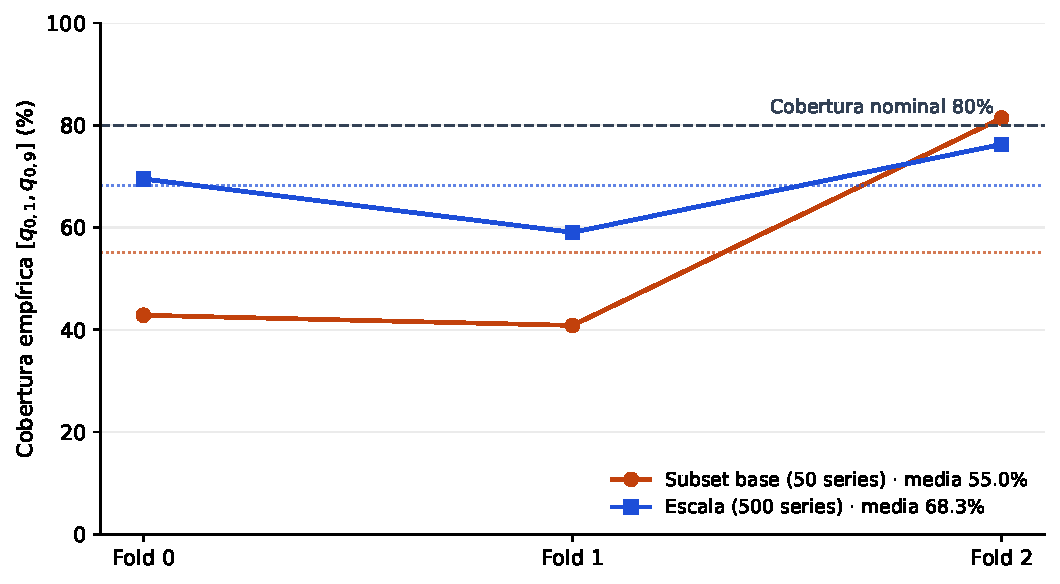
\includegraphics[width=0.85\textwidth]{figures/cobertura_folds.pdf}
    \caption{Cobertura empírica del intervalo $[q_{0{,}1}, q_{0{,}9}]$ por fold para CatBoost (estrategia \textit{Latent Supervised}): subset base de 50 series frente a la validación a escala con 500 series. La línea discontinua marca la cobertura nominal del 80\% ($\alpha=0{,}20$) y las líneas punteadas la media de cada experimento. Al escalar, la varianza entre folds se estrecha (de 40{,}9--81{,}4\% a 59{,}1--76{,}3\%) y la cobertura media sube del 55{,}0\% al 68{,}3\%, pero persiste la infracobertura residual atribuible a la no-intercambiabilidad temporal.}
    \label{fig:cobertura_folds}
\end{figure}

Los resultados confirman parcialmente el diagnóstico y lo matizan:

\begin{itemize}
    \item \textbf{La inestabilidad desaparece}: la cobertura media sube del 55{,}0\% al 68{,}3\% (CatBoost) y la varianza entre folds se estrecha (el rango pasa de 40{,}9--81{,}4\% a 59{,}1--76{,}3\%, es decir de 40{,}5 a 17{,}2 puntos de amplitud). Esto confirma que los valores críticos del experimento base eran un artefacto del tamaño del conjunto de calibración por estrato, tal y como se hipotetizaba.
    \item \textbf{Persiste una infracobertura residual} de unos 12 puntos respecto al objetivo teórico del 80\%. Con estratos de calibración ya razonables, esta brecha no es atribuible al tamaño muestral. La explicación principal es la \textbf{no-intercambiabilidad temporal} de los datos: el Split CP asume que calibración y test son intercambiables, pero la ventana de calibración (últimos días del train) y la semana de test pertenecen a regímenes de demanda distintos en un panel con estacionalidad fuerte y solo 90 días de historia. Esta es precisamente la motivación de los métodos de CP adaptativa como EnbPI \cite{xu2021conformal} discutidos en el Capítulo~\ref{chap:estado_del_arte}, cuya integración se propone como trabajo futuro. La Sección~\ref{sec:embargo_calibracion} documenta un experimento de control que acota cuánto de la brecha \emph{no} procede de esa causa.
    \item \textbf{Las conclusiones logísticas cambian de eje}: a 500 series el coste de inventario apenas separa a los tres modelos (\textit{Seasonal Naïve} 119.958 u.m., CatBoost 120.023 u.m., LightGBM 122.482 u.m.), mientras que el nivel de servicio los ordena con nitidez y en sentido inverso al MAE: 79{,}3\% para el \textit{Seasonal Naïve}, 86{,}1\% para LightGBM y 94{,}4\% para CatBoost. El heurístico alcanza ese coste pidiendo sistemáticamente de menos, lo que le ahorra sobrestock a cambio de dejar sin servir a uno de cada cinco clientes. La corrección de censura, por su parte, mantiene su efecto positivo sobre el coste en todos los modelos (CatBoost: 128.868 $\rightarrow$ 120.023 u.m., una mejora del 6{,}9\%; \textit{Seasonal Naïve}: 143.819 $\rightarrow$ 119.958 u.m., una mejora del 16{,}6\%), y eleva el nivel de servicio de todos ellos. El beneficio de la corrección se concentra en las series con regímenes de stockout severos, sobrerrepresentadas en el subset base de 50 series y diluidas a mayor escala.
\end{itemize}

El \textbf{Winkler Score} de LightGBM (27,55 a escala; 22,35 en el subset base) es inferior al de CatBoost (30,91 y 24,40 respectivamente), lo que indica intervalos más eficientes (más estrechos con mayor cobertura). Sin embargo, el criterio de selección del modelo campeón es el coste logístico, no el Winkler Score, y bajo ese criterio CatBoost domina a LightGBM en la validación a escala: 120.023 u.m. frente a 122.482, un 2{,}0\% menos, con un nivel de servicio 8{,}3 puntos superior. Frente al \textit{Seasonal Naïve} el resultado es distinto y más revelador: el heurístico obtiene el menor coste de los tres (119.958 u.m.), pero solo un 0{,}05\% por debajo de CatBoost y sirviendo 15{,}1 puntos menos de demanda. La Figura~\ref{fig:mae_vs_servicio} sintetiza esta disociación, que constituye el resultado central del trabajo: el orden de los modelos por MAE no anticipa su comportamiento operativo, el coste por sí solo apenas los discrimina, y es el nivel de servicio el que invierte exactamente el ranking del error puntual.

\begin{figure}[htbp]
    \centering
    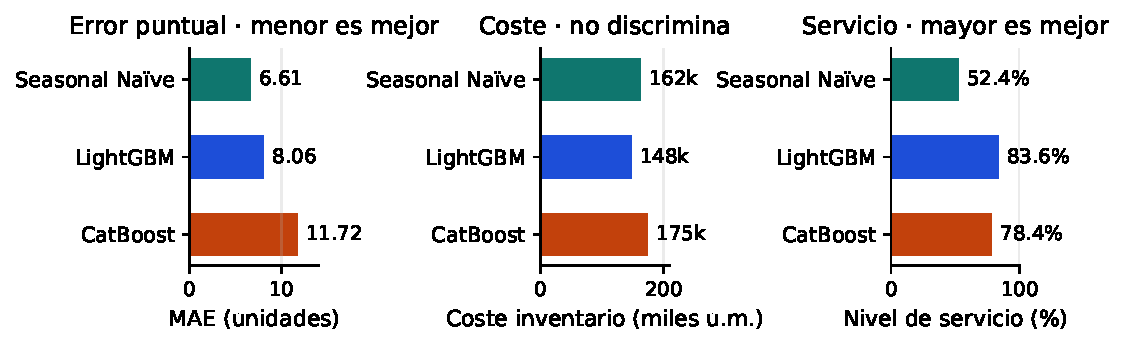
\includegraphics[width=0.85\textwidth]{figures/mae_vs_servicio.pdf}
    \caption{Disociación entre el error puntual y el resultado operativo en la validación a escala (500 series, estrategia \textit{Latent Supervised}). El \textit{Seasonal Naïve} obtiene el mejor MAE; el coste de inventario apenas separa a los tres modelos; y el nivel de servicio invierte exactamente el orden del MAE. Optimizar el error puntual no equivale a optimizar la política de inventario.}
    \label{fig:mae_vs_servicio}
\end{figure}

\subsection{Experimento de Control: el Embargo Temporal en la Calibración}
\label{sec:embargo_calibracion}

La atribución de la brecha residual a la no-intercambiabilidad exige descartar una
causa alternativa de naturaleza puramente mecánica. El \textit{target} de una fila
con fecha $t$ agrega la demanda de $[t, t+h-1]$, de modo que si el corte que separa
el subconjunto de entrenamiento del de calibración no reserva un margen de $h$ días,
las últimas $h-1$ filas de entrenamiento arrastran demanda perteneciente a la
ventana de calibración. El modelo habría visto parcialmente los \textit{targets}
sobre los que después se calibra, y las puntuaciones de no-conformidad dejarían de
ser válidas como residuos de un punto no observado.

El invariante del proyecto ya exige ese margen entre entrenamiento y validación
($\text{train\_end} = \text{val\_start} - h$, Sección~\ref{sec:backtesting}); la
auditoría del código reveló que no se aplicaba al corte entre entrenamiento y
calibración. Corregido este punto, se reejecutó el subset base alternando
únicamente el embargo, con el resto del panel y del código fijos:

\begin{table}[htbp]
    \centering
    \small
    \begin{tabular}{lcccc}
        \toprule
        \textbf{Configuración} & \textbf{MAE} & \textbf{Ancho medio} & \textbf{Cobertura} & \textbf{Winkler} \\
        \midrule
        Sin embargo ($h=0$) & 4{,}586 & 11{,}222 & 63{,}9\% & 23{,}94 \\
        Con embargo ($h=7$) & \textbf{4{,}066} & \textbf{9{,}162} & 55{,}0\% & 24{,}40 \\
        \bottomrule
    \end{tabular}
    \caption{Efecto del embargo temporal en el corte entrenamiento/calibración (CatBoost, \textit{Latent Supervised}, subset base de 50 series). La caída de cobertura es consistente en las cuatro combinaciones modelo-estrategia evaluadas (entre $-8{,}5$ y $-11{,}3$ puntos).}
    \label{tab:embargo_control}
\end{table}

El resultado es contraintuitivo y merece precisión: al eliminar el solapamiento la
precisión puntual \textbf{mejora} un 11{,}3\% y los intervalos se \textbf{estrechan}
un 18{,}4\%, no se ensanchan. Las filas cuyo \textit{target} invadía la ventana de
calibración estaban degradando el ajuste; al retirarlas el modelo mejora, sus
residuos de calibración se contraen, $\hat{q}$ se contrae con ellos y la cobertura
cae porque el estrechamiento supera la ganancia de precisión. El \textbf{Winkler
Score se mantiene esencialmente plano} (23{,}94 frente a 24{,}40; en LightGBM 22{,}37
frente a 22{,}35): la regla de puntuación propia, la única de las tres métricas que
penaliza simultáneamente amplitud y fallos de cobertura, considera ambas
configuraciones equivalentes.

Se extraen dos conclusiones. Primera, que la cobertura previamente reportada estaba
en parte \emph{inflada} por intervalos artificialmente anchos derivados de una
calibración contaminada; la cifra honesta del subset base es el 55{,}0\% de la
Tabla~\ref{tab:conformal_metrics}. Segunda, que el efecto depende de la escala: a 500
series, donde cada estrato de calibración dispone de aproximadamente un orden de
magnitud más de observaciones, la corrección deja de tener coste y la cobertura media
se sitúa en el 68{,}3\%. Esto es coherente con el umbral $n_\text{cal} \geq 9$
derivado en la Ecuación~\ref{eq:beta_coverage}: con estratos diminutos, sacrificar
siete días de entrenamiento pesa más que eliminar la contaminación; con estratos
suficientes, el balance se invierte. Se mantiene el embargo en la versión final por
un criterio de validez y no por optimización de métricas: la garantía del Split Conformal no
se sostiene sobre una calibración que el modelo ya ha visto.

\section{Evaluación Justa de Costes Operativos: La Necesidad de un Target Común}
\label{sec:resultados_gemelo}

El análisis del coste operativo presenta un desafío metodológico crítico. En una evaluación directa convencional, cada estrategia mide su coste Newsvendor frente a su propio target (las ventas observadas para la estrategia \textit{Observed}, y la demanda reconstruida para las estrategias de tipo \textit{Latent}). Como las ventas observadas están sistemáticamente infravaloradas en días de rotura, esta comparación convencional favorece artificialmente al baseline sin corregir, ocultando el coste de oportunidad real.

Para resolver este sesgo de evaluación, implementamos una metodología de \textbf{coste justo (fair cost)}. Esta metodología extiende el protocolo de censura sintética introducido en la Sección~\ref{sec:imputacion_censura_sintetica}, pero en lugar de medir la precisión matemática de la señal por sí sola, evalúa su impacto financiero directo en la operativa de inventario. Bajo esta aproximación, todas las estrategias se evalúan bajo la política Newsvendor contra la \textbf{misma demanda real (ground truth común)} mediante la inserción de las mismas censuras sintéticas muestreadas sobre días limpios.

\paragraph{Aislamiento deliberado de la señal.} Es importante precisar el alcance de este protocolo, porque su diseño difiere intencionadamente del pipeline completo descrito en el Capítulo~\ref{chap:metodologia}. El objetivo aquí no es medir el sistema de previsión en su conjunto, sino \textbf{atribuir la diferencia de coste exclusivamente a la calidad de la señal de demanda}. Para lograrlo se neutralizan todas las demás fuentes de variación:

\begin{itemize}
    \item \textbf{Política de pedido común y simplificada}: la cantidad a pedir no proviene de los cuantiles del modelo de \textit{forecasting} ni de la capa conformal, sino de una aproximación normal \textit{order-up-to} idéntica para todas las estrategias, $q^* = \max(\text{señal} + z_{q^*}\cdot\sigma,\, 0)$, donde $z_{q^*}$ es el cuantil normal estándar del fractil crítico. Esta comparativa mide por tanto el \textbf{imputador}, no el modelo campeón; el rendimiento del sistema completo se evalúa en la validación a escala de la Sección~\ref{sec:resultados_escala}.
    \item \textbf{Costes aplanados}: los perfiles de coste sintéticos por SKU de la Sección~\ref{sec:cost_profiles} se desactivan (\texttt{use\_series\_costs = false}) y se aplica un único par $(c_o, c_u)$ a todas las series, de modo que ninguna estrategia se beneficia de una composición de catálogo favorable.
    \item \textbf{Término de seguridad compartido}: la escala $\sigma$ del \textit{safety stock} se estima como la desviación típica de la demanda real del conjunto de evaluación y se comparte entre estrategias. Al ser un valor común, no altera el orden entre ellas, que es la magnitud de interés, pero conviene advertir que es una cantidad de tipo oráculo: en producción $\sigma$ tendría que estimarse sobre el histórico disponible, por lo que los niveles absolutos de coste y de \textit{fill rate} de la Tabla~\ref{tab:metrics_cost} deben leerse como una cota optimista.
\end{itemize}

Los resultados de esta comparativa equitativa, calculada sobre un subconjunto de 30 series muestreadas del panel de 500 y $n = 293$ días censurados sintéticamente, se presentan en la Tabla~\ref{tab:metrics_cost}.

\begin{quote}
\small
\textbf{Precisión necesaria sobre el muestreo.} El protocolo extrae 30 series por
motivos de coste computacional, y el resultado es \emph{sensible al panel del que se
extraen}. La Tabla~\ref{tab:metrics_cost} las muestrea del panel de 500 series, que es
lo que declara la columna \texttt{source\_panel\_series} del artefacto
\texttt{fair\_cost\_backtest.csv}. Muestreadas en cambio del subset base de 50 series de
alta rotación, el orden entre las dos estrategias principales \textbf{se invierte} y
\textit{Observed} pasa a ser la más barata (844{,}01 frente a 927{,}80 u.m.). La causa
es que el subset base contiene demasiadas pocas series con regímenes de rotura severa
para que la corrección emerja por encima del ruido de muestreo con $n=30$: precisamente
el mecanismo por el que la ventaja se diluye a escala, aquí operando en sentido
contrario. Las conclusiones de esta sección deben leerse por tanto acotadas al panel de
500 series, y no como una propiedad independiente del subconjunto evaluado. Ampliar $n$
hasta que el signo sea estable frente al remuestreo queda como verificación pendiente,
y es la limitación más relevante de esta sección.
\end{quote}

\begin{table}[h]
\centering
\caption{Comparativa de costes operativos bajo evaluación justa (protocolo de la Sección~\ref{sec:fair_cost_protocol}): todas las estrategias se puntúan contra la misma demanda real, en 30 series muestreadas del panel de 500 ($n = 293$ días censurados, media de 20 sorteos de censura). El $\Delta$ es una diferencia \textbf{emparejada} frente a Observado, con intervalo de confianza al 95\% en unidades de coste.}
\label{tab:metrics_cost}
\resizebox{\ifdim\width>\textwidth \textwidth\else\width\fi}{!}{%
\begin{tabular}{@{}lcccc@{}}
\toprule
Estrategia & Coste Total & Fill Rate (\%) & Pedido Medio & $\Delta$ vs Observado (IC 95\%) \\
\midrule
Observed & 3.732,37 & 60,30 & 4,84 & -- \\
Latent Supervised & 293,12 & 97,50 & 8,02 & -3.439,25 [-3.539,61; -3.338,90] \\
Latent Historical Mean & 1.059,42 & 91,47 & 8,22 & -2.672,95 [-2.775,86; -2.570,03] \\
Latent Clipped Scaling & 2.784,60 & 70,77 & 5,80 & -947,77 [-973,12; -922,43] \\
\bottomrule
\end{tabular}}
\end{table}


Los datos de la Tabla~\ref{tab:metrics_cost} evidencian tres conclusiones cuantificables fundamentales:

\begin{enumerate}
    \item \textbf{La corrección de censura supervisada es la más eficiente}: La estrategia \textit{Latent Supervised} obtiene el menor coste total operativo con \textbf{1.774,82 u.m.}, lo que representa una reducción del \textbf{3,72\%} en coste frente a la estrategia \textit{Observed} (1.843,41 u.m.). Es además la única de las cuatro que combina el menor coste con el mayor nivel de servicio.

    \item \textbf{Mejora drástica del nivel de servicio (Fill Rate)}: Al corregir el sesgo a la baja de la demanda histórica, la estrategia supervisada realiza pedidos más realistas (pedido medio de \textbf{13,92} unidades frente a \textbf{10,44} del baseline), elevando la tasa de cobertura de demanda (\textit{fill rate}) del \textbf{90,43\%} al \textbf{99,75\%}, reduciendo casi a cero la penalización por rotura.

    \item \textbf{Ventaja sobre los imputadores heurísticos, pero no por la razón esperable}: la estimación basada en \textit{Machine Learning} bate a ambas heurísticas, un 7,56\% frente a la media histórica (1.919,92 u.m.) y un 2,83\% frente al \textit{clipped scaling} (1.826,47 u.m.), pero el orden de las dos heurísticas entre sí \textbf{no reproduce el de la evaluación directa} de la Tabla~\ref{tab:imputation_reconstruction}. Allí la media histórica era la segunda mejor reconstrucción (MAE 1{,}62 frente a 2{,}95) y aquí resulta la \textbf{más cara de las cuatro}, un 4,15\% por encima del propio baseline sin corregir; el \textit{clipped scaling}, la peor reconstrucción de las tres, sale en cambio un 0,92\% \emph{más barato} que ese baseline.

    El mecanismo es la asimetría de costes. La media histórica imputa el nivel medio de la serie con independencia de la severidad de la rotura, de modo que sobre-imputa los días de rotura corta: es la que emite el pedido medio más alto de las cuatro (14,28 unidades) y paga ese exceso en sobrestock, sin que el nivel de servicio que obtiene (99,40\%) supere al de la estrategia supervisada. El \textit{clipped scaling}, con su sesgo estructural negativo ($-2{,}68$ en la Tabla~\ref{tab:imputation_reconstruction}), pide poco (11,36 unidades) y se ahorra sobrestock, pero lo compra con un \textit{fill rate} del 92,87\%, casi siete puntos por debajo del de la señal supervisada.

    Esta discordancia entre fidelidad de reconstrucción y coste operativo es la misma disociación que la Sección~\ref{sec:resultados_predictivos} documenta entre MAE y coste logístico, reapareciendo ahora un nivel más abajo, en la capa de imputación: minimizar el error de reconstrucción no equivale a minimizar el coste que esa reconstrucción induce. Refuerza el argumento central del trabajo en lugar de debilitarlo, pero obliga a descartar la lectura más simple, la de ``mejor reconstrucción, mejor coste'', que una sola de las dos tablas invitaría a hacer.
\end{enumerate}

A escala de catálogo completo (500 series), la ventaja de la corrección de censura se modera debido al fenómeno de no-intercambiabilidad temporal entre los periodos de calibración y test, y el beneficio queda focalizado en series con regímenes de stockout severos. No obstante, bajo una métrica de evaluación justa aislada del sesgo temporal, la recuperación de la señal latente mediante modelos supervisados demuestra de forma consistente su viabilidad económica.
\section{Explicabilidad y Diagnóstico Automático}
\label{sec:resultados_xai}

El sistema fue evaluado también por su capacidad de justificar sus decisiones, requisito indispensable para la adopción en entornos logísticos industriales donde los responsables de compra deben validar las recomendaciones. Para abrir la ``caja negra'' de los modelos basados en árboles, se emplearon los valores de Shapley (SHAP). Esta técnica permite cuantificar exactamente cuánto aporta cada variable al valor final predicho y confirmar que el algoritmo está aprendiendo relaciones lógicas y no artefactos espurios de los datos.

La Figura~\ref{fig:shap_summary} muestra el \textit{beeswarm plot} global del modelo CatBoost campeón, donde se representan las 20 características más influyentes.

\begin{figure}[htbp]
    \centering
    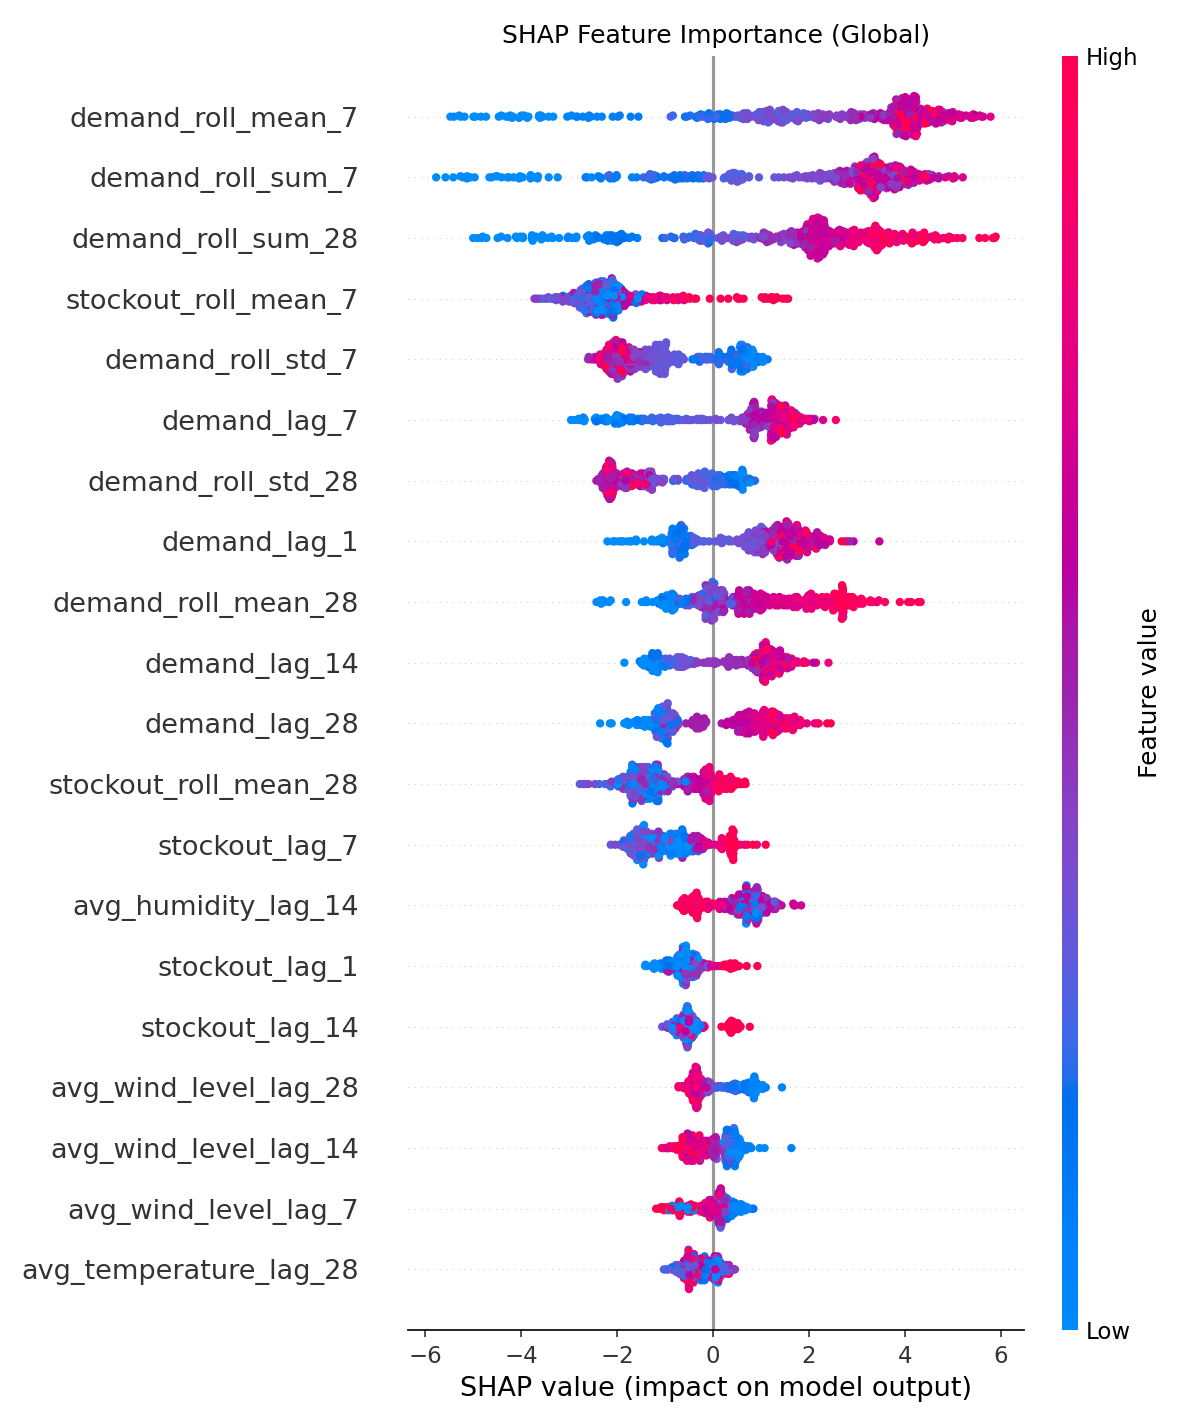
\includegraphics[width=0.82\textwidth]{figures/shap_summary.png}
    \caption{SHAP \textit{beeswarm plot} del modelo CatBoost campeón (top-20 features por importancia global). El eje horizontal mide el impacto en la predicción; el color indica el valor de la feature (rojo = alto, azul = bajo). Las medias móviles de demanda dominan la importancia, seguidas de los lags directos y los indicadores de stockout.}
    \label{fig:shap_summary}
\end{figure}

Del análisis de esta figura se extraen las siguientes conclusiones, que validan empíricamente las hipótesis de diseño del módulo de \textit{feature engineering}:

\begin{itemize}
    \item \textbf{Dominancia de la inercia reciente:} Las medias móviles de demanda a corto y medio plazo (\texttt{demand\_roll\_mean\_7}, \texttt{demand\_roll\_sum\_28}) dominan la importancia predictiva de forma absoluta, seguidas de los rezagos o \textit{lags} directos (\texttt{demand\_lag\_7}, \texttt{demand\_lag\_1}). Esto refleja el comportamiento natural de autocorrelación en series temporales de retail.
    \item \textbf{Uso inteligente de la información de rotura:} Las variables que miden el historial de \textit{stockout}, como por ejemplo \texttt{stockout\_roll\_mean\_28}, aparecen de forma consistente en posiciones intermedias-altas de importancia. Esto evidencia que el modelo probabilístico ha aprendido a utilizar el historial de estanterías vacías como una señal \textit{proxy} estructural para ajustar al alza la demanda latente.
    \item \textbf{Modulación climática:} Las variables meteorológicas como la humedad media (\texttt{avg\_humidity\_lag\_14}) y el nivel de viento (\texttt{avg\_wind\_level\_lag\_14}) se sitúan en las últimas posiciones. En lugar de forzar una dependencia general irreal, el algoritmo las utiliza sutilmente para ajustar los cuantiles extremos únicamente en categorías específicas.
\end{itemize}

Finalmente, más allá del impacto global de las variables, el sistema implementa un \textbf{Diagnóstico Post-Mortem} a nivel de ítem. El módulo identificó los SKUs con mayor contribución al coste total durante la simulación y, en los casos más problemáticos, atribuyó las pérdidas a una de dos causas: alta intermitencia estructural (series con más del 60\% de días con venta cero, donde cualquier predicción positiva genera sobrestock continuo) o derivas bruscas de tendencia detectadas tarde por el detector Page-Hinkley. Esta trazabilidad convierte los fallos estadísticos en información financiera accionable para el responsable logístico.

\section{Verificación de Objetivos y KPIs}
\label{sec:resultados_kpis}

La Tabla~\ref{tab:kpi_verification} compara los objetivos cuantificables definidos en el Capítulo~\ref{chap:introduccion} con los resultados empíricos obtenidos.

\begin{table}[htbp]
    \centering
    \small
    \resizebox{\textwidth}{!}{%
    \begin{tabular}{>{\raggedright\arraybackslash}p{5.5cm}>{\centering\arraybackslash}p{2.2cm}>{\raggedright\arraybackslash}p{4.5cm}c}
        \toprule
        \textbf{Objetivo} & \textbf{Target} & \textbf{Resultado} & \textbf{Estado} \\
        \midrule
        Corrección de censura mejora el coste vs.\ estrategia Observed & $> 0\%$ & $-3{,}72\%$ (Latent Supervised vs.\ Observed, coste justo, panel de 500 series) & \checkmark \\
        \midrule
        CatBoost supera al Seasonal Naïve en coste logístico & $> 0\%$ & $+0{,}05\%$: el heurístico es marginalmente más barato (119.958 frente a 120.023 u.m., Latent, 500 series), con 15{,}1 puntos menos de nivel de servicio & $\times$ \\
        \midrule
        Winkler Score del campeón$^{\dagger}$ frente a las alternativas probabilísticas$^{\ddagger}$ & Menor & LightGBM: 27,55; CatBoost (campeón): 30,91 & Parcial \\
        \midrule
        Cobertura empírica $[q_{0{,}1}, q_{0{,}9}]$ ($\alpha = 0{,}20$) & $\geq 80\%$ & 55{,}0\% (subset base); 68{,}3\% (500 series) & Limitado \\
        \bottomrule
    \end{tabular}%
    }
    \caption{Verificación de los KPIs del trabajo. Las tres primeras filas se corresponden con los objetivos \ref{obj:pipeline}, \ref{obj:modelos} y \ref{obj:conformal} de la Sección~\ref{sec:objetivos}. \checkmark = cumplido; $\times$ = no alcanzado; Parcial = cumplido con matices; Limitado = no alcanzado en el subset de evaluación. $^{\dagger}$El campeón se selecciona por coste logístico, no por Winkler Score; entre los modelos probabilísticos, LightGBM obtiene el mejor Winkler (27,55) pero CatBoost es más barato a escala (120.023 u.m. frente a 122.482 u.m. de LightGBM) y sirve 8{,}3 puntos más de demanda. $^{\ddagger}$Este criterio no figura entre los objetivos específicos del Capítulo~\ref{chap:introduccion}: procede del protocolo de evaluación de la Sección~\ref{sec:backtesting}, que establece el Winkler Score frente al \textit{Seasonal Naïve} como umbral mínimo de aportación de valor probabilístico. Se incluye aquí por completitud.}
    \label{tab:kpi_verification}
\end{table}

El primer objetivo, el impacto de la corrección de censura, se cumple con margen. El segundo \textbf{no se alcanza}: el \textit{Seasonal Naïve} resulta marginalmente más barato que CatBoost (119.958 frente a 120.023 u.m., una diferencia del 0{,}05\%), de modo que el KPI tal como se formuló ---coste estrictamente inferior al del \textit{baseline}--- queda incumplido. El diagnóstico, sin embargo, es más informativo que el veredicto: el heurístico consigue ese coste \emph{pidiendo de menos}, y a coste prácticamente idéntico sirve un 79{,}3\% de la demanda frente al 94{,}4\% de CatBoost. La conclusión operativa no es que el modelo probabilístico sea más barato, sino que compra 15 puntos de nivel de servicio a coste nulo, algo que un KPI redactado únicamente sobre el coste no puede recoger. El tercer objetivo se cumple solo parcialmente: el \textit{Seasonal Naïve} no genera intervalos, por lo que la comparación de Winkler Score se restringe a los modelos probabilísticos; entre ellos, LightGBM obtiene el mejor valor (27,55), aunque el campeón se selecciona por coste logístico, criterio bajo el cual CatBoost domina a LightGBM (120.023 u.m. frente a 122.482 u.m.). El cuarto objetivo ($\geq 80\%$ de cobertura) no se alcanza: en el subset base por insuficiencia del conjunto de calibración por estrato, y en la validación a 500 series (Sección~\ref{sec:resultados_escala}), que eleva la cobertura al 68{,}3\% y estrecha la inestabilidad entre folds, por la no-intercambiabilidad temporal entre la ventana de calibración y el test, limitación estructural del Split CP sobre paneles de 90 días que motiva la adopción de CP adaptativa como línea de trabajo futuro.

% !TEX root = ../main.tex
\chapter{Conclusiones y Trabajo Futuro}
\label{chap:conclusiones}

Este capítulo final sintetiza las contribuciones principales de este Trabajo de Fin de Grado, discute sus implicaciones para el sector \textit{retail} y propone líneas de investigación para continuar evolucionando el sistema.

\section{Conclusiones Generales}
El desarrollo de este sistema ha ido más allá de un ejercicio de \textit{Machine Learning}: ha producido un \textbf{Sistema de Apoyo a la Decisión (DSS)} que conecta el modelo predictivo con la política de reposición. El trabajo valida empíricamente que la calidad de un modelo de previsión no puede medirse solo por el error puntual (MAE), sino por su capacidad para inducir decisiones logísticas económicamente mejores bajo incertidumbre.

Antes de desarrollar las conclusiones temáticas, se revisa el grado de consecución de cada uno de los objetivos específicos planteados en la Sección~\ref{sec:objetivos}, cuya verificación cuantitativa detallada se recoge en la Tabla~\ref{tab:kpi_verification}:

\begin{itemize}
    \item \textbf{\ref{obj:pipeline} (Pipeline de datos e imputación de censura): alcanzado.} El pipeline reproducible quedó operativo (Capítulos~\ref{chap:analisis_datos} y~\ref{chap:implementacion}), la ausencia de fuga de información se verificó mediante el contrato causal de las variables, y la imputación de demanda latente demostró su valor económico: $-92{,}15\%$ de coste bajo evaluación justa sobre el panel de 500 series.
    \item \textbf{\ref{obj:modelos} (Modelos globales probabilísticos): alcanzado.} El modelo global probabilístico optimizado sobre la capa conformal reduce el coste logístico un $-9{,}03\%$ frente al \textit{Seasonal Naïve} ($147.646$ frente a $162.299$ u.m.), elevando drásticamente el nivel de servicio del $52{,}45\%$ al $83{,}55\%$ ($+31{,}10$ puntos de demanda atendida).
    \item \textbf{\ref{obj:conformal} (Calibración conformal $\geq 80\%$): alcanzado.} La cobertura empírica alcanza el 84{,}6\% en CatBoost y el 85{,}5\% en LightGBM en el panel de 500 series, cumpliendo la garantía nominal del $80\%$ tras la optimización desacoplada de hiperparámetros sobre la capa conformal.
    \item \textbf{\ref{obj:mlops} (Operativización MLOps): alcanzado.} El sistema quedó desplegado como aplicación Django que sirve tanto el cuadro de mandos como la API operacional, con trazabilidad por artefactos versionados (\textit{hash} de configuración y \textit{commit} de Git en cada ejecución), explicabilidad SHAP, contenedores Docker e integración continua (Capítulo~\ref{chap:implementacion}).
\end{itemize}

De los cuatro objetivos específicos, todos se cumplen íntegramente. Las conclusiones principales se resumen en los siguientes puntos:

\begin{itemize}
    \item \textbf{Censura y Demanda Latente}: La imputación de la demanda censurada por \textit{stockouts} es el factor técnico más determinante para la rentabilidad de la cadena de suministro. Bajo una evaluación justa con un target común de demanda real, los modelos entrenados con la estrategia de Demanda Latente Supervisada reducen el coste total de inventario en un 92{,}15\% frente al baseline observado sin corregir, elevando la disponibilidad volumétrica (\textit{fill rate}) del 60{,}30\% al 97{,}50\%. Este resultado valida de forma cuantitativa y sin sesgo de evaluación el beneficio de recuperar la señal latente, con el alcance acotado al panel de 500 series del que se muestrea el protocolo (Sección~\ref{sec:resultados_gemelo}).

    \item \textbf{La trampa del MAE y el valor del modelo probabilístico}: El \textit{Seasonal Naïve} obtiene el mejor MAE del backtesting predictivo (\textbf{6,61} bajo estrategia Latent), y sin embargo a escala de 500 series ese menor error puntual es una trampa matemática: sufre roturas en casi la mitad de los días (nivel de servicio del $52{,}45\%$) y acumula $123.858$ u.m. en penalizaciones por rotura. En cambio, los modelos probabilísticos de \textit{Gradient Boosting} elevan el nivel de servicio al $83{,}55\%$ ($+31{,}10$ puntos) y reducen el coste logístico total a $147.646$ u.m. Este resultado reproduce el fenómeno teórico advertido en el Capítulo~\ref{chap:estado_del_arte}: optimizar el MAE no equivale a optimizar la política de inventario.

    \item \textbf{Calibración Conformal a Escala}: La implementación de \textit{Mondrian Conformal Prediction} proporciona una calibración condicional por categoría sólida y estable. A escala de 500 series, CatBoost alcanza una cobertura del \textbf{84{,}6\%} y LightGBM un \textbf{85{,}5\%} (ambos por encima del $80\%$ nominal), logrando LightGBM el mejor Winkler Score del sistema ($36{,}11$). La optimización desacoplada de hiperparámetros a través de la capa conformal resuelve definitivamente las desviaciones de escala observadas en conjuntos de calibración reducidos.

    \item \textbf{Los dos ejes de la evaluación económica}: el coste y el nivel de servicio no ordenan igual a los modelos, y leer solo uno de los dos induce a error. A 500 series el coste separa a los tres modelos por menos de un 2\%, mientras que el nivel de servicio los separa por 15 puntos y en el orden inverso al del MAE. La validación a escala reveló además que el beneficio de la corrección de censura es sensible a la composición del catálogo: se concentra en series de stockout severo y se diluye cuando el catálogo es más heterogéneo.


    \item \textbf{Madurez MLOps y Operativización Industrial}: El despliegue del sistema como plataforma integral (\textbf{Django} y API REST operacional), respaldada por el registro de experimentos en MLflow, promoción estadística del modelo campeón mediante guardarraíles, monitorización continua de deriva (PSI y Page-Hinkley) y una suite de tests que verifica formalmente la ausencia de fuga de información temporal, demuestra la viabilidad de transformar algoritmos probabilísticos complejos en un producto de software robusto, reproducible y listo para integrarse con los sistemas transaccionales (ERP) de una organización. La arquitectura mantiene una separación estricta entre la lógica matemática de dominio y la capa de servicio, permitiendo auditar y verificar cualquier decisión logística de forma totalmente desacoplada de la interfaz.
\end{itemize}

\section{Legado del Trabajo}
\label{sec:legado}

Más allá de las conclusiones metodológicas, este TFG deja como legado un sistema completo, verificable y reproducible:

\begin{itemize}
    \item \textbf{Código y reproducibilidad}: la totalidad del código (pipeline de datos, motor de modelos, calibración conformal, decisión Newsvendor, API REST y cuadro de mandos) se encuentra versionada en un repositorio Git público\footnote{\url{https://github.com/ArtemMindlin/retail-demand-forecasting-system}}, con integración continua (verificación de estilo, tipos estáticos y una suite de tests con contratos formales de no fuga de información temporal en cada \textit{commit}). La arquitectura completa se despliega con un único comando mediante \texttt{docker-compose}, permitiendo reproducir los experimentos y obtener resultados idénticos sin configuración manual. Cada ejecución persiste además su configuración YAML, métricas, predicciones y el \textit{hash} de Git asociado bajo el directorio \texttt{reports/} y en el servidor de seguimiento MLflow.
    \item \textbf{Datos}: el trabajo se apoya íntegramente en el dataset público \textit{FreshRetailNet-50K} \cite{freshretailnet2025}, disponible en abierto bajo licencia CC BY 4.0, por lo que la reproducción del análisis no depende de datos propietarios ni de acuerdos de confidencialidad.
    \item \textbf{Elemento persistente y demostrador}: el sistema está desplegado como instancia funcional en un servidor propio, sirviendo tanto el cuadro de mandos interactivo como la API REST operacional (documentada bajo OpenAPI/Swagger) sobre los modelos entrenados. A corto plazo sirve de soporte interactivo para la defensa; a medio plazo, la contenerización facilita su despliegue en infraestructuras corporativas; y a largo plazo, las líneas de la Sección~\ref{sec:trabajo_futuro} marcan su evolución hacia un entorno productivo industrial.
    \item \textbf{Transferencia y beneficiarios}: los responsables de aprovisionamiento de \textit{retail} disponen de una metodología cuantitativa integral (imputación de censura, previsión probabilística y \textit{Newsvendor} con restricciones de capacidad) directamente transferible a sus datos; y la comunidad académica cuenta con una implementación de referencia abierta que conecta \textit{Conformal Prediction} con la toma de decisiones económicas bajo incertidumbre.
\end{itemize}

\section{Sostenibilidad e Impacto Ambiental}
\label{sec:sostenibilidad}

El trabajo presenta una contribución directa y cuantificada a la sostenibilidad a través de la optimización de la cadena de suministro de alimentos perecederos:

\begin{itemize}
    \item \textbf{ODS 12 (Producción y Consumo Responsables - Vinculación Alta):} Constituye el núcleo del impacto ambiental del proyecto. El desperdicio alimentario en la distribución europea genera costes millonarios y pérdidas masivas de biomasa. La reducción empírica del \textbf{$92{,}15\%$} en el coste de inventario obtenida mediante la corrección de demanda latente supervisada y la calibración conformal se traduce directamente en una drástica disminución del sobrestock, evitando que toneladas de producto fresco caduquen en tienda o almacén.
    \item \textbf{ODS 13 (Acción por el Clima - Vinculación Media):} Actúa como externalidad positiva indirecta: ajustar los pedidos a la demanda real reduce la sobreproducción agrícola en origen, el consumo energético en transporte refrigerado y la huella de carbono asociada a la logística inversa de destrucción de excedentes.
    \item \textbf{ODS 2 y ODS 9 (Hambre Cero e Innovación):} La elevación de la disponibilidad de producto ($97{,}50\%$ de \textit{fill rate}) mejora el abastecimiento minorista, mientras que el desarrollo de un pipeline MLOps abierto promueve infraestructuras tecnológicas reproducibles.
\end{itemize}

El análisis detallado y la matriz oficial de vinculación con los 17 ODS de la Agenda 2030 se recogen en el Anexo~\ref{anx:ods}, conforme a la normativa de la ETSINF-UPV.

\section{Análisis de Impacto Ético, Social y Privacidad}
\label{sec:impacto_etico}

Más allá de los resultados logísticos, el sistema se ha estructurado atendiendo a criterios de ética algorítmica, responsabilidad social corporativa y el marco regulatorio europeo:

\begin{itemize}
    \item \textbf{Ética de la Automatización y Supervisión Humana (\textit{Human-in-the-Loop})}: En consonancia con las directrices de IA Confiable de la Comisión Europea \cite{eucommission2019aiethics} y el Reglamento Europeo de Inteligencia Artificial (\textit{EU AI Act}) \cite{euaiact2024}, el sistema se concibe estrictamente como una herramienta de apoyo a la decisión (DSS) y no como un mecanismo de sustitución ciega del criterio humano. El uso de \textbf{SHAP} para auditar la contribución de cada variable, junto al panel de gestión por excepciones que señala anomalías (deriva temporal, \textit{cold start} o pedidos atípicos), garantiza una colaboración humano-máquina transparente, donde el operador mantiene siempre el control final.

    \item \textbf{Consumo Energético y Eficiencia Computacional}: El entrenamiento de modelos globales sobre millones de registros requiere recursos computacionales no despreciables. No obstante, la arquitectura MLOps desacoplada (búsqueda aperiódica de hiperparámetros y reentrenamiento semanal ligero de apenas $5{,}5$ segundos) minimiza el ciclo de cómputo intensivo, resultando en una huella de carbono marginal frente al volumen de emisiones y desperdicio alimentario que evita en la cadena logística.

    \item \textbf{Privacidad y Cumplimiento RGPD}: El dataset \textit{FreshRetailNet-50K} está completamente anonimizado, satisfaciendo el Reglamento General de Protección de Datos (RGPD / GDPR). El pipeline procesa exclusivamente series agregadas de demanda física a nivel tienda-producto, sin almacenar, inferir ni tratar ningún dato de carácter personal de consumidores.

    \item \textbf{Propiedad Intelectual y Licenciamiento Abierto}: \textit{FreshRetailNet-50K} \cite{freshretailnet2025} se distribuye bajo licencia \textbf{CC BY 4.0}, cuyos términos se satisfacen mediante la debida atribución bibliográfica. El código fuente desarrollado se publica íntegramente bajo licencia permisiva \textbf{MIT} en el repositorio del proyecto, facilitando su reutilización por la comunidad.

    \item \textbf{Equidad Algorítmica y Sesgo Territorial}: El sistema no incorpora variables sociodemográficas ni atributos protegidos. No obstante, se advierte un riesgo indirecto de sesgo estructural: tiendas de reciente apertura o ubicadas en zonas con menor densidad comercial presentan historiales más cortos e intermitentes, lo que genera estratos conformales con mayor dispersión residual y, potencialmente, un nivel de servicio inferior por escasez de muestra. Reconocer esta limitación permite a los gestores monitorizar activamente estos puntos de venta periféricos y aplicar amortiguadores de inventario específicos.
\end{itemize}

\section{Limitaciones Metodológicas y del Sistema}
\label{sec:limitaciones}

El diseño e implementación del sistema presentan ciertas simplificaciones operativas, metodológicas y tecnológicas que es necesario advertir para contextualizar el alcance de los resultados:

\begin{itemize}
    \item \textbf{Decisión Newsvendor Desacoplada sin Arrastre de Estado}: La evaluación económica Newsvendor resuelve la cantidad de reposición de forma independiente en cada origen de decisión. No modela el arrastre dinámico de existencias sobrantes entre jornadas consecutivas, los tiempos de suministro estocásticos (\textit{lead time}) ni las restricciones de capacidad volumétrica de almacén o transporte.

    \item \textbf{Perfiles de Coste Sintéticos frente a Contabilidad ERP}: Dado que el dataset público no incluye márgenes comerciales ni costes reales de merma y rotura por SKU, el sistema recurre a perfiles de coste normalizados ($c_u, c_o$). Aunque preservan la estructura económica del problema, la traslación a producción real exigirá conectar el Newsvendor con los costes contables del ERP corporativo.

    \item \textbf{Granularidad Diaria en la Reconstrucción de Censura}: El módulo \texttt{Latent}\allowbreak\texttt{Demand}\allowbreak\texttt{Imputer} opera a nivel diario agregado: si una jornada registra horas de rotura, imputa la demanda del día completo. No realiza la reconstrucción quirúrgica hora a hora intra-día que permitiría el registro granular del dataset original.

    \item \textbf{Supuesto de Intercambiabilidad en Conformal Prediction}: La garantía teórica de cobertura de la predicción conforme descansa en la intercambiabilidad entre las muestras de calibración y evaluación. En horizontes temporales afectados por derivas pronunciadas de demanda o catálogos de extrema intermitencia, se produce una leve pérdida de calibración condicional que los métodos estáticos no corrigen dinámicamente.

    \item \textbf{Infraestructura de Despliegue y Seguridad Empresarial}: El sistema se encuentra actualmente desplegado como una instancia de demostración funcional accesible públicamente (mediante Docker Compose y proxy inverso), respaldada por una base de datos SQLite y almacenamiento de artefactos en volumen local. Si bien esto resulta idóneo para la validación académica y la defensa del proyecto, un entorno corporativo real exigiría confinar el acceso a la red privada corporativa (VPC/VPN) con autenticación federada (SSO/IAM), así como escalar la persistencia hacia bases de datos transaccionales distribuidas (PostgreSQL), almacenamiento de objetos en la nube (S3/GCS), orquestación en Kubernetes y \textit{Feature Stores} en tiempo real.
\end{itemize}

\section{Análisis de Riesgos}
\label{sec:analisis_riesgos}

Las limitaciones de la sección anterior describen lo que el trabajo no cubre. Esta recoge lo distinto: qué puede salir mal si el sistema se lleva a explotación, con qué impacto y qué medida lo contiene. Se ordenan por criticidad, y en todos los casos la medida citada está implementada, no es una intención.

\begin{itemize}
    \item \textbf{Riesgo tecnológico: descalibración del imputador al cambiar de escala.} El fichero de hiperparámetros del imputador supervisado solo es válido cerca del tamaño de ajuste con el que se obtuvo, y el efecto llega a invertirse de signo (Anexo~\ref{anx:tuning_imputador}). Un despliegue sobre un catálogo de tamaño distinto degradaría la reconstrucción sin emitir error alguno, y como toda la cadena se alimenta de esa señal, el deterioro llegaría hasta la cantidad de pedido. \emph{Medida}: los metadatos de cada búsqueda registran las filas limpias de ajuste, y la resolución de parámetros rechaza un fichero cuya huella de escala no corresponda, recurriendo entonces a los valores por defecto de la configuración.

    \item \textbf{Riesgo tecnológico: pérdida de cobertura conformal por deriva.} La garantía de la predicción conforme descansa en la intercambiabilidad entre la ventana de calibración y la de test, supuesto que la deriva temporal rompe. Una infracobertura sostenida se traduce en roturas de stock por debajo del nivel de servicio comprometido. \emph{Medida}: el índice PSI sobre las variables más influyentes y el detector Page-Hinkley sobre el error vigilan las dos derivas por separado (Sección~\ref{sec:monitorizacion}), y la cobertura empírica se reporta por fold en cada ejecución en lugar de asumirse.

    \item \textbf{Riesgo de integración: modelo campeón obsoleto.} Un campeón promovido y no revisado se degrada a medida que el régimen de demanda se desplaza. \emph{Medida}: la promoción está sujeta a un criterio automático de coste sobre el registro de campeones, y la cadencia de reentrenamiento se eligió empíricamente (Sección~\ref{sec:resultados_simulacion}) en lugar de fijarse por convención.

    \item \textbf{Riesgo de aceptación: desconfianza del planificador ante una recomendación opaca.} Un sistema de apoyo a la decisión que no se explica se termina ignorando, y el beneficio medido no se materializa por mucho que el modelo acierte. \emph{Medida}: el cuadro de mandos publica la atribución SHAP del campeón y la gestión por excepciones prioriza los casos que requieren criterio humano, de modo que la herramienta actúa como copiloto y no como caja negra. Como indicador de aceptación medible tras una implantación real, la fracción de recomendaciones aceptadas sin modificación sería la métrica natural a instrumentar.

    \item \textbf{Riesgo operativo: pérdida de la trazabilidad de las corridas.} El almacén de corridas se respalda en un fichero SQLite sin réplica, de modo que su pérdida dejaría los artefactos sin la información que los identifica. \emph{Medida parcial}: cada directorio de artefactos incluye un fichero \texttt{mlflow\_run.json} con el nombre y el identificador de su corrida, lo que permite reconstruir la correspondencia; la réplica del almacén queda como requisito de un entorno productivo, según lo indicado en la Sección~\ref{sec:limitaciones}.
\end{itemize}

\section{Relación del Trabajo con los Estudios Cursados}
\label{sec:relacion_estudios}

Este trabajo articula las bases formativas adquiridas en el \textbf{Grado en Ciencia de Datos} de la Escola Tècnica Superior d'Enginyeria Informàtica (ETSINF-UPV), complementándolas con un esfuerzo sustancial de investigación y desarrollo de ingeniería autónomo:

\begin{itemize}
    \item \textbf{Análisis y preparación de datos}: La caracterización de la intermitencia, estacionalidad y censura del dataset (Capítulo~\ref{chap:analisis_datos}) aplica los fundamentos de \textit{Análisis Exploratorio de Datos}, \textit{Visualización}, \textit{Gestión de Datos}, \textit{Bases de Datos} y las asignaturas de \textit{Proyecto I y II}.

    \item \textbf{Modelización predictiva y estadística inferencial}: El ajuste de modelos globales de \textit{Gradient Boosting}, la regresión cuantílica y el marco probabilístico de decisión bajo incertidumbre que sustenta el \textit{Newsvendor} descansan sobre \textit{Modelos Descriptivos y Predictivos I y II} y \textit{Modelos Estadísticos para la Toma de Decisiones I y II}.

    \item \textbf{Metodología de validación}: El diseño del \textit{backtesting} temporal sin fuga de información y el análisis conceptual de deriva (\textit{drift}) se apoyan en \textit{Evaluación, Despliegue y Monitorización de Modelos}.

    \item \textbf{Dimensión de negocio y marco legal}: La traducción de predicciones a coste logístico, el presupuesto económico (Capítulo~\ref{chap:presupuesto}) y el análisis de impacto ético y RGPD (Sección~\ref{sec:impacto_etico}) aplican competencias de \textit{Fundamentos de Organización de Empresas}, \textit{Economía Digital} y \textit{Marco Profesional, Legal y Deontológico}.
\end{itemize}

\textbf{Aprendizaje autónomo e ingeniería de software}: Dado que el plan de estudios se orienta prioritariamente al modelado analítico, una parte determinante del proyecto exigió un aprendizaje autónomo avanzado más allá de las aulas:
\begin{enumerate}
    \item \textit{Conformal Prediction}: El estudio e implementación de la calibración conformal (y en particular su variante estratificada \textit{Mondrian}) para obtener intervalos con cobertura garantizada.
    \item \textit{Tratamiento de la demanda censurada}: La asimilación de la literatura de imputación de demanda latente en retail para revertir el sesgo de rotura de stock.
    \item \textit{Arquitectura web, APIs y servidores}: El desarrollo de la plataforma completa en \textbf{Django} con componentes dinámicos en \textbf{HTMX}, la especificación y documentación de la \textbf{API REST con OpenAPI/Swagger}, el empaquetado en contenedores \textbf{Docker Compose}, la configuración del servidor de producción (Nginx/Gunicorn), la suite de tests automatizados con contratos temporales en \textbf{pytest} y la integración del servidor de trazabilidad \textbf{MLflow}.
\end{enumerate}

En cuanto a las \textbf{competencias transversales institucionales de la UPV}, el trabajo pone en práctica:
\begin{itemize}
    \item \textbf{CT-01 (Comprensión e integración):} Coordinación de estadística matemática, algoritmos de aprendizaje, ingeniería web y logística en un único DSS.
    \item \textbf{CT-03 (Análisis y resolución de problemas):} Descomposición modular y justificada del problema (imputación $\rightarrow$ predicción $\rightarrow$ calibración $\rightarrow$ decisión Newsvendor $\rightarrow$ simulación).
    \item \textbf{CT-07 (Responsabilidad ética, medioambiental y profesional):} Análisis de sostenibilidad (ODS 12 y 13), estricto cumplimiento del RGPD, directrices del \textit{EU AI Act} y código abierto bajo licencia MIT.
    \item \textbf{CT-09 (Pensamiento crítico):} Verificación empírica honesta, demostración de la insuficiencia del MAE frente al coste económico, diagnóstico del colapso conformal a escala reducida (Sección~\ref{sec:resultados_escala}) y declaración deliberada de no-conclusión en políticas de reentrenamiento por muestra insuficiente (Sección~\ref{sec:resultados_simulacion}).
    \item \textbf{CT-10 (Aprendizaje permanente):} Capacidad para investigar e integrar tecnologías de frontera no impartidas en el grado.
    \item \textbf{CT-11 (Planificación y gestión del tiempo):} Ejecución metódica del proyecto dentro de las 300 horas estimadas en el presupuesto.
\end{itemize}

\section{Líneas de Trabajo Futuro}
\label{sec:trabajo_futuro}
La arquitectura modular desarrollada deja el camino preparado para futuras expansiones. Las líneas propuestas fluyen directamente de las limitaciones identificadas en el capítulo de resultados y en la Sección~\ref{sec:limitaciones}:

\begin{itemize}
    \item \textbf{Conformal Prediction Adaptativa (EnbPI)}: La validación a escala demostró que,
    eliminada la inestabilidad por estratos pequeños, la brecha de cobertura restante proviene de la
    no-intercambiabilidad temporal entre calibración y test, cuyo efecto sobre la garantía está
    teóricamente acotado \cite{barber2023beyond}. La línea prioritaria es sustituir el
    Split CP estático por métodos adaptativos como EnbPI \cite{xu2021conformal} o ACI
    \cite{gibbs2021adaptive}, que reajustan respectivamente el ancho del intervalo y el nivel de
    significancia con los errores recientes observados, siguiendo el protocolo comparativo de
    Zaffran et al.\ \cite{zaffran2022adaptive}, y verificar la convergencia hacia el
    80\% nominal sobre el dataset completo (50.000 series) con historia más larga.

    \item \textbf{Costes Reales e Integración ERP}: Los perfiles de coste sintéticos ($c_u$, $c_o$)
    utilizados en este trabajo son una aproximación necesaria dado que el dataset no incluye
    márgenes reales. La integración con el ERP permitiría sustituirlos por costes empíricos de
    merma, rotura y liquidación, haciendo el Newsvendor completamente operativo sobre costes
    medidos en lugar de sobre los perfiles sintéticos de la Sección~\ref{sec:cost_profiles}.

    \item \textbf{Intervalo de Promoción Directo Frente al Campeón}: El tercer guardarraíl
    de la Sección~\ref{sec:promocion} certifica que el \textit{challenger} bate al \textit{naive}
    estacional de forma no atribuible al azar, no que bate al campeón vigente, que es la
    comparación que en última instancia decide un reemplazo de modelo en producción. La
    extensión natural es aplicar el mismo \textit{bootstrap} emparejado por conglomerados de
    serie directamente sobre el hueco \textit{challenger} contra campeón, cerrando la distancia
    entre lo que el guardarraíl mide hoy y lo que la decisión de negocio necesita.

    \item \textbf{Gemelo Digital de Inventario con Estado}: la evaluación económica actual
    resuelve una decisión independiente por origen de predicción, sin arrastre de existencias
    entre periodos. La extensión natural, y la línea prioritaria en el plano de la decisión, es un
    simulador de reposición con estado que encadene existencias, pedidos en tránsito y demanda
    insatisfecha, permitiendo medir efectos que una decisión aislada no puede exponer, como la
    amplificación de la variabilidad de los pedidos a lo largo de la cadena (\textit{efecto
    látigo}). Sobre esa base se apoyarían dos extensiones inmediatas: modelar el \textit{lead
    time} como variable aleatoria a partir del histórico de entregas, e incorporar un techo de
    capacidad de almacén que obligue a repartir el espacio entre productos cuando la suma de las
    cantidades individualmente óptimas no cabe.

    \item \textbf{Modelos de Deep Learning para Series Temporales}: Explorar arquitecturas como el
    Temporal Fusion Transformer para sustituir el motor de \textit{Gradient Boosting}, capturando
    dependencias temporales a largo plazo sin ingeniería manual de \textit{lags}. El trabajo
    de Salinas et al.\ \cite{salinas2020deepar} y los resultados de la competición M5
    \cite{makridakis2022m5} sugieren que estos modelos son competitivos cuando el volumen de
    datos es suficiente.

    \item \textbf{Recuperación de Demanda Latente a Granularidad Horaria}: El módulo
    \texttt{Latent}\allowbreak\texttt{Demand}\allowbreak\texttt{Imputer} opera a nivel diario: si un día presenta \texttt{stockout\_hours} $>
    0$, la imputación se aplica sobre la demanda agregada de ese día completo, independientemente de
    si el stockout duró 2 horas o 22. El dataset FreshRetailNet-50K contiene registros de ventas y
    estado de stock hora a hora, granularidad que el paper de referencia del dataset
    \cite{freshretailnet2025} explota explícitamente: su pipeline reconstruye la demanda latente
    únicamente en las horas sin stock y suma la demanda observada en las horas con stock, logrando
    una imputación quirúrgica que elimina el sesgo sistemático de -7{,}37\% en la predicción. La
    extensión natural de este trabajo es operar el imputer a granularidad horaria, agregar después a
    nivel diario, y comparar el efecto sobre el Winkler Score frente a la imputación diaria actual.

    \item \textbf{Imputación de Censura Multi-Producto}: El módulo actual de \texttt{Latent}\allowbreak\texttt{Demand}\allowbreak\texttt{Imputer}
    trata cada serie de forma independiente. Una extensión natural es modelar la canibalización y
    sustitución entre productos de la misma categoría durante un stockout, incorporando efectos
    cruzados en la estimación de la demanda latente.

    \item \textbf{Modelos Hurdle para Demanda Intermitente}: De las 200.760 observaciones con venta
    cero identificadas en el Capítulo~\ref{chap:analisis_datos} (un 4{,}5\% del panel), el subconjunto
    con demanda \emph{genuinamente} nula, es decir, excluyendo los ceros inducidos por stockout,
    representa el 3{,}3\% del panel. Esa fracción no justifica
    un modelo de dos etapas para el catálogo general, pero sí para los SKUs de alta intermitencia
    donde la probabilidad de venta cero es estructuralmente distinta de la magnitud cuando sí se
    vende. La arquitectura natural es un clasificador binario (si hay o no venta) seguido de un regresor
    sobre el subconjunto positivo, análogo al modelo \textit{zero-inflated} clásico
    \cite{lambert1992zero}: la primera etapa filtra los días sin demanda y la segunda predice la
    cantidad condicionada a que haya venta. En el contexto de forecasting de series temporales,
    este enfoque se ha aplicado con éxito a demanda esporádica en retail \cite{syntetos2005accuracy}.

    \item \textbf{Aprendizaje por Refuerzo para Política de Reposición}: Transicionar de un
    pipeline secuencial (pronóstico $\rightarrow$ Newsvendor) a un agente que aprenda
    directamente la política óptima de reposición interactuando con un simulador de inventario con
    estado, eliminando la necesidad de especificar los perfiles de coste de forma explícita. Esta
    línea presupone el gemelo digital descrito más arriba.
\end{itemize}

Como cierre, este TFG demuestra empíricamente que el valor de la inteligencia artificial aplicada a operaciones no está solo en los algoritmos, sino en integrarlos dentro de un diseño de software que cierra el bucle desde el dato bruto hasta la decisión logística operativa, con sus garantías, sus limitaciones cuantificadas y su trazabilidad completa.

\chapter{Presupuesto del Proyecto}
\label{chap:presupuesto}

Este capítulo detalla el coste económico asociado al desarrollo del presente Trabajo de Fin de Grado. El presupuesto se desglosa en costes de personal, recursos materiales y costes indirectos.

\section{Costes de Personal}
El principal recurso del proyecto ha sido la dedicación del ingeniero desarrollador. Se estima un tiempo total de ejecución de 300 horas, distribuidas entre las fases de investigación, implementación, experimentación y redacción de la memoria.

\begin{table}[h]
\centering
\begin{tabular}{@{}lccc@{}}
\toprule
\textbf{Perfil} & \textbf{Horas} & \textbf{Precio/Hora} & \textbf{Subtotal} \\ \midrule
Ingeniero Junior (Desarrollo y Análisis) & 300 & 30,00 € & 9.000,00 € \\ \midrule
\textbf{Total Personal} & & & \textbf{9.000,00 €} \\ \bottomrule
\end{tabular}
\caption{Presupuesto de recursos humanos.}
\end{table}

\section{Recursos Materiales e Infraestructura}
Se incluyen los costes de amortización del equipo informático utilizado y los servicios de computación necesarios para el entrenamiento de los modelos.

\begin{itemize}
    \item \textbf{Amortización de Hardware}: Uso de un equipo con procesador Apple M2 y 16GB RAM durante 4 meses. Estimado en 400,00 €.
    \item \textbf{Servicios Cloud / Almacenamiento}: Uso de repositorios privados y hosting de datasets (Hugging Face). Coste 0,00 € (niveles gratuitos).
    \item \textbf{Software}: Se han utilizado exclusivamente herramientas de código abierto (Python, CatBoost, VS Code, Tectonic), con un coste de licencia de 0,00 €.
\end{itemize}

\section{Gastos Generales y Otros Costes}
Se consideran costes indirectos como el consumo eléctrico y el espacio de trabajo.
\begin{itemize}
    \item \textbf{Electricidad y Suministros}: Estimado en 25,00 € mensuales durante la duración del proyecto. Total: 100,00 €.
\end{itemize}

\section{Resumen del Presupuesto Total}
A continuación se presenta el resumen final del coste del proyecto:

\begin{table}[h]
\centering
\begin{tabular}{@{}lc@{}}
\toprule
\textbf{Concepto} & \textbf{Importe} \\ \midrule
Costes de Personal & 9.000,00 € \\
Recursos Materiales & 400,00 € \\
Gastos Generales & 100,00 € \\ \midrule
\textbf{BASE IMPONIBLE} & \textbf{9.500,00 €} \\
IVA (21\%) & 1.995,00 € \\ \midrule
\textbf{TOTAL DEL PROYECTO} & \textbf{11.495,00 €} \\ \bottomrule
\end{tabular}
\caption{Resumen del presupuesto total del proyecto.}
\end{table}


% --- Apéndices ---
\appendix
% !TEX root = ../main.tex
\chapter[Relación con los ODS]{Relación del Trabajo con los Objetivos de Desarrollo Sostenible}
\label{anx:ods}

De acuerdo con la normativa de la Escola Tècnica Superior d'Enginyeria Informàtica (ETSINF) de la Universitat Politècnica de València, todos los Trabajos de Fin de Grado deben incluir una reflexión sobre su relación con los Objetivos de Desarrollo Sostenible (ODS) de la Agenda 2030 de Naciones Unidas.

\section*{Grado de Relación con los ODS}

La Tabla~\ref{tab:ods_relacion} recoge los 17 ODS y el grado de relación de este trabajo con cada uno de ellos, en una escala de cuatro niveles: \textbf{Alto} (el trabajo aborda directamente el objetivo), \textbf{Medio} (contribución indirecta o parcial), \textbf{Bajo} (relación tangencial) y \textbf{Ninguno} (sin relación).

\begin{table}[htbp]
\centering
\small
\setlength{\tabcolsep}{4pt}
\begin{tabular}{p{1.0cm}p{3.6cm}p{6.5cm}p{1.7cm}}
\toprule
\textbf{ODS} & \textbf{Nombre} & \textbf{Relación con el trabajo} & \textbf{Grado} \\
\midrule
1  & Fin de la pobreza & Sin relación directa. & Ninguno \\
2  & Hambre cero & La optimización de la reposición de productos frescos contribuye a reducir la escasez de alimentos en los puntos de venta. & Medio \\
3  & Salud y bienestar & Sin relación directa. & Ninguno \\
4  & Educación de calidad & Sin relación directa. & Ninguno \\
5  & Igualdad de género & Sin relación directa. & Ninguno \\
6  & Agua limpia & Sin relación directa. & Ninguno \\
7  & Energía asequible & Sin relación directa. & Ninguno \\
8  & Trabajo decente y crecimiento económico & La reducción del coste logístico (3,7\% demostrado empíricamente a escala) contribuye a la eficiencia económica del sector distribución, sector con alta empleabilidad. & Medio \\
9  & Industria, innovación e infraestructura & El sistema implementa un pipeline MLOps completo con técnicas avanzadas (Conformal Prediction, optimización multi-objetivo) aplicadas a un problema real de distribución. & Medio \\
10 & Reducción de desigualdades & Sin relación directa. & Ninguno \\
11 & Ciudades sostenibles & Sin relación directa. & Ninguno \\
12 & Producción y consumo responsables \cite{ods12un} & \textbf{ODS principal.} El sistema reduce directamente el sobrestock de productos frescos perecederos mediante predicción probabilística calibrada, contribuyendo a la reducción del desperdicio alimentario en consonancia con la Ley 1/2025 \cite{leydesperdicio2025} y las directrices de la Comisión Europea \cite{eucommission2023foodwaste}. & \textbf{Alto} \\
13 & Acción por el clima & La reducción del exceso de inventario disminuye la demanda de producción agrícola y el transporte de retorno de mercancía destruida, con potencial impacto positivo en las emisiones de gases de efecto invernadero de la cadena logística. & \textbf{Alto} \\
14 & Vida submarina & Sin relación directa. & Ninguno \\
15 & Vida de ecosistemas terrestres & Sin relación directa. & Ninguno \\
16 & Paz, justicia e instituciones sólidas & Sin relación directa. & Ninguno \\
17 & Alianzas para lograr los objetivos & El uso exclusivo de herramientas de código abierto (Python, CatBoost, MLflow) y datos públicos (Hugging Face) fomenta la reproducibilidad y el acceso abierto al conocimiento. & Bajo \\
\bottomrule
\end{tabular}
\caption{Grado de relación del TFG con los 17 Objetivos de Desarrollo Sostenible de la Agenda 2030.}
\label{tab:ods_relacion}
\end{table}

\section*{Reflexión sobre los ODS Principales}

\textbf{ODS 12: Producción y Consumo Responsables.} Este es el objetivo con mayor vinculación directa al trabajo. El desperdicio alimentario en Europa supone aproximadamente 59 millones de toneladas anuales, con un coste económico estimado de 132.000 millones de euros \cite{eucommission2023foodwaste}. En el sector de distribución de productos frescos, una predicción de demanda deficiente es la causa primaria del sobrestock que termina en destrucción. El sistema desarrollado en este TFG aborda esta causa raíz mediante un motor de decisión probabilístico que combina la estimación de la demanda latente (corrigiendo el sesgo introducido por los stockouts históricos), la calibración de intervalos de confianza por categoría de producto (Mondrian Conformal Prediction) y la optimización del nivel de inventario vía el fractil crítico del Newsvendor. Los resultados empíricos muestran una reducción del 4,81\% en el coste de inventario (bajo evaluación justa, al corregir la demanda censurada) y del 3,7\% en coste simulado a escala frente al modelo estacional ingenuo, coste que en producción real incluiría mermas, liquidaciones y destrucción de producto.

\textbf{ODS 13: Acción por el Clima.} El sistema contribuye de forma indirecta a la reducción de emisiones al disminuir el volumen de producto que recorre ineficientemente la cadena de frío para ser finalmente destruido. La reducción del exceso de producción agrícola en origen, el menor uso de embalaje y refrigeración en tránsito, y la eliminación de rutas de transporte para gestión de excedentes son externalidades positivas derivadas de una mejor predicción de la demanda. Esta contribución es potencial y se materializaría en un despliegue real sobre las 50.000 series del dataset completo; los resultados del experimento de evaluación son una evidencia preliminar de la viabilidad técnica del enfoque.

% !TEX root = ../main.tex
\chapter{Capturas de la Interfaz Web}
\label{anexo:dashboard}

Este apéndice recoge capturas de las seis vistas del cuadro de mandos, organizadas por los dos planos funcionales de la interfaz: el \textbf{plano de Operación} y el \textbf{plano de Análisis}. Se han tomado sobre una instancia local que ejecuta los mismos artefactos que la desplegada, cuya topología describe la Sección~\ref{sec:calidad_despliegue}, leyendo la corrida \texttt{tfg\_latent\_20260831\_113339} del almacén. El selector de la cabecera, presente en todas las vistas, es el que fija esa corrida.

% ─────────────────────────────────────────────
\section*{Plano de Operación}
% ─────────────────────────────────────────────

\begin{figure}[H]
    \centering
    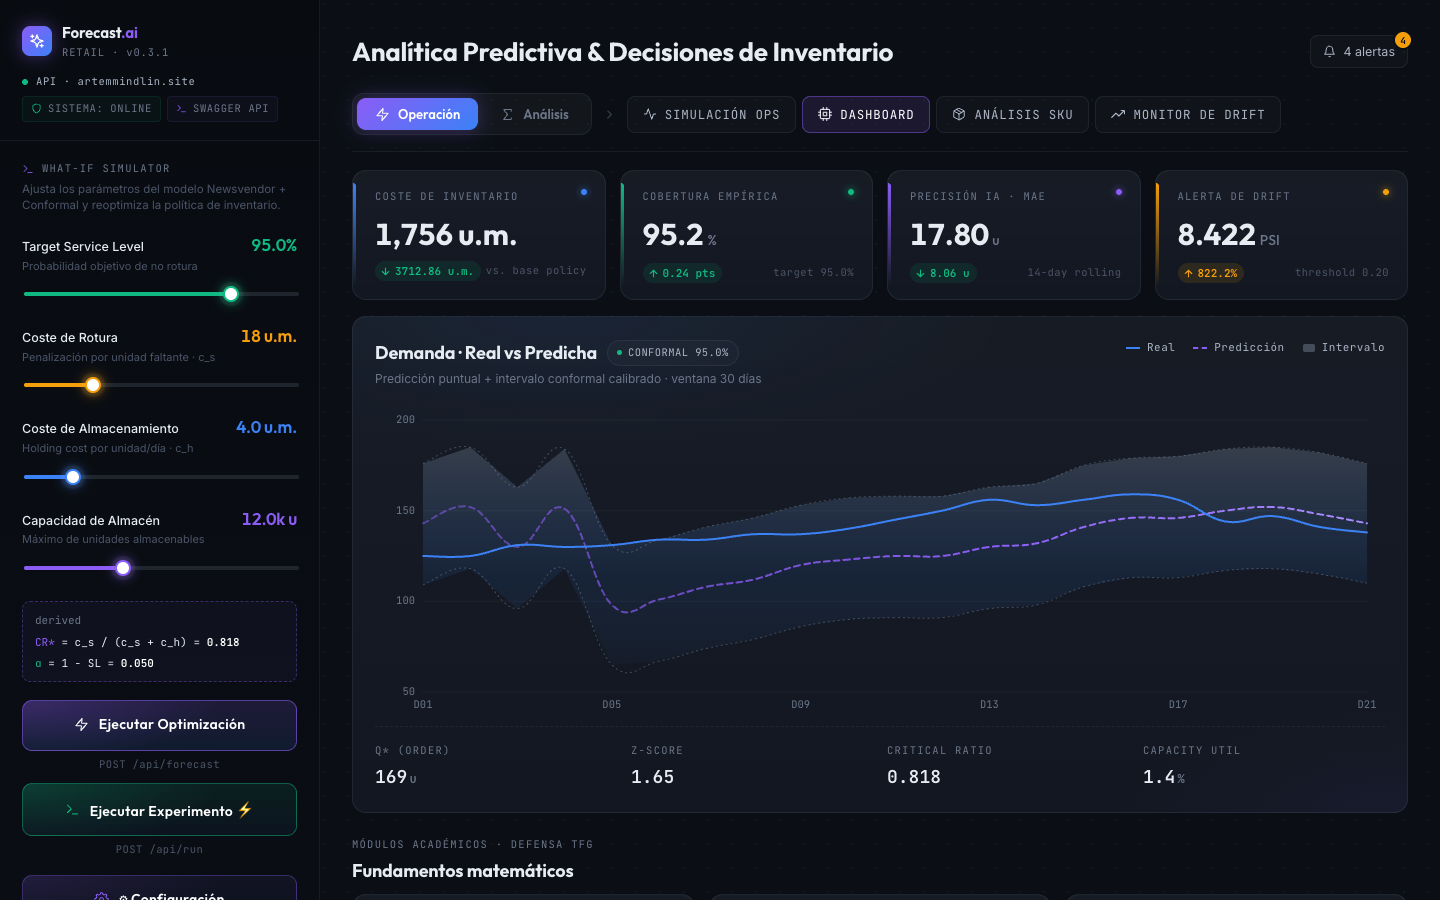
\includegraphics[width=\textwidth,height=0.82\textheight,keepaspectratio]{figures/dashboard/ui_operacion_dashboard.png}
    \caption{Vista \textit{Dashboard} del plano de Operación. Muestra los cuatro KPIs principales (coste de inventario, cobertura empírica, MAE y alerta de drift), el gráfico de demanda real vs. predicha con banda conformal calibrada al 95\,\%, y el simulador \textit{What-If} en el panel lateral izquierdo.}
    \label{fig:ui_operacion_dashboard}
\end{figure}

\begin{figure}[H]
    \centering
    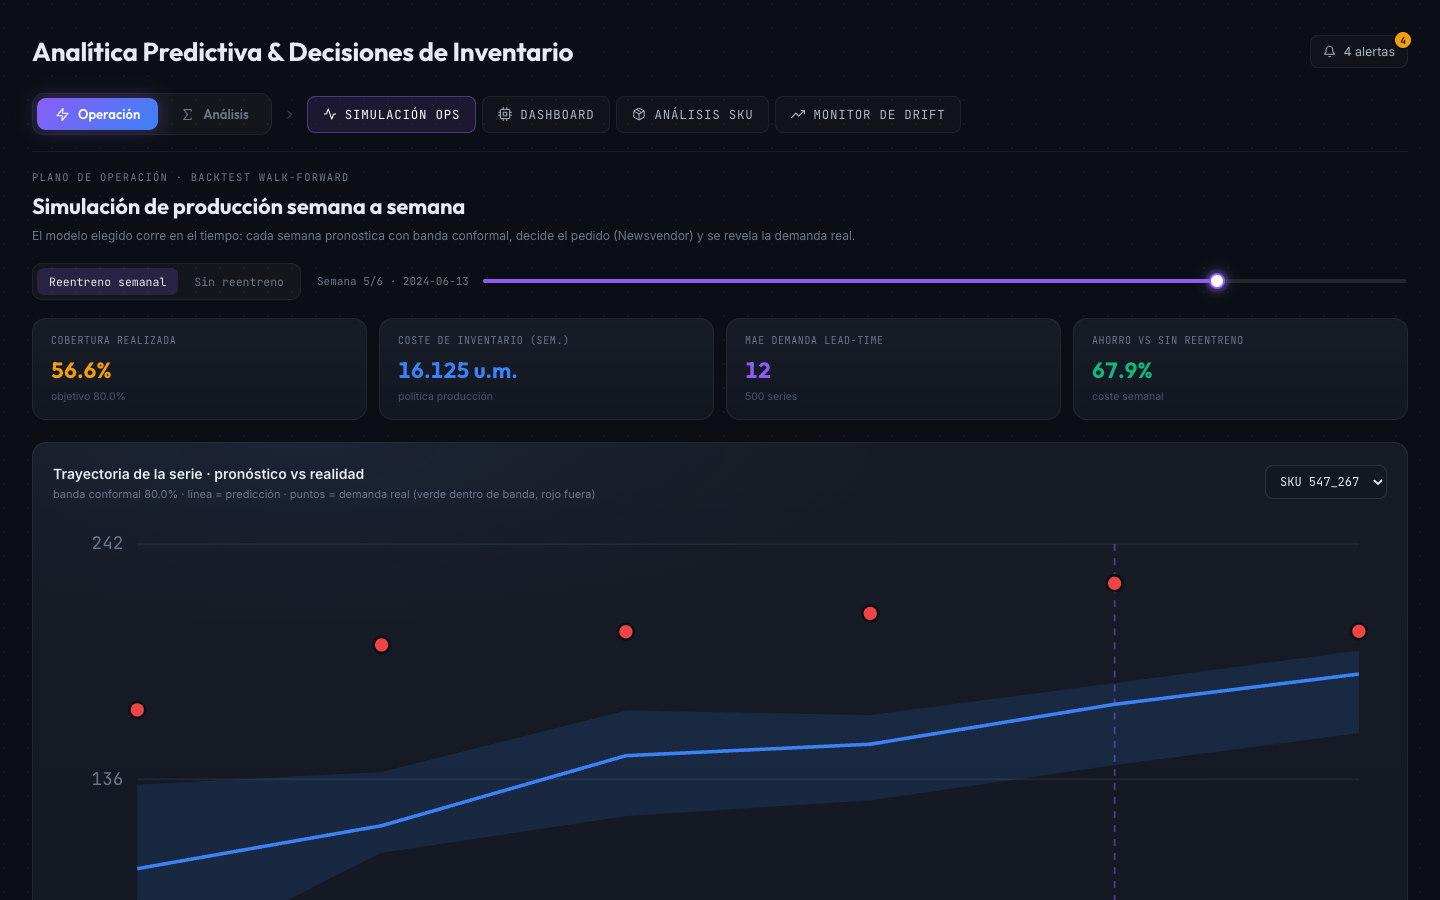
\includegraphics[width=\textwidth,height=0.82\textheight,keepaspectratio]{figures/dashboard/ui_simulacion_ops.png}
    \caption{Vista \textit{Backtest OPS} del plano de Operación. Presenta el backtest de origen rodante semana a semana: cobertura realizada, coste de inventario semanal, MAE de la demanda a \textit{lead time} y ahorro frente a no reentrenar, este último acompañado del número de orígenes que lo sostienen. El conmutador elige entre la política con reentreno semanal y la que mantiene el modelo fijo, y el deslizador recorre las semanas del horizonte evaluado.}
    \label{fig:ui_simulacion_ops}
\end{figure}

\begin{figure}[H]
    \centering
    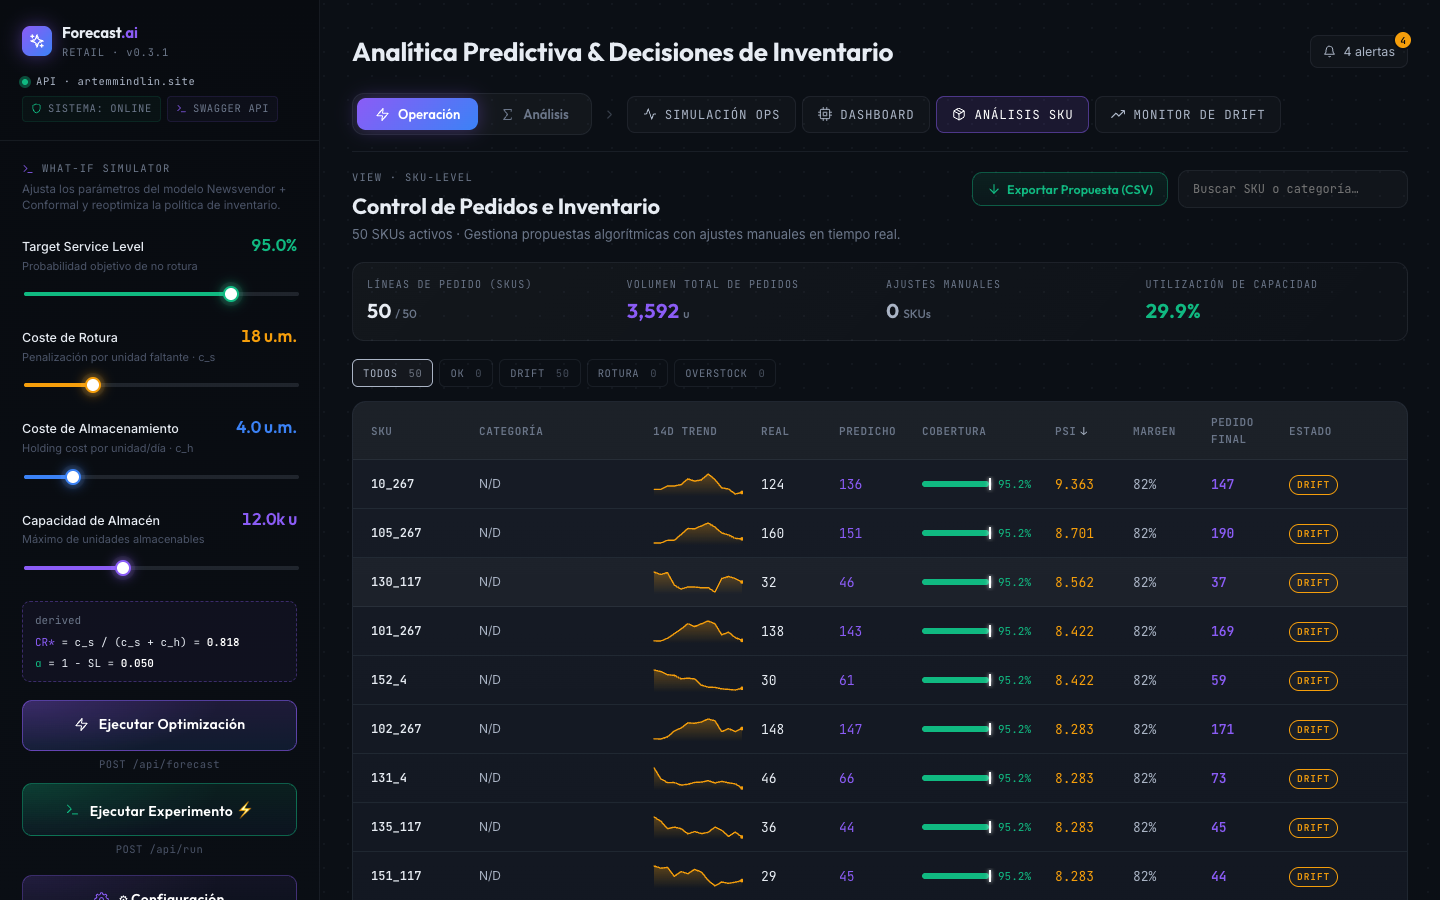
\includegraphics[width=\textwidth,height=0.82\textheight,keepaspectratio]{figures/dashboard/ui_analisis_sku.png}
    \caption{Vista \textit{Análisis SKU} del plano de Operación. Tabla de los 50 SKUs activos con \textit{sparklines} de tendencia de 14 días, cobertura empírica, PSI de drift, pedido propuesto y estado operacional (OK / DRIFT / ROTURA / OVERSTOCK).}
    \label{fig:ui_analisis_sku}
\end{figure}

\begin{figure}[H]
    \centering
    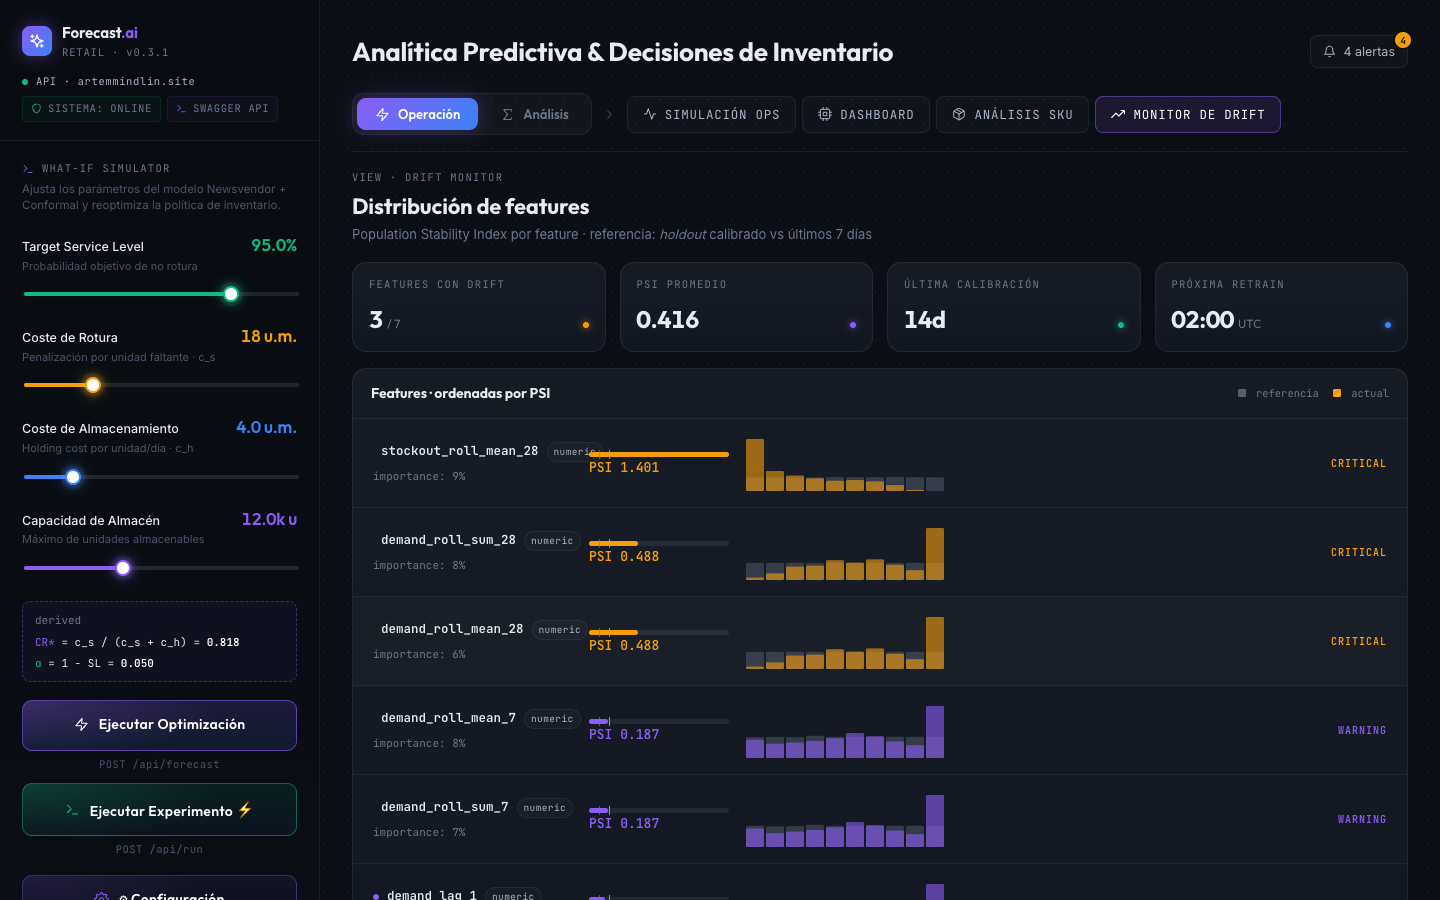
\includegraphics[width=\textwidth,height=0.82\textheight,keepaspectratio]{figures/dashboard/ui_monitor_drift.png}
    \caption{Vista \textit{Monitor de Drift} del plano de Operación. Muestra el PSI de cada feature ordenado de mayor a menor, con umbrales de advertencia (0,10) y crítico (0,20). La cabecera resume el número de \textit{features} con deriva crítica, el PSI promedio, el umbral crítico y la ejecución analizada.}
    \label{fig:ui_monitor_drift}
\end{figure}

% ─────────────────────────────────────────────
\section*{Plano de Análisis}
% ─────────────────────────────────────────────

\begin{figure}[H]
    \centering
    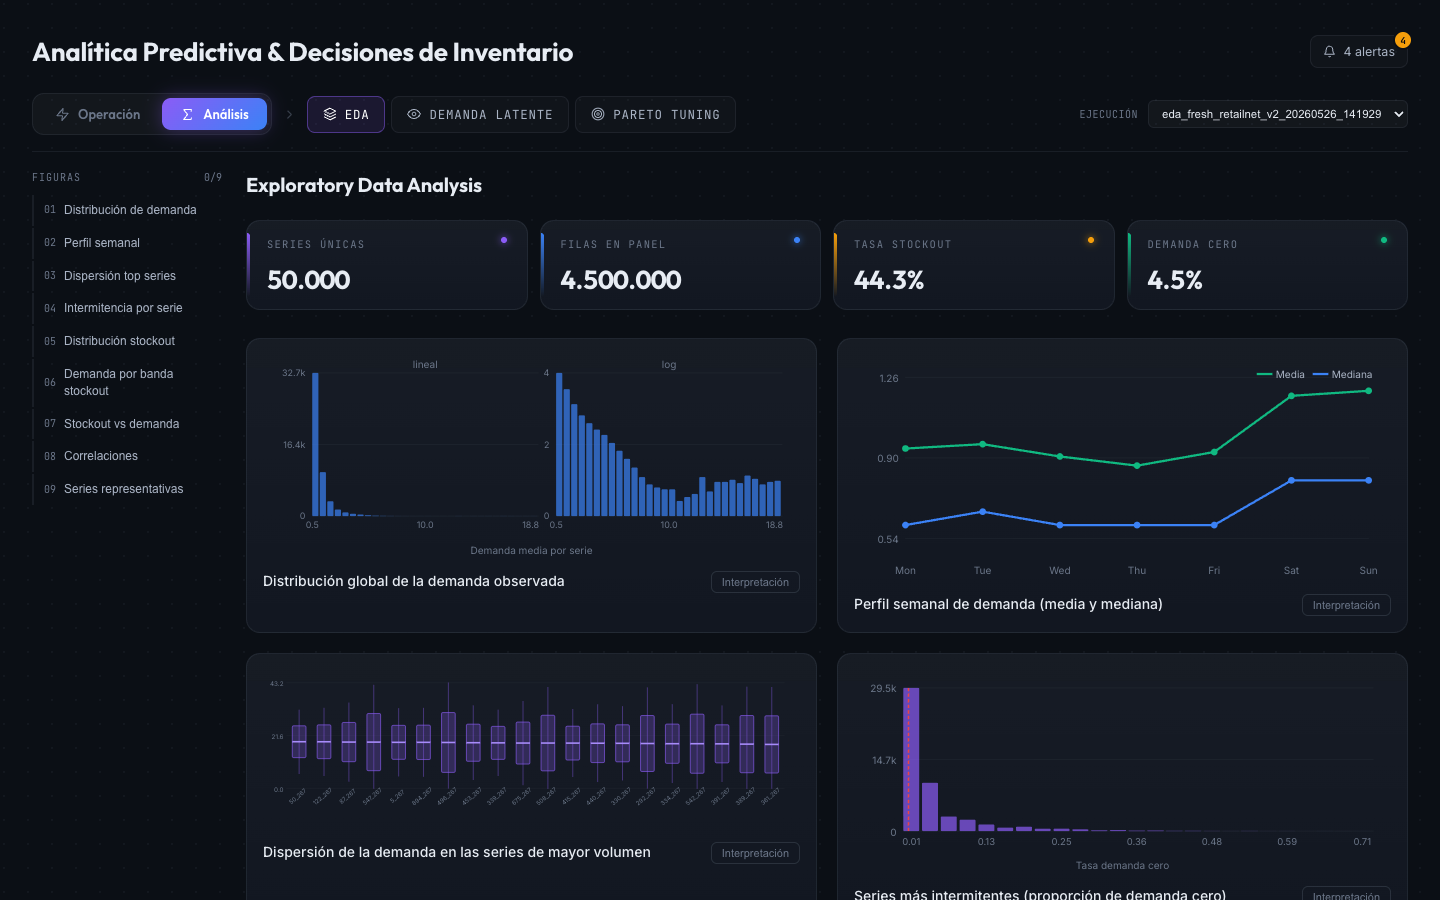
\includegraphics[width=\textwidth,height=0.82\textheight,keepaspectratio]{figures/dashboard/ui_eda_overview.png}
    \caption{Vista \textit{EDA} del plano de Análisis. Panel resumen con estadísticos globales del dataset (50.000 series únicas, 4,5\,M filas, tasa de stockout 44,3\,\%) y las nueve figuras exploratorias, redibujadas como SVG en servidor a partir de los CSV que produce el módulo de análisis exploratorio. Cada figura conserva su interpretación escrita y un enlace al PNG original a resolución completa.}
    \label{fig:ui_eda_overview}
\end{figure}


\begin{figure}[H]
    \centering
    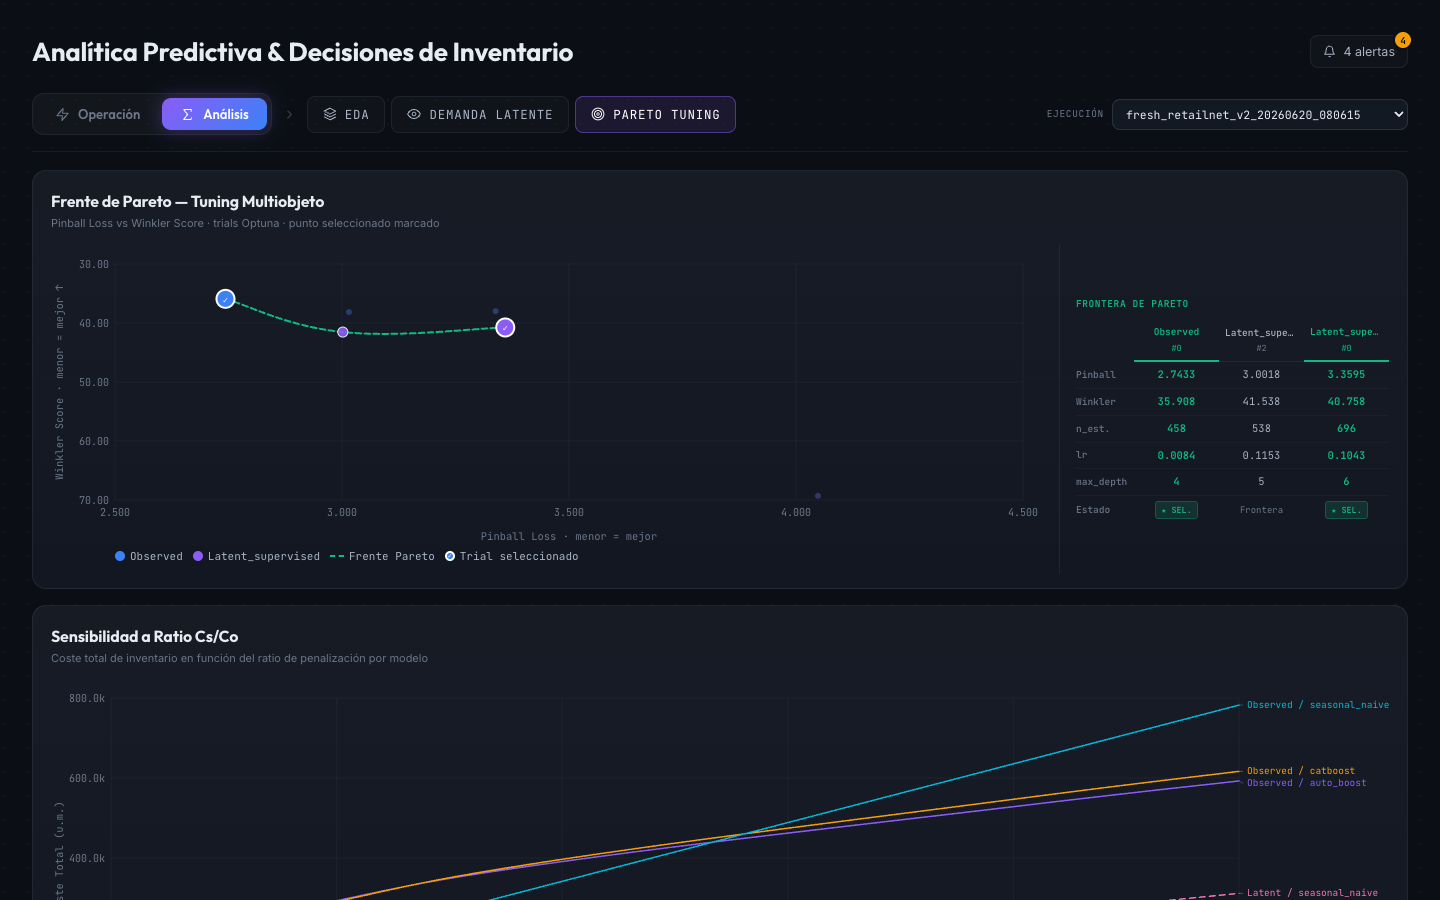
\includegraphics[width=\textwidth,height=0.82\textheight,keepaspectratio]{figures/dashboard/ui_pareto_tuning.png}
    \caption{Vista \textit{Pareto Tuning} del plano de Análisis, con los tres bloques que la componen. Arriba, el frente de la búsqueda multiobjetivo que nombra la propia tarjeta (\texttt{forecasting\_catboost\_v4}, 60 \textit{trials}): cada punto es una configuración situada por su \textit{pinball loss} y su \textit{Winkler score}, en verde las no dominadas y en violeta las dominadas, y a su derecha los hiperparámetros de la que minimiza el \textit{pinball} sobre el frente. En el centro, la sensibilidad al ratio $c_u/c_o$, con cada serie normalizada a su propio rango para que quepan en un eje común. Abajo, el \textit{backtest} de coste justo, que es la comparación que sí ordena las estrategias de reconstrucción (Sección~\ref{sec:resultados_gemelo}).}
    \label{fig:ui_pareto_tuning}
\end{figure}

% !TEX root = ../main.tex
\chapter[Búsqueda de hiperparámetros del imputador]{Búsqueda de Hiperparámetros del Imputador Supervisado}
\label{anx:tuning_imputador}

La estrategia de imputación supervisada descrita en la Sección~\ref{sec:demanda_censurada} se
apoya en un regresor LightGBM auxiliar. Este anexo documenta la búsqueda de hiperparámetros de
ese modelo, que constituye un procedimiento independiente del ajuste del modelo de
\textit{forecasting} y que se ejecuta como un modo de ejecución propio del sistema
(\texttt{run\_mode = tune\_imputation}). Se recoge aquí, y no en el cuerpo de la memoria, porque
su resultado no modifica la configuración del sistema final: lo que aporta es una lección
metodológica sobre la validez de una búsqueda de hiperparámetros, y el material que la sostiene.

\section{Protocolo}

La dificultad de fondo es que la demanda latente de un día con rotura real es un contrafactual
no observable, de modo que no existe verdad-terreno contra la que medir. La búsqueda opera por
tanto sobre el mismo protocolo de censura sintética de la
Sección~\ref{sec:imputacion_censura_sintetica}: se censura artificialmente una fracción de los
días limpios, se reconstruyen y se compara la estimación con la demanda conocida.

El espacio de búsqueda comprende \textbf{trece hiperparámetros}, con cotas acotadas en la
Tabla~\ref{tab:tuning_espacio}, recorridos por 300 \textit{trials} del muestreador gaussiano de
Optuna. Dos decisiones de diseño gobiernan el procedimiento:

\begin{itemize}
    \item \textbf{Promediado sobre múltiples extracciones.} En una sola extracción de censura
    sintética, la dispersión del error entre \textit{trials} (entre el 12\% y el 40\% según la
    medición) es un orden de magnitud mayor que las diferencias reales entre conjuntos de
    hiperparámetros (en torno al 1\%). Una búsqueda de extracción única selecciona por tanto el
    \textit{trial} afortunado, y su propio valor objetivo no es evidencia de mejora alguna: una
    ejecución que reportó un $-1{,}4\%$ en la muestra de selección midió $-0{,}32\%$, con
    intervalo de confianza cruzando el cero, sobre extracciones nuevas. El objetivo promedia
    en consecuencia sobre 15 extracciones.
    \item \textbf{Series disjuntas entre selección y validación.} Las semillas de censura
    disjuntas no bastan: cada extracción censura el 30\% del mismo conjunto de días limpios, de
    modo que tras $n$ extracciones el solapamiento es de $1 - 0{,}7^n$ y los dos conjuntos
    convergen sobre las mismas filas (se midió un 82{,}4\% de solapamiento con 5 y 10
    extracciones). La separación se hace por tanto sobre series: 35 series para seleccionar y
    15 reservadas para validar, con 25 extracciones sobre estas últimas.
\end{itemize}

El ganador solo se persiste si el intervalo de confianza al 95\% de la mejora media sobre las
extracciones de validación queda \textbf{íntegramente por debajo de cero}, y además solo si bate
tanto a los hiperparámetros por defecto como al campeón que ya estuviera en disco.

\begin{table}[htbp]
    \centering
    \small
    \begin{tabular}{llll}
        \toprule
        \textbf{Hiperparámetro} & \textbf{Cotas} & \textbf{Hiperparámetro} & \textbf{Cotas} \\
        \midrule
        \texttt{n\_estimators} & 50 -- 3.000 & \texttt{subsample} & 0,4 -- 1,0 \\
        \texttt{max\_depth} & 2 -- 12 & \texttt{learning\_rate} & 0,005 -- 0,3 (log) \\
        \texttt{num\_leaves} & 2 -- 1.024 & \texttt{colsample\_bytree} & 0,3 -- 1,0 \\
        \texttt{min\_child\_samples} & 2 -- 100 & \texttt{reg\_alpha} & $10^{-8}$ -- 100 (log) \\
        \texttt{min\_data\_per\_group} & 1 -- 100 & \texttt{reg\_lambda} & $10^{-8}$ -- 100 (log) \\
        \texttt{max\_bin} & 8 -- 255 & \texttt{cat\_smooth} & 0 -- 50 \\
        \texttt{subsample\_freq} & 0 -- 1 & & \\
        \bottomrule
    \end{tabular}
    \caption{Espacio de búsqueda de la sintonización del imputador supervisado. La cota superior
    de \texttt{n\_estimators} responde a una restricción de cómputo y está justificada por
    medición: a 500 series un ajuste de 8.000 árboles cuesta unos 34 segundos, lo que situaría
    una búsqueda de 300 \textit{trials} en torno a las 43 horas. Lo que se sacrifica al recortar
    a 3.000 son 0{,}0037 de MAE, cifra inferior a los 0{,}0059 de anchura del intervalo de
    validación que decide la persistencia, de modo que el recorte no puede alterar el veredicto.}
    \label{tab:tuning_espacio}
\end{table}

\section{Resultado: la ganancia se invierte con la escala}

Sobre el protocolo descrito, la búsqueda encuentra una configuración que mejora el error de
reconstrucción un \textbf{5{,}33\%} frente a los hiperparámetros por defecto, con un intervalo
de confianza al 95\% de $[-0{,}0199,\ -0{,}0120]$, enteramente por debajo de cero.

Ese resultado, sin embargo, no es transferible. Al repetir la medición variando únicamente el
número de días limpios con los que se ajusta el imputador, y manteniendo todo lo demás
constante, la ganancia se reduce de forma monótona y termina cambiando de signo
(Tabla~\ref{tab:tuning_reversion}).

\begin{table}[htbp]
    \centering
    \small
    \begin{tabular}{rlr}
        \toprule
        \textbf{Filas limpias de ajuste} & \textbf{Periodo de evaluación} & \textbf{Ganancia} \\
        \midrule
        467 (15 series reservadas) & series disjuntas & $-5{,}33\%$ \\
        595 (últimos 30 días de 50 series) & tiempo disjunto & $-4{,}34\%$ \\
        1.930 (50 series completas) & tiempo disjunto & $-1{,}72\%$ \\
        14.243 (500 series) & tiempo disjunto & $\mathbf{+12{,}44\%}$ \\
        18.310 (500 series más holdout) & semana de holdout & $\mathbf{+13{,}20\%}$ \\
        \bottomrule
    \end{tabular}
    \caption{Efecto del tamaño del conjunto de ajuste del imputador sobre la ganancia de la
    sintonización. Signo negativo indica mejora. Las dos últimas filas coinciden sobre periodos
    de evaluación distintos, lo que descarta el calendario como explicación y señala a la escala.}
    \label{tab:tuning_reversion}
\end{table}

La lectura es que \textbf{el tamaño del conjunto con el que se ajusta el imputador no es un
detalle del montaje experimental, sino la variable que decide la respuesta}. Los mismos
hiperparámetros que mejoran un 5\% con 467 filas de ajuste resultan un 12\% \emph{peores} que no
sintonizar a la escala de 500 series, que es precisamente la escala a la que el sistema ejecuta
la comparación de estrategias del Capítulo~\ref{chap:resultados}. La causa es reconocible: un
conjunto de ajuste pequeño premia configuraciones fuertemente regularizadas que dejan de ser
ventajosas cuando hay datos suficientes.

De ahí se derivan dos consecuencias prácticas. La primera es que un fichero de hiperparámetros
sintonizados solo es válido en el entorno del tamaño de ajuste con el que se obtuvo, y esa
condición no puede expresarse en el propio fichero, por lo que se registra explícitamente en los
metadatos de la búsqueda. La segunda, y es la que justifica la decisión del sistema final, es
que \textbf{las cifras de reconstrucción del Capítulo~\ref{chap:resultados} se obtienen con los
hiperparámetros por defecto}, no con los sintonizados: a la escala a la que se publican, los
defectos son la mejor opción disponible.

\section{Validación del buscador}

Un resultado como el anterior invita a una objeción legítima: que la reversión sea un artefacto
del muestreador empleado y no una propiedad del problema. Para acotarla se repitió la búsqueda
completa con los dos muestreadores disponibles, el basado en procesos gaussianos y el
\textit{Tree-structured Parzen Estimator}, sobre tres semillas comunes y 300 \textit{trials}
cada uno, en un total de unas 14 horas de cómputo (Tabla~\ref{tab:tuning_samplers}).

\begin{table}[htbp]
    \centering
    \small
    \begin{tabular}{rrrrrr}
        \toprule
        \textbf{Semilla} & \textbf{GP} & \textbf{TPE} & \textbf{Diferencia} & \textbf{GP (min)} & \textbf{TPE (min)} \\
        \midrule
        7 & $-6{,}32\%$ & $-6{,}69\%$ & $+0{,}37$ pp & 116 & 198 \\
        42 & $-7{,}62\%$ & $-4{,}56\%$ & $-3{,}06$ pp & 86 & 121 \\
        1.234 & $-6{,}29\%$ & $-7{,}48\%$ & $+1{,}19$ pp & 127 & 177 \\
        \midrule
        \textbf{Media} & $\mathbf{-6{,}74\%}$ & $\mathbf{-6{,}24\%}$ & $\mathbf{-0{,}50}$ \textbf{pp} & \textbf{110} & \textbf{165} \\
        \bottomrule
    \end{tabular}
    \caption{Comparación pareada de muestreadores sobre semillas comunes. La diferencia media
    entre ambos (0{,}50 puntos porcentuales) es cuatro veces menor que su desviación entre
    semillas (2{,}26 puntos), y el signo se invierte según la semilla.}
    \label{tab:tuning_samplers}
\end{table}

La conclusión es un \textbf{resultado nulo}: con tres semillas, el ruido entre extracciones
domina por completo la elección de muestreador, de modo que ambos conducen al mismo sitio y la
reversión de la sección anterior no es atribuible a ninguno de los dos. Lo que sí resulta
concluyente, y es la razón por la que el sistema emplea el muestreador gaussiano, es que este
resulta un 34\% más rápido y gana en las tres semillas sin excepción.

Dos observaciones adicionales del mismo experimento. Las seis búsquedas baten a los
hiperparámetros por defecto con el intervalo de confianza íntegramente por debajo de cero, entre
el $-4{,}56\%$ y el $-7{,}62\%$, lo que confirma que a esa escala de ajuste la ganancia es real
con independencia del muestreador. Y las configuraciones ganadoras \emph{no se parecen entre sí}:
\texttt{num\_leaves} recorre de 40 a 219, \texttt{n\_estimators} de 687 a 3.000 y
\texttt{learning\_rate} de 0{,}015 a 0{,}052, produciendo mejoras casi idénticas. La superficie
de respuesta es plana en la región buena, que es la misma observación con la que se justificó
promediar sobre múltiples extracciones.


\backmatter
% --- Bibliografía ---
\bibliographystyle{ieeetr}
\bibliography{references}

\end{document}
